% input files

\section{Банаховы пространства}
\sbs{40}{Нормированные векторные и банаховы пространства}

\begin{to_def}
	Векторное $E$ -- \textbf{нормировано}, если $\forall v \in E$ имеется $\|v\|$ такое, что:
	\begin{itemize}
		\item Однородность: $\|\alpha v\| = |\alpha| \|v\|$
		\item Неравенство треугольника: $\|v + w\| \leq \|v\| + \|w\|$
		\item Невырожденность: $\|v\| = 0 \Leftrightarrow v = 0$
	\end{itemize}
\end{to_def}

Можно эквивалентно определить норму единичным шаром с центром в $B_0(1)$:
\begin{equation*}
	\|x\| = \inf \{|1/t| \mid t x \in B_0(1)\}
	\hspace{1 cm}
	\text{where }
	B_{c}(r) = \{x \in E \mid \|x-c\| \leq r\}.
\end{equation*}

\begin{to_def}
	Полное нормированное пространство называется \textbf{банаховым}.
\end{to_def}

Так например, $L_p$ и $C[a, b]$ (с нормой $\|\cdot\|_{\infty}$) -- банаховы, а $C[a, b]$ в $L_2$ не ялвяется полным. 




\sbs{41}{Теорема Бэра в банаховом пространстве}

\begin{to_thr}
	Счетное ${U_k}$ -- открытых всюду плотных подмножеств банахова $E$ имеет $\bigcap_k U_k \neq \varnothing$.
\end{to_thr}

\begin{to_con}
	Если банахово $E$ покрыто счетным $(Z_k)$ замкнутых множеств, то $\exists m \colon \textnormal{int}\,Z_m \neq \varnothing$.
\end{to_con}

\begin{to_thr}[Неподвижные точки сжимающих отображений]
	Для банахово $E$ замкнутого $X \subset E$ отображение $f \colon X \to X$ -- \textbf{сжимающее}, то есть
	\begin{equation*}
	 	\exists C <1 \colon \forall x,y \in X \, \|f(x) - f(y)\| \leq C\|x-y\|.
	 \end{equation*} 
	 Имеет неподвижную точку $x \in X$ такую, что $f(x) = x$.
\end{to_thr}
\sbs{42}{Двойственное к банахову пространство}

\begin{to_def}
	Для нормированного $E$ введм двойственное $E'$ -- линейных оторажений $\lambda \colon E \to \mathcal{R]}(\mathcal{C})$. Норма:
	\begin{equation*}
		||\lambda|| = \sup \{ |\lambda(x)| \mid ||x|| \leq 1\}
		\hspace{1 cm}
		\Longleftrightarrow
		\hspace{1 cm}
		\forall x \in E \, |\lambda(x)| \leq ||\lambda|| \cdot ||x||.
	\end{equation*}
\end{to_def}

\begin{to_lem}
	Линейный функционал $\lambda \in E'$ непрерывен \textbf{тогда и только тогда}, когда $||\lambda|| \leq +\infty$. 
\end{to_lem}

\begin{to_thr}
	Двойственное $E'$к нормированному $E$ -- полно по своей норме.
\end{to_thr}
\sbs{43}{Теорема Банаха-Штейнгауза}

\begin{to_thr}[Теорема Банаха-Штейнгауза]
Пусть семейство $Y \subset E'$ $ \ \forall x \in E$ $ \ \ \{\lambda(x) \mid  \lambda \in Y\}$ -- ограничено. \textbf{Тогда } $Y$ ограничено в смысле нормы $E'$.    
\end{to_thr}

\sbs{44}{Расходимость рядов Фурье}
\begin{to_thr}
	Существует $2 \pi$-периодическая функция, ряд Фурье которой расходится в точке $0$.
\end{to_thr}
% \input{tickets/45_Example_44}
\sbs{46}{Непрерывне линейные отображения}
\begin{to_def}
	\textbf{Норма} линейного $A \colon E \to F$ между банаховыми --- $\|A\| = \sup\{\|A(x)\| \mid x \in E , \|x\| \leq 1\}$.
\end{to_def}
Можно сформулировать утверждения:
\begin{equation*}
	\forall x \in E, \, \|Ax\| \leq \|A\| \cdot \|x\|
\end{equation*}
и для $f \colon E \to F$ и $g \colon F \to G$ верно:
\begin{equation*}
	\|g \circ f\| \leq \|g\| \cdot \|f\|.
\end{equation*}
Ядро отображения между банаховыми это просто $\ker A = \{x \in E \mid A x = 0\} $.
\sbs{47}{Факторпространство банахового пространства}
\begin{to_def}
	Если $G \subset E$ -- замкнутое неполное подпространство $E$, то на факторпрострнастве $E/G$ \textbf{норма}:
	\begin{equation*}
		||x+G|| = \inf \{||x+y|| \mid y \in G\} = \inf \{||x-y|| \mid y \in G\} = \text{dist}(x,G) = \text{dist}(0,x+G).
	\end{equation*}
\end{to_def}
\begin{to_lem}
	Определенная выше $||\cdot|| \colon E/G \to \mathcal{R}$ для замкнутого $G \subset E$ в банаховом $E$ явялется нормой.
\end{to_lem}

\begin{to_lem}
	Естественная проекция $\pi \colon E \to E/G$ для замкнутого $G \in E$ имеет единичную норму.
\end{to_lem}

\begin{to_lem}
	Факторпространство $E/G$ банохова пространства по замкнутому подпространству полно.
\end{to_lem}
\sbs{48}{Изоморфизм непрерывных линейных отображений}

\begin{to_lem}
	Если отображение банаховых $A \colon E \to F$ непрерывно, то соответствующее $\bar{A} \colon E/\ker A \to F$ тоже непрерывно и $\|\bar{A}\| = \|A\|$.
\end{to_lem}

\begin{to_def}
	Линейное отображене банаховых $A \colon E \to F$ --- \textbf{изоморфизм}, если $A$ непрерывно и $\vc{A}$ тоже непрерывно.
\end{to_def}

\begin{to_def}
	Если линейное непрерывное из банаховых $A \colon E \to F$ имеет замкнутый $\Im A(E)$, то оно порождает изоморфизм $E/\ker A \to A(E)$.
\end{to_def}
\sbs{Эпсилон-сети, предкомпактность и вполне ограниченность}

\begin{to_def}
	Для топологического пространства $M$, его $X\subseteq M$ --- \textbf{предкомпактным}, если $\overline{X}$ -- компактно.
	\label{def_9.69}
\end{to_def}

\begin{to_def}
	$X\subseteq M$ называется \textbf{вполне ограниченным}, если $\forall \varepsilon > 0 \, \exists N \subseteq X$ -- конечная $\varepsilon$-сеть. (равносильно и утверждение с $N\subset X$)
	Или $\forall \varepsilon >0$, $X$ покрывается конченым набором шаров с центрами в $X$ и радиусами $\varepsilon$.
	\label{def_9.70}
\end{to_def}

\begin{to_thr}
	Для полного метрического пространства $M$, его $X \subseteq M$ -- компактно $\Longleftrightarrow$ $X$ -- вполне ограничено.
	\label{thr_9.73}
\end{to_thr}
\sbs{Теорема Арцела-Асколи}
\begin{to_def}
	Множество функций $X \subset C(K)$(над метрическим компактом) \textbf{равностепенно непрерывно} , если 
	\begin{equation*}
		\forall \varepsilon >0 \, \exists \delta > 0 \colon \forall f \in X\, \forall x, y \in K, \, \rho(x,y) < \delta \Leftrightarrow |f(x) - f(y)| < \varepsilon.
	\end{equation*}
	Если все функции ещё и $L$-липшецивы, то $|f(x) - f(y)| = L \rho(x,y)$.
\end{to_def}

\begin{to_def}
	\textbf{Модуль непрерывности} липшецивых функций:
	\begin{equation*}
		\omega_X(\delta) = \sup \left\{|f(x) - f(y)| \mid f \in X, \, \rho(x,y) < \delta \right\}.
	\end{equation*}
	И тогда,
	$X$ -- равностепенно непрерывно $\Longleftrightarrow$ $\omega_X(\delta) \to 0$ при $\delta \to +0$.
\end{to_def}


\begin{to_thr}[Арцела-Асколи]
	Множество $X \subset C(K)$ предкомпактно $\Longleftrightarrow$ $X$ равномерно ограниченно и равностепенно непрерывно.
\end{to_thr}

\section{Гильбертовы пространства}
\sbs{51}{Гильбертово пространство}
\begin{to_def}
	Если норма в банаховом $E$ порождается $+$определённым $\|x\| = \sqrt{(x,x)}$, то $E$ --- \textbf{гильбертово}. 
\end{to_def}

\begin{to_thr}[Неравнество Коши-Буняковского]
	$|(x,y)| \leq \|x\| \cdot \|y\|$
	\begin{equation*}
		(ax + by, ax + by) \geq 0 
		\hspace{0.5 cm}
		\Leftrightarrow
		\hspace{0.5 cm}
		|a|^2 \|x\|^2 + a \bar{b} (x,y) + b \bar{a} \overline{(x,y)} + |b|^2 \|y\|^2 \geq 0
	\end{equation*}
\end{to_thr}

\begin{to_thr}
	Вещественное банахаво $E$ -- гильбертово \textbf{тогда и только тогда}, когда $\forall x,y \in E$:
	\begin{equation*}
		\|x+y\|^2 + \|x-y\|^2 = 2 \|x\|^2 + 2 \|y\|^2.
	\end{equation*}
\end{to_thr}
\sbs{52}{Полнота и замкнутость ортонормированной системы в гильбертовом пр-ве}
\begin{to_def}
	Последовательность векторов $(\varphi_k)$ --- \textbf{полная система векторов}  в банаховом $E$, если $\overline{\langle \varphi_k\rangle} = E$. Другими словами $\forall x \in E$ и $\forall >0$ найдется конечная $a_1 \varphi_1 + \ldots + a_n \varphi_n$ такая, что $\|x - a_1 \varphi_1 - \cdots - a_n \varphi_n\|<\varepsilon$.
\end{to_def}

\begin{to_def}
	$(\varphi_k)$ --- \textbf{замкнутая система векторов} в гильбертовом $H$, если в $\forall x \in H \colon (x, \varphi_k) = 0, \, \forall k$.
\end{to_def}

\begin{to_thr}
	$\forall \varphi_k$ -- ортогональной в гильбертовом $H$ эквивалентны утверждения:
	\begin{itemize}
		\item полнота системы;
		\item замкнутость системы;
		\item сходимость ряда Фурье $\forall x \in H$ по системе $(\varphi_k)$ к $x$;
		\item равенство Парсеваля для коэффициентов Фурье $\forall x \in H$ по данной системе.
	\end{itemize}
\end{to_thr}


\sbs{53}{Изометрии гильбертовых пространств}
\begin{to_def}
	Линейное $A\colon E \to F$ --- \textbf{изометрия}, если оно биективно и сохраняет норму: $||A|| = ||A^{-1}|| = 1$.
\end{to_def}

\begin{to_lem}
	Изометрия гильбертовых пространств сохраняет скалярное произведение.
\end{to_lem}

\begin{to_thr}[Рисса-Фишера]
	$\forall H$, в котором $\exists$ счетная полная система элементов, изометрична $\mathbb{C}^n (\mathbb{R}^n)$ или комплексному(действительному) варианту бесконечномерного пространства последовательностей $l_2 = L_2(\mathcal{N})$.
\end{to_thr}
\sbs{54}{Метрическая проекция и двойственное к гильбертову пр-во}

\begin{to_thr}
	$V\subset H$ -- замкнутое линейное подпространство (афинное) гильбертова. $\forall x \in H \, \exists ! P_V(x) \in V$ ближайший к $x$ то есть $\|x - P_V(x)\| = \text{dist} (x,V)$.
\end{to_thr}

\begin{to_thr}
	Если $V\subset H$ -- замкнутое линейное подпространство, то \textbf{метрическая проекция} $P_V \colon H \to V$ линейна, $\|P_V\| = 1$ при $V \neq 0$ и имеет место ортогональное разложение в прямую сумму замкнутых подпространств $H = V \oplus \ker P_V$.
\end{to_thr}
\sbs{55}{Двойственное к гильбертову пространству}
\begin{to_thr}
	$\forall y \in H \colon \lambda_y(x) = (x,y)$. Тогда $\lambda_y \in H', \, \|\lambda_y\| = \|y\|$ и все элементы двойственного пространства $H'$ имеют такой вид.
\end{to_thr}

\section{Обобщенные функции}
\sbs{63}{Пространство $\mathcal{E}$ и топология в нём}
Будем рассматривать функции на действительной прямой, чтобы не отвелкаться на технические тонкости. И так
\begin{to_def}
	$\mathcal{E}(\mathcal{R}) = C^{\infty}(\mathcal{R})$. Топологию в таком пространстве зададим полунормами:
	\begin{equation*}
		||f||_{K,k} = \sup \{ |f^{(k)}| \mid x \in K\},
	\end{equation*}
	где $K \subset \mathcal{R}$ -- компакты и $k \in \mathcal{Z}_+$. Ну то есть имеем семейство открытых:
	\begin{equation*}
		U_{K,k,\varepsilon} (f_0) = \{f \mid ||f - f_0||_{K,k} < \varepsilon\}.
	\end{equation*}
\end{to_def}

\begin{to_thr}
	Пространство $\mathcal{E}$ -- полно.
\end{to_thr}
\sbs{64}{Связь непрерывности и ограниченности}
\begin{to_thr}
	$\forall$ непрерывного линейного $\lambda \in \mathcal{E}'(\mathbb{R})$ $\exists C>0, \, k \in \mathcal{Z}_+,\, K= [-m,m]:$
	\begin{equation*}
		|\lambda(\varphi)| \leq C \text{max} \{||\varphi||_{K,l} \mid 0\leq l \leq k\} = C \sup \{|\varphi^{(l)}(x)| \mid x \in [-m,m], 0 \leq l \leq k\}.
	\end{equation*}
\end{to_thr}
\sbs{65}{Описание через интегрирование производных по отрезку}
\begin{to_thr}
	$\forall \lambda \in \mathcal{E}'(\mathbb{R})$ задаётся интегрированием проихводных $\varphi\in \mathcal{E}(\mathbb{R})$ по борелевским мерам со знаком конечной вариации на некотором отрезке:
	\begin{equation*}
		\lambda(\varphi) = \int_{-m}^{m} \varphi d \mu_0 + \int_{-m}^{m} \varphi' d \mu_1 + \cdots + \int_{-m}^{m}\varphi^{(k)} d \mu_k.
	\end{equation*}
\end{to_thr}
\sbs{66}{Прстранство $\mathcal{D}$ и сходимость в нём}
В основном, когда речь заходит про обобщенные функции имеется в виду именно пространство $D'$
\begin{to_def}
	$(\varphi_k) \subset \mathcal{D}(\mathcal{R})$ сходится к $\varphi_0 \in \mathcal{D}(\mathcal{R})$, если $\text{supp} \varphi_k \in [-m, m]$ и $\forall l \in \mathcal{Z}^+$ равномерно $\varphi_k^(l) \overset{[-m, m]}{\rr} \varphi_0^{(l)}$.
\end{to_def}

С помощью сходимости в $\mathcal{D}$ определим непрерывные линейные функционалы из которых получим $\mathcal{D}'(\mathcal{R})$. И если не оговорено обратного, именно его мы будем называть \textbf{пространством обобщенных функций} 
\sbs{67}{Пространство обобщённых функций. Регулярные и нерегулярные}
\begin{to_def}
	$\forall$ локально $\text{L}_1 \ni f \colon \mathcal{R} \to \mathcal{R}$ задаёт $\lambda_f \in \mathcal{D}'(\mathcal{R})$ \textbf{регулярные функции}:
	\begin{equation*}
		\lambda_f(\varphi) = \int_{-\infty}^{\infty} f(x) \varphi(x) d x
	\end{equation*}
\end{to_def}

\begin{to_lem}
	Локально интегрируемые $f$ и $g$ задаются $\lambda_f = \lambda_g \in \mathcal{D}'(\mathcal{R})$ \textbf{тогда и только тогда}, когда они отличаются на множестве меры нуль. 
\end{to_lem}

Помимо регулярных в пространстве $\mathcal{D}'$ лежат ещё нерегулярные. Давайте посмотрим на самую популярную из них.

\begin{to_def}
	\textbf{Дельта-функция} или функция Дирака
	\begin{equation*}
		\lambda_\delta (\varphi)= \int_{-\infty}^{\infty} \delta(x) \varphi(x) d x = \varphi(0),
		\hspace{0.5 cm}
		\int_{-\infty}^{\infty} \delta(x) d x = 1
		\hspace{0.5 cm}
		\delta(x) = \left\{
		\begin{aligned}
			&0, \, &x \neq 0\\
			&\infty, \, &x = 0
		\end{aligned}\right.
	\end{equation*}
	Также можно говорить о смещенной дельтта-функции:
	\begin{equation*}
		\lambda_\delta (\varphi) = \int_{-\infty}^{\infty} \delta(x-a) \varphi(x) d x = \varphi(a)
	\end{equation*}
\end{to_def}
\sbs{68}{Топология и сходимость в D'}
\begin{to_def}
	В $\mathcal{D}'(\mathcal{R})$ используется $\star$-слабая топология соответствующая поточечной сходимости. Предбаза топологии:
	\begin{equation*}
		U_{\varphi,a,b} = \{\lambda \in \mathcal{D}'(\mathcal{R}) \mid a < \lambda(\varphi) < \beta\},
	\end{equation*}
	для $\varphi \in \mathcal{D}(\mathcal{R})$, $a< b \in \mathcal{R}$. Сходимость в $\mathcal{D}'(\mathcal{R}): \lambda_n \to \lambda_0$ будем понимать в смысле $\forall \varphi \in \mathcal{D}(\mathcal{R}): \lambda_n(\varphi) \to \lambda_0(\varphi)$.
\end{to_def}

\begin{to_thr}
	Пусть $(f_k)$ локально интегрируемых: $\int_{-\infty}^{+\infty} f_n(x) d x = 1$. Пусть $\exists C >0 \colon |\int_{a}^{b} f_n(x) d x|<C$ при этом $C$ не зависит $a,b,n$. Пусть ещё $\forall \delta>0$ (внимание, это не дельта-функция):
	\begin{equation*}
		\lim_{n \to \infty} \int_{\delta}^{+\infty} f_n(x) d x = \lim_{n \to \infty} \int_{-\infty}^{\delta} = 0.
	\end{equation*}
	\textbf{Тогда} $\lambda_{f_n} \to \delta_0$ в смысле $\mathcal{D}'(\mathcal{R})$
\end{to_thr}

\begin{to_suj}
	Получаем свойство интергала Дирихле: $\frac{\sin \lambda x}{\pi x} \to \delta_0$ при $\lambda \to \infty$ в смысле сходимости в $\mathcal{D}'(\mathcal{R})$.
\end{to_suj}
\sbs{69}{Дифференцирование обобщенных функций}
Общая идея выведения действия какой-либо операции на обобщенные функции -- проделать её с регулярной, а затем обобщить и на нерегулярные. Будем теперь писать действия обобщенной функции как: $\lambda_f(\varphi) = \langle \lambda_f, \varphi\rangle$.

\begin{to_def}
	Производная от обобщенной функции: $\langle \lambda', \varphi \rangle  = - \langle \lambda, \varphi'\rangle$.
\end{to_def}
Здесь это вынесено определением, но несложно показать интегрируя по частям функцию с компактным носителем:
\begin{equation*}
	\langle \lambda_f', \varphi \rangle = - \int_{-\infty}^{+\infty} f'(x)\varphi(x) d x = - \int_{-\infty}^{+\infty} f(x) \varphi'(x)d x
\end{equation*}
Таким образом получили линейный непрерывный функционал.

Можно сформулировать утверждения вытекающие из определения производной:
\begin{enumerate}
	\item $\forall f \in \mathcal{D}'$ имеет производные всех порядков;
	\item Если $(f_k)\to f$ для обобщенных. То и $f_k' \to f'$. И так далее;
\end{enumerate}
 
 \begin{to_lem}
 	Всякий сходящийся ряд из обобщенных функций можно дифференцировать почленно любое количество раз.
 \end{to_lem}

 И для примера рассмотрим тоже популярную функцию
 \begin{equation*}
 	f(x) = \left\{
 	\begin{aligned}
 		&1, \, x > 0\\
 		&0, \, x \leq 0
 	\end{aligned}\right.
 	\hspace{0.5 cm}
 	\leadsto
 	\hspace{0.5 cm}
 	\langle \lambda_f,\varphi\rangle = \int_{0}^{\infty} \varphi(x) d x
 \end{equation*}
 Это \textbf{Функция Хевисайда} она обладает хайповым свойством -- её производная это дельта-функция:
 \begin{equation*}
 	\langle \lambda_f', \varphi\rangle = - \langle \lambda_f, \varphi'\rangle = - \int_{0}^{\infty} \varphi'(x) d x = \varphi(0).
 \end{equation*}

Покажем ещё непрерывность в смысле топологии по конспекту Романа Николаевича:
\begin{equation*}
	\lambda' \in U_{\varphi,a,b} 
	\hspace{0.3 cm}
	\Leftrightarrow
	\hspace{0.3 cm}
	a <\lambda'(\varphi) < b 
	\hspace{0.3 cm}
	\Leftrightarrow
	\hspace{0.3 cm}
	a < - \lambda(\varphi') < b
	\hspace{0.3 cm}
	\Leftrightarrow
	\hspace{0.3 cm}
	\lambda \in U_{- \varphi', a, b}.
\end{equation*}

\sbs{70}{Умножение на бесконечно гладкую функцию}
\begin{to_def}
	Умножение $\lambda \in \mathcal{D}'(\mathbb{R})$ на $f \in \mathcal{E}(\mathbb{R})$ определим как:
	\begin{equation*}
		\langle \lambda f, \varphi\rangle = \langle \lambda, f \varphi\rangle.
	\end{equation*}
\end{to_def}
При чём у нас есть правило Лейбница \begin{equation*}
		(\lambda f)' = \lambda' f + \lambda f'
\end{equation*}

\begin{to_lem}
	Определение умножения $\lambda f$ корректно, то есть $\lambda f \in \mathcal{D}'(\mathbb{R})$.
\end{to_lem}

\begin{to_lem}
	Произведение $\lambda f$ непрерывно зависит от $\lambda \in \mathcal{D}'(\mathbb{R})$.
\end{to_lem}
\sbs{71}{Носитель распределения из пространства обобщённых функций}
Будем говорить, что для открытого $U \subset \mathbb{R}$ обобщенная функция $\lambda\big|_U = 0$, если $\forall \varphi \in \mathcal{D}(\mathbb{R})\colon \lambda(\varphi) = 0$

\begin{to_lem}
	Пусть для $\lambda \in \mathcal{D}'(\mathbb{R})$ $\exists$ открытые $\{U_\alpha\} \colon \forall \alpha \, \lambda\big|_{U_\alpha} = 0$. \textbf{Тогда} для $U = \bigcup_\alpha U_\alpha$ окажется $\lambda\big|_U = 0$.
\end{to_lem}

\begin{to_def}
	Для $\lambda \in \mathcal{D}'(\mathbb{R})$ положим $Z_\lambda = \bigcup \{U \mid \lambda\big|_U = 0\}$. Введём \textbf{носитель}  $\lambda$ как $\text{supp} \lambda = \mathbb{R} \backslash Z_\lambda$.
\end{to_def}

И ещё пара интересных свойств:
\begin{to_lem}
	$\forall \lambda \in \mathcal{D}'(\mathbb{R})$ с компактным носителем можно однозначно сопоставить элемент $\mathcal{E}'(\mathbb{R})$ с помощью умножения $\lambda$ на функцию с компактным носителем равную единице в окрестности $\text{supp}\lambda$.
\end{to_lem}

\begin{to_thr}
	$\forall \lambda \in \mathcal{D}'(\mathbb{R})$ с компактным носителем является производной некоторого порядка от некоторой регулярной обобщённой функции.
\end{to_thr}
\sbs{72}{Преобразование Фурье для обобщённый функций}
Тут нам уже потрубется пространство $\mathcal{S}(\mathbb{R})$. Так как
\begin{to_def}
	Преобразование Фурье непрерывно переводит $\mathcal{S}(\mathbb{R})$ в $\mathcal{S}(\mathbb{R})$.
\end{to_def}

\begin{to_def}
	$\mathcal{S}(\mathbb{R})$ -- \textbf{пространство бесконечно дифференцируемых функций} $f \colon \mathbb{R} \to \mathbb{C}$, у которрой конечны все полунормы $(k,n \geq 0)$
	\begin{equation*}
		\|f\|_{n,k} = \sup \{x^n f^{(k)}(x) \mid x \in \mathbb{R}\}.
	\end{equation*}
\end{to_def}

Соответсвенно можем определить преобразование Фурье:
\begin{equation*}
	\langle F[\lambda], \varphi\rangle = \langle \lambda, F[\varphi]\rangle.
\end{equation*}

Наверное тут хочется посмотреть на хороший пример: обозначим $F[\delta] = \hat{\delta}$, тогда
\begin{equation*}
	(\hat{\delta}, \varphi) = (\delta, \hat{\varphi}) = \hat{\varphi}(0) = \frac{1}{\sqrt{2 \pi}} \int_{-\infty}^{+\infty} \varphi(x) e^{- i x y} d x\big|_{y=0} = \frac{1}{\sqrt{2 \pi}} \int_{-\infty}^{+\infty} \varphi(x) d x = \left(\frac{1}{\sqrt{2 \pi}}, \varphi\right)
\end{equation*}
Ого, мы полчуили, что $F[\delta] = 1/\sqrt{2\pi}$, а для обратного тогда $F^{-1}[1] = \sqrt{2\pi}\delta$. И подобным же образом получается и прямое преобразование фурье для единицы, что ранее не в обобщенных нам было не доступно.



% % document's head

\begin{center}
    \LARGE \textsc{Домашнее задание №2 курса <<Гармонический анализ>>}
\end{center}

\hrule

\phantom{42}

\begin{flushright}
    \begin{tabular}{rr}
    % written by:
        \textbf{Автор}: 
        & Хоружий Кирилл \\
        &\\
    % date:
        \textbf{От}: &
        \textit{\today}\\
    \end{tabular}
\end{flushright}

\thispagestyle{empty}
\tableofcontents
\newpage


% % \section{Приближение функций}
% \subsection{Протокол BB84}
Пусть есть вертикальная и диагональная поляризация, а также 4 квантовых состояния


шифр Вернама
Протокол Диффи — Хеллмана
Алгоритм RSA

Классическая кирптография: 
    + изученность, стандартизированность
    - не выдерживает создание квантового компьютера

Квантовая криптография:
    + не ставит перехватчик перед вычислительными задачами
    - мало изучены, возможны атаки

Постквантовая криптография:
    + выдерживает существование квантового компьютера
    - недостаточная изученность, авось и классический может взломать


\subsection{Теория Информации}    
пусть $h(p)$ -- информационное содержание события вероятности $p$.
Верно следующее утверждение:
\begin{equation*}
    h(p_1) > h(p_2) \ \ \Leftarrow \ \ p_1 < p_2.
\end{equation*}
Также вполне логично предположить, что $h(1) = 0$, а также что $h(p_1 p_2) = h(p_1)+h(p_2)$. 

Это приводит к функции вида
\begin{equation*}
    h(x) = - \log x = \log_2 \frac{1}{x}
\end{equation*}

\textit{Распределением вероятностей} будем считать некоторый набор $\{p_i\}$ такой, что $\sum p_i = 1$.
Информация, выдаваемая источником может быть найдена, как \textit{матожидание} 
\begin{equation*}
    H(P) = - \sum_i p_i \log p_i,
\end{equation*}
иначе функция называется энтропией Шеннона, -- мера того, насколько неизвестно что выдаст источник. 

Также энтропия Шеннона -- среднее количество вопросов, которые необходимо задать. Ещё это среднее количество битов, которое необходимо, чтобы закодировать выход источника. 

Неравенство Крафта позволяет сформулировать условие к префиксному коду. 

Также можно сформулировать, что разность между практической и теоретической длиной слова $\geq 0$, что соответсвует неравенству Гиббса. 


\begin{itemize}
    \item Коды Хаффмана
    \item Maassen-Uffink entropic
\end{itemize}

\subsection{Измерения в базисе}

Возвращаемся к состояниям 
\begin{align*}
    \cqs{0}{+} &= \qs{0} = \begin{pmatrix}
        1 \\ 0
    \end{pmatrix} \\
    \cqs{1}{+} &= \qs{1} = \begin{pmatrix}
        0 \\ 1
    \end{pmatrix} \\
    \cqs{0}{\times} &= \frac{\qs{0}+\qs{1}}{\sqrt{2}} = \frac{1}{\sqrt{2}} \begin{pmatrix}
        1  \\ 1
    \end{pmatrix} \\
    \cqs{1}{\times} &= \frac{\qs{0}-\qs{1}}{\sqrt{2}} = \frac{1}{\sqrt{2}} \begin{pmatrix}
        1 \\ -1
    \end{pmatrix} \\
\end{align*}
Пусть есть некоторый ортонормированный базис $\{\qs{e_i}\}$ и  состояние $\qs{\xi}$. Вероятность исхода $i$ при измерении $\qs{\xi}$ в базисе $\{\qs{e_i}\}$ равна
\begin{equation*}
    \textnormal{Pr}\, (i) = | \langle e_i | \xi \rangle|^2.
\end{equation*}



\sbsnum{3}{Пространство интегрируемых функций}
\subsubsection*{Неравенства Гёльдера и Минковского}


\begin{to_def}
    \textit{Абсолютно интегрирумыми функциями} на измеримом $X \subseteq \mathbb{R}^n$ называют $f \colon X \mapsto \mathbb{R}$ с конечным интегралом $\int_X |f(x)| \d x$. \textit{Расстоянием}\footnote{
        В силу неравенства $|f(x) - g(x)| \leq |f(x)| + |g(x)|$ расстояние конечно.
    } между функциями $f$ и $g$ будем считать $\int_X |f(x)-g(x)| \d x$.
\end{to_def}

\begin{to_def}
    Обозначим через $L_1 (X)$ факторпространство  линейного пространства абсолютно интегрируемых функций по его линейному подпространству почти всюду равных нулю функций. То есть функции на $0$ расстоянии считаем равными. \textit{Нормой} будем считать
    \begin{equation*}
        \|f\|_1 = \int_X |f(x)| \d x.
    \end{equation*}
\end{to_def}

\begin{to_def}
    Для измеримого по Лебегу $X \subset \mathbb{R}^n$ и числа $p \geq 1$ \textit{факторпространство} измеримых по Лебегу функций на $X$ с конечной (полу)нормой
    \begin{equation*}
        \|f\|_p
        = 
        \left(
            \int_X |f|^p \d x
        \right)^{1/p},
    \end{equation*}
    по модулю функций равных нулю почти всюду,
    назовём $L_p (X)$.
\end{to_def}

\texttt{Очень хорошим, симметричным, актуальным для описания квантовой механики оказывается $L_2$ простран-\\ство, на котором естественно вводить скалярное произведение, его порождающее.} 

 \begin{to_def}
     В комплексном случае норма $L_2$ порождена \textit{скалярным произведением}
     \begin{equation*}
         (f, g) = \int_{-\infty}^{+\infty} f(x) \overline{g(x)} \d x
         \hspace{0.5cm} \longrightarrow \hspace{0.5cm}
         \|f\|_2 = \sqrt{(f, f)}.
     \end{equation*}
 \end{to_def}


\begin{to_thr}[Неравенство Гёльдера]
    Возьмём $p, \, q > 1$ такие, что $1/p + 1/q = 1$. Пусть $f \in L_p (X)$ и $g \in L_q(X)$. Тогда
    \begin{equation*}
        \int_X |fg| \d x \leq \|f\|_p \cdot \|g\|_q.
    \end{equation*}
\end{to_thr}

\begin{proof}[$\triangle$]
    Для доказательства достаточно проинтегрировать неравенство вида
    \begin{equation*}
        |fg| \leq \frac{|f|^p}{p} + \frac{|g|^q}{q}.
    \end{equation*}
    \red{Осталось получить само неравенство.}
\end{proof}

\begin{to_con}
    Для измеримых функций и чисел $p, \, q > 0$, таких что $1/p + 1/q = 1$, имеет место формула
    \begin{equation}
        \label{8_1}
        \|f\|_p = \sup \left\{
            \int_X fg \d x \ \bigg| \  \|g\|_q \leq 1
        \right\}.
    \end{equation}
\end{to_con}


\begin{proof}[$\triangle$]
По неравенству Гёльдера норма $f$ не менее супремума правой части \red{(?)}, более того равенство достигается при выборе
\begin{equation*}
    g(x) = \frac{\sign f(x) |f(x)|^{p-1}}{\|f\|_p^{p-1}}.
\end{equation*}
\end{proof}

\begin{to_def}
    Функция $f \colon V \mapsto \mathbb{R}$ на векторном пространство называется выпуклой, если для любых $x, \, y \in V$ и любого $t \in (0, 1)$ имеет место неравенство
    \begin{equation*}
        f ( (1-t) x + ty) \leq (1-t) f(x) + t f(y).
    \end{equation*}
    Функция называется \textit{строго выпуклой}, если неравенство строгое $\forall x \neq y$ и $t \in (0, 1)$. 
\end{to_def}

\begin{to_lem}
    Если в семействе функций $f_\alpha \colon V \mapsto \mathbb{R}$, $\alpha \in A$, все функции выпуклые, то
    \begin{equation*}
        f(x) = \sup \{f_\alpha (x) \mid \alpha \in A\}
    \end{equation*}
    тоже выпуклая\footnote{
        Если разрешить в определении выпуклости значение $+ \infty$.
    }.
\end{to_lem}


\begin{to_thr}[Неравенство Минковского]
    Для функций $f, \, g \in L_p$ при $p \geq 1$
    \begin{equation*}
        \|f + g\|_p \leq \|f\|_p + \|g\|_p.
    \end{equation*}
\end{to_thr}



\subsubsection*{Полнота пространства интегрируемых функций}

Далее в разделе всегда предполагается суммирование по $k$ от $1$ до $\infty$. Глобально можно сказать, что \texttt{в нормированном пространстве вопрос полноты сводится в вопросу сходимости рядов}, у которых сходятся суммы норм. 

\begin{to_def}
    Назовём последовательность $(f_n)$ \textit{фундаментальной}, если
    \begin{equation*}
        \forall \varepsilon > 0 \ 
        \exists N_\varepsilon \colon 
        \forall n, m \geq N_\varepsilon \
        \|f_n - f_m\|_p < \varepsilon.
    \end{equation*}
\end{to_def}

\begin{to_lem}
    Пусть у последовательности функций $(u_k)$ из $L_p (X)$ сумма
    $\sum \|u_k\|_p$
    оказалась конечной. Тогда $S(x) = \sum u_k (x)$ определена для почти всех $x$ и
    $\|S\|_p \leq \sum \|u_k\|_p.$
\end{to_lem}


\begin{to_lem}
    Пусть у последовательности функций $(u_k)$ из $L_p (x)$ сумма
    $\sum \|u_k\|_p$
    оказалась конечной. Тогда $S(x) = \sum u_k (x)$ определена для почти всех $x$ и
    $S = \sum u_k$
    в смысле сходимости в пространстве $L_p (X)$.
\end{to_lem}


\begin{to_thr}[]
    Пространство $L_p (X)$ полно.
\end{to_thr}



Вообще сходимость в $L_p (X)$ может не означать поточечной сходимости ни в одной точке.

\sbsnum{4}{Приближение функций ступенчатыми и бесконечно гладкими}
\section{Интерференция}


\input{parts/S28}
\input{parts/S30}
\input{parts/S31}
\input{parts/S32}





% \section{Ограниченная вариация, абсолютная непрерывность и осцилляция}
% \sbsnum{5}{Функции ограниченной вариации}
\begin{to_def}
    Функция $f$ на промежутке $I$ имеет \textit{ограниченную вариацию}, если для любых $x_0 < x_1 < \ldots M x_N \in I$ (в любом количестве)
    \begin{equation*}
        |f(x_0) - f(x_1)| + 
        |f(x_1) - f(x_2)| + \ldots +
        |f(x_{N-1}) - f(x_N)| \leq M,
    \end{equation*}
    для некоторой константы $M$. Наименьшую константу $M$ в этом неравенстве назовём вариацией функции $f$ равную $\|f\|_B$, что задаёт \textit{полунормой}.
\end{to_def}


\begin{to_lem}
    Функцию ограниченной вариации на отрезке $[a, b]$ можно представить в виде суммы двух функций $f = u + d$, одна из которых возрастает, а другая убывает. При этом $\|f\|_B = \|u\|_B + \|d\|_B$ и если $f$ была непрерывной, то $u$ и $d$ тоже будут непрерывны.
\end{to_lem}


\red{Дополнить смыслом функций с ограниченной вариацией.}

\sbsnum{6}{Абсолютно непрерывные функции и обобщенная формула Ньютона-Лейбница}
Для формулы Ньютона-Лейбница условие липшицевости можно ослабить до следующего:

\begin{to_def}
    Функция $F$ на промежутке $I$ \textit{абсолютно непрерывна} , если $\forall \varepsilon > 0 \ \exists \delta_\varepsilon > 0$, такое что
    $\forall \, x_1 \leq y_1 \leq x_2 \leq y_2 \leq \ldots \leq x_N \leq y_N \in I$ из неравенства
    \begin{equation*}
        |x_1 - y_1| + |x_2 - y_2| + \ldots + |x_N - y_N| \leq \delta
    \end{equation*}
    следует, что
    \begin{equation*}
        |F(x_1)-F(y_1)| + 
        |F(x_2)-F(y_2)| + 
        \ldots +
        |F(x_N)-F(y_N)| \leq \varepsilon.
    \end{equation*}
    \texttt{
    Говоря неформально, сумма модулей приращений функции на системе непересекающихся отрезков должна \\ стремиться к нулю при суммарной длине системы, стремящейся к нулю.
    } 
\end{to_def}

\begin{to_lem}
    
\end{to_lem}


\begin{to_thr}[]
    Для некоторой $f \in L_1 [a, b]$, всякая обобщенная первообразная $F$ 
    \begin{equation*}
        F(x) = \int_a^x f(t) \d t,
    \end{equation*}
     является абсолютно непрерывной и её производная почти всюду существует и совпадает с $f$.
\end{to_thr}


\begin{to_lem}
    Абсолютно непрерывная на отрезке функция $f$ имеет на нём ограниченную вариацию. Также на отрезке существует разложение $f$ в сумму двух монотонных абсолютно непрерывных функций.
\end{to_lem}


\begin{to_thr}[]
    Абсолютно непрерывная функция $F \colon [a, b] \mapsto \mathbb{R}$ почти всюду имеет производную и является обобщенной первообразной своей производной с выполнением формулы Ньютона-Лейбница
    \begin{equation*}
        F(b) - F(a) = \int_a^b F' (t) \d t.
    \end{equation*}
\end{to_thr}

\red{Легко показать через\ldots ух, ну по \textbf{лемме Безиковича}, посмотреть можно
\href{https://youtu.be/kTzJlaSrK7Y?list=PLthfp5exSWErwR6-3PMFN9w_iGJBdlXfZ&t=4030}{здесь}.}

\begin{to_con}[Обобщенное интегрирование по частям]
    Если $f \in L_1 [a, b]$, а $g$ абсолютно непрерывна, то верна формула интегрирования по частям
    \begin{equation*}
        \int_a^b f g \d x = F(x) g(x) \bigg|_a^b
        - \int_a^b F(x) g'(x) \d x,
    \end{equation*}
    где $F(x) = \int_a^x f(t) \d t$.
\end{to_con}


\begin{to_lem}
    Функция $f \colon [a, b] \mapsto \mathbb{R}$ абсолютно непрерывна тогда и только тогда, когда она может быть сколь угодно близко в $B$-норме приближена кусочно-линейными функциями.
\end{to_lem}

\red{А дальше про борелевские меры на отрезках и интеграл Лебега–Стилтьеса.}



\sbsnum{7}{(до 2.9) Осцилляции и равномерные осцилляции}
\begin{to_def}
    Определим \textit{коэффициент Фурье} (с точностью до умножения на константу)
    \begin{equation*}
        c_f (y) = \int_{-\infty}^{+\infty} f(x) e^{-ixy} \d x.
    \end{equation*}
\end{to_def}

\begin{to_thr}[]
    Если $f \in L_1 (\mathbb{R})$, то $|c_f (y)| \leq \|f\|_1$ и $c_f (y)$ непрерывно зависит от $y$.
\end{to_thr}

\begin{to_thr}[Лемма об осцилляции]
    Если $f \in L_1 (\mathbb{R})$, то выражение
    \begin{equation*}
        c_f (y) = \int_{-\infty}^{+\infty} f(x) e^{-ixy} \d x
    \end{equation*}
    стремится к нулю при $y \to \infty$.
\end{to_thr}

\begin{to_lem}
    Еси производная $f^{(k-1)}$ абсолютно непрерывна и производные до $k$-й включительно\footnote{
        Для $k$-й достаточно существования почти всюду.
    }  находятся в $L_1 (\mathbb{R})$, то
    \begin{equation*}
        c_f (y) = o \left(\frac{1}{y^k}\right),
        \hspace{1 cm}
        t \to \infty.
    \end{equation*}
\end{to_lem}

\begin{to_thr}[]
    Если $f \in L-1 (\mathbb{R})$ имеет ограниченную вариацию на $\mathbb{R}$, то выражение
    \begin{equation*}
        c_f (y) = \int_{-\infty}^{+\infty} f(x) e^{-ixy} \d x
    \end{equation*}
    оказывается $O(1/y)$ при $y \to \infty$.
\end{to_thr}

\begin{to_con}
    Пусть функция $f \colon \mathbb{R} \mapsto \mathbb{R}$ имеет абсолютно непрерывную $(k-1)$-ую производную, производные до $k$-й включительно находятся в $L_1 (\mathbb{R})$, а $f^{(k)}$ (возможно, после изменения на множестве меры нуль) имеет ограниченную вариацию на $\mathbb{R}$, тогда
    \begin{equation*}
        c_f (y) = \int_{-\infty}^{+\infty} 
        f(x) e^{-ixy} \d x =
        O\left(\frac{1}{y^{k+1}}\right), 
        \hspace{1 cm}
        y \to \infty.
    \end{equation*}
\end{to_con}



\begin{to_thr}[Лемма о равномерной осцилляции]
    Если $f \in L_1(\mathbb{R})$, то выражение
    \begin{equation*}
        c(y, \xi, \eta) = \int_\xi^\eta f(x) e^{-ixy} \d x
    \end{equation*}
    стремится к нулю при $y \to \infty$ равномерно по $\xi, \ \eta$.
\end{to_thr}


\subsubsection*{Периодические функции}


\begin{to_def}
    Для $2\pi$-\textit{периодической функции}  $f(x+2\pi) \equiv f(x)$ \textit{коэффициенты Фурье}  запишутся, как
    \begin{equation*}
        c_n = \frac{1}{2\pi} \int_{-\pi}^{\pi} 
        f(x) e^{-inx} \d x = 
        \frac{
        (f, e^{inx})
        }{
        \|e^{inx}\|_2^2
        },
    \end{equation*}
    где последнее выражение понимается в смысле скалярного произведения и нормы в $L_2 [-\pi, \pi]$.
\end{to_def}

\begin{to_thr}[]
    Пусть функция $f$ имеет период $2 \pi$ и абсолютно непрерывную $(k-1)$-ую производную, причём $f^(k)$ (возможно, после изменения на множестве меры нуль) имеет ограниченную вариацию на $[-\pi, \pi]$, тогда
    \begin{equation*}
        c_n = \frac{1}{2\pi} \int_{-\pi}^{\pi} f(x) e^{inx} \d x =
        O\left(\frac{1}{n^{k+1}}\right),
        \hspace{1 cm}
        n \to \infty.
    \end{equation*}
\end{to_thr}


\begin{to_lem}
    Усли у $2\pi$-периодической функции ограниченной вариации есть ненулевое конечное число разрывов, и она кусочно абсолютно непрерывна, то оценка $O(1/n)$ для коэффициентов Фурье неулучшаема.
\end{to_lem}

\begin{to_thr}[]
    Пусть функция $f$ непрерывна и $2\pi$-периодическая, тогда для коэффициента Фурье имеется оценка
    \begin{equation*}
        c_n = O(\omega_f (\pi/n)),
    \end{equation*}
    где $\omega_f$ -- модуль непрерывности $f$.
\end{to_thr}


% \section{Ряд Фурье в пространстве \texorpdfstring{$L_2$}{L2}}
% \begin{to_thr}[Теорема Вейерштрасса для тригонометрических многочленов]
    \label{thr_4.77}
    Всякую непрерывную на $[-\pi, \pi]$ функцию $f$, для которой $f(-\pi)=f(\pi)$, можно сколь угодно близко равномерно приблизить тригонометрическими многочленами вида
    \begin{equation*}
        T(x) = a_0 + \sum_{k=1}^{n} (a_k \cos kx + b_k \sin kx).
    \end{equation*}
\end{to_thr}

\begin{to_thr}[Теорема Стоуна-Вейерштрасса]
    Пусть у нас зафиксирован компакт $K$ и дана алгебра непрерывных функций $\mathcal A$ на этом компакте, которая разделяет точки, то есть для любых $x \neq y \in K$ найдётся $f \in \mathcal A$, такая что $f(x) \neq f(y)$. Тогда Всякую непрерывную на $K$ функцию можно сколь угодно близко равномерно приблизить функциями из $\mathcal A$.
\end{to_thr}

\red{Вспомнить про $\|f\|_C$.} Равномерное приближение является приближением по норме $L_2$, так как на отрезке $[-\pi, \pi]$ имеется неравенство $\|f\|_2 \leq \sqrt{2\pi} \|f\|_C$. В случае $L_2$ нормы определим коэффициенты, которыми собираемся приближать.

\begin{to_thr}[Оптимальность коэффициентов Фурье]
    Для всякой $f \in L_2[-\pi, \pi]$ и данного числа $n$ лучшее по норме $L_2$ приближение $f$ тригонометрическим многочленом $\sum_{-n}^{+n} c_k e^{ikx}$ дают коэффициенты Фурье
    \begin{equation*}
        c_k = \frac{1}{2\pi} \int_{-\pi}^{\pi} f(x) e^{ikx} \d x.
    \end{equation*}
\end{to_thr}


\begin{to_lem}[неравенство Бесселя]
    Из доказательства предыдущей теоремы, можем получить, что
    \begin{equation*}
        \left\|f - \sum_{k=1}^N c_k \varphi_k \right\|_2^2 = 
        \|f\|_2^2 - \sum_{k=1}^{N} |c_k|^2 \|\varphi_k\|_2^2,
        \hspace{0.7 cm} \Rightarrow \hspace{0.7   cm}
        \|f\|_2^2 \geq  \sum_{k=1}^{\infty} |c_k|^2 \|\varphi_k\|^2_2,
        \hspace{0.5cm} \overset{\mathrm{trig}}{\Rightarrow}  \hspace{0.5cm}
        \|f\|_2^2 \geq 2\pi \sum_{k=-n}^n |c_k|^2.
    \end{equation*}
    \red{Точно ли до $n$?}
\end{to_lem}

\begin{to_lem}[Представление действительнозначной функции]
    Для действительнозначной функции представление в виде ряда Фурье перепишется в виде
    \begin{equation*}
        f = \sum_{k=0}^{n} (a_k \cos kx + b_k \sin kx),
        \hspace{1 cm}
        a_k = \frac{1}{\pi}\int_{-\pi}^{\pi} f(x) \cos kx \d x,
        \hspace{0.5 cm}
        b_k = \frac{1}{\pi} \int_{-\pi}^{\pi} f(x) \sin kx \d x,
    \end{equation*}
    для $k \geq 1$. Неравенство Бесселя тогда запишется так:
    \begin{equation*}
        \|f\|_2^2 \geq \frac{\pi}{2} |a_0|^2 + 
        \pi \sum_{k=1}^{\infty} (|a_k|^2 + |b_k|^2).
    \end{equation*}
\end{to_lem}

\begin{to_thr}[Сходимость ряда Фурье в среднеквадратичном]
    Для вской комплекснозначной $f \in L_2 [-\pi, \pi]$
    \begin{equation*}
        f = \sum_{k=-\infty}^{\infty} 
        c_k e^{ikx} = 
        \lim_{n \to \infty} \sum_{k=-n}^{n} c_k e^{ikx}
    \end{equation*}
    в смысле сходимости суммы в пространстве $L_2[-\pi, \pi]$, а также выполняется равенство Парсеваля
    \begin{equation*}
        \|f\|_2^2 = 2 \pi \sum_{k=-\infty}^{\infty} |c_k|^2.
    \end{equation*}
\end{to_thr}

\texttt{Пока мы не доказали, что в полученную формулу можно подставить хоть одно конкретное значение $x$. Тот факт, что ряд Фурье функции из
$L_2[-\pi, \pi]$ на самом деле сходится к этой функции почти всюду, был доказан Л. Карлесоном (1966), а до этого был известен как гипотеза Лузина.} 


% \section{Ряд Фурье и его сходимость}
% \begin{to_def}
    Обозначим \textit{частичную сумму} тригонометрического ряда Фурье для $2\pi$-периодической функции $f$ как
    \begin{equation*}
        T_n (f, x) = \sum_{k=-n}^n c_k (f) e^{ikx}.
    \end{equation*}
\end{to_def}

\begin{to_lem}
    Для $n$-й частичной суммы ряда Фурье $2\pi$-периодической функции имеет место формула в виде свёртки
    \begin{equation*}
        T_n (f, x) = \int_{-\pi}^{\pi} f(x+t) D_n (t) \d T,
    \end{equation*}
    с ядром Дирихле
    \begin{equation*}
        D_n (t) = \frac{1}{2\pi} \frac{\sin \big(\left(n+\frac{1}{2}\right) t\big)}{\sin\left(\frac{1}{2} t\right)}.
    \end{equation*}
\end{to_lem}


\begin{to_lem}[Равномерная ограниченность интегралов от ядра Дирихле]
    Существует такая константа $C$, что 
    \begin{equation*}
        \left|
        \int_a^b D_n (t) \d t
        \right| \leq C
    \end{equation*}
    для любых $a, b \in [-\pi, \pi], \ n \in \mathbb{N}$.
\end{to_lem}

\begin{to_thr}[Равномерный принцип локализации]
    Запищем для $\delta \in (0, \pi)$
    \begin{equation*}
        T_n (f, x) - f(x) = 
        \int_{-\pi}^{\pi} 
        \left(
            f(x+t) - f(x)
        \right) D_n (t) \d t =
        \int_{-\delta}^{\delta} \left(
            f(x+t) - f(x)
        \right) D_n (t) \d t + 
        \int_M 
        (f(x+t)-f(x)) D_n (t) \d t,
    \end{equation*}
    где $M = \left\{t \mid \delta \leq |t| \leq \pi\right\}$. Если $f \in L_1 [-\pi, \pi]$, то
    \begin{equation*}
        \int_M \left(
            f(x+t) - f(x)
        \right) D_n (t) \d t
        \ \to \ 0, \hspace{0.5 cm} n \to \infty.
    \end{equation*}
    Если $f$ ограничена на отрезке $[a, b]$, то это выражение стремится к нулю равномерно по $x \in [a, b]$.
\end{to_thr}


\begin{to_def}
    Функция $f$ называется гёльдеровой степени $\alpha > 0$, если для любых $x, \, y$ из области определения
    \begin{equation*}
        |f(x) -f(y)| \leq C |x-y|^{\alpha}
    \end{equation*}
    с некоторой константой $C$.
\end{to_def}


\begin{to_thr}[Признак Липшица сходимости ряда Фурье]
    Для абсолютно интегрируемой $2\pi$-периодической функции, которая является гёльдеровой с некоторыми $C$, $\alpha > 0$ на интервале $(A, B) \supset [a, b]$
    \begin{equation*}
        T_n (f, x) \to f(x)
    \end{equation*}
    равномерно $x \in [a, b]$ при $n \to \infty$.
\end{to_thr}

\begin{to_thr}[Признак Дирихле сходимости ряда Фурье]
    Для абсолютно интегрируемой $2\pi$-периодической функции, которая является непрерывной с ограниченной вариацией на интервале $(A, B) \supset [a, b]$
    \begin{equation*}
        T_n (f, x) \to f(x)
    \end{equation*}
    равномерно по $x \in [a, b]$ при $n \to \infty$.
\end{to_thr}

\red{Далее несколько лемм, сформулированных в виде задач, а именно признак Дирихле сходимости ряда Фурье в точке, признак Липшица сходимости ряда Фурье в точке, признак Дини сходимости ряда Фурье в точке. Ага, это 13 тема. А потом будут темы 14 - 17.}




% \section{Интеграл Фурье и преобразование Фурье}
% \input{sections/s5}


\section{Банаховы пространства}
% банахово пространство и теорема Бэра

\begin{to_def}
    Векторное пространство $E$ \textit{нормировано}, если для всякого вектора $v \in E$ имеется неотрицательное исло $\|v\|$, удовлетворяющее свойствам:
    \begin{enumerate}
        \item $\|av\| = |a| \cdot \|v\|$ (однородность при умножении на константу);
        \item $\|v + w\| \leq \|v\| + \|w\|$ (неравенство треугольника);
        \item $\|v\|=0 \Leftrightarrow v = 0$ (невырожденность).
    \end{enumerate}
\end{to_def}

Например, шаром с центром $c$ и с радиусом $r$ в нормированном пространстве $E$ называется множество
\begin{equation*}
    B_c (r) = \{x \in E \mid
    \|x-c\|\leq r
    \}.
\end{equation*}
Заметим, что норма полностью определяется единичным шаром с центром в нуле $B_0 (1)$, а именно
\begin{equation*}
    \|x\| = \inf\{
        |1/t|\, \mid \, t x \in B_0 (1)
    \}.
\end{equation*}


\begin{to_thr}[Теорема Бэра для открытых множеств]
    Счётное семейство открытых всюду плотных подмножеств банахова пространства $E$ имеет непустое пересечение.
\end{to_thr}

\begin{to_con}[Теорема Бэра для замкнутых множеств]
    Если банахово пространство $E$ покрыто счётным семейством замкнутых множеств, то одно из них имеет непустую внутренность.
\end{to_con}

\begin{to_thr}[Неподвижные точки сжимающих отображений]
    Пусть $E$ -- банахово пространство. Пусть $X \subset E$ -- замкнутое подмножество и $f \colon  X \mapsto X$ является сжимающим, то есть
    \begin{equation*}
        \exists C < 1 \ \colon  \ \forall x, y \in X \ 
        \|f(x)-f(y)\| \leq C \|x-y\|.
    \end{equation*}
    Тогда $f$ имеет неподвижную точку $x \in X$, такую что $f(x) = x$.
\end{to_thr}


%  
% \section{Банаховы пространства и их двойственные}


\begin{to_def}
    \textit{Банахово пространство} -- полное нормированое пространство. 
\end{to_def}









 
% 


\subsubsection*{Дополнительная задача о \texorpdfstring{$\cos e^{ix}$}{2}}

Найдём суммы вида
\begin{equation*}
    \sum_{n=0}^{\infty} \left(
        (-1)^n \frac{\cos (2nx)}{(2n)!} + i (-1)^n \frac{\sin(2nx)}{(2n)!}
    \right) = \sum_{n=0}^{\infty} \frac{(-1)^n e^{2inx}}{(2n)!},
\end{equation*}
далее, принимая $z = e^{ix}$, найдём по определению
\begin{equation*}
    \sum_{n=0}^{\infty} \frac{(-1)^n e^{2inx}}{(2n)!} = 
    \frac{(-1)^n z^{2n}}{(2n)!} = \cos \left(
        z
    \right) = \cos \left(e^{ix}\right).
\end{equation*}

\section{Собственные интегралы с параметром}
\begin{to_thr}[непрерваность интеграла по параметру]
    Пусть $f \colon  X \times  E \mapsto \mathbb{R}$, где $E$ -- область определения $\alpha$, а $X$ для $x$. Пусть также $f(x, \alpha) \in \mathcal L (X) \ \ \forall \alpha$, где $\mathcal L(X)$ -- интегрируема по Лебегу на множестве $X$, $f(x, \alpha)$ непрерывна почти всюду по $\alpha$, и $|f(x, \alpha)|$ мажорируется Лебег-интегрируесой функцией $\forall \alpha \in E$. Тогда 
    \begin{equation*}
        I(\alpha) = \int_X f(x, \alpha) \d x
    \end{equation*}
    непрерывен.
\end{to_thr}

\begin{to_con}[непрерваность интеграла по параметру по Кудрявцеву]
    Если функция $f(x, \alpha)$ непреывна в прямоугольнике
    \begin{equation*}
        K = \{(x, \alpha): \ \ a \leq x \leq b, \alpha_1 \leq \alpha_2\},
    \end{equation*}
    то интеграл
    \begin{equation*}
        \Phi (\alpha) = \int_{\varphi(\alpha)}^{\psi (\alpha)} f(x, \alpha) \d x
    \end{equation*}
    есть непрерывная функция параметра $\alpha$ на отрезке $[\alpha_1, \alpha_2]$. В частности, возможен предельный переход под знаком интеграла:
    \begin{equation*}
        \lim_{\alpha \to \alpha_0} \int_a^b f(x, \alpha) \d x = \int_a^b \lim_{a \to \alpha_0} f(x, \alpha) \d x.
    \end{equation*}
\end{to_con}

\begin{to_con}
    Пусть $f \colon  [a, + \infty) \mapsto \mathbb{R}$. Если $f$ непрерывна на $[a, + \infty) \times  [c, d]$ \textbf{и} 
    \begin{equation*}
        I(\alpha) = \int_a^{+\infty} f(x, \alpha) \d x
    \end{equation*}
    сходится равномерно по $\alpha$ нв $[c, d]$, \textbf{то} $I(\alpha)$ непрерывен по $\alpha$ на $[c, d]$. 
\end{to_con}

\begin{to_thr}[]
    Пусть $f \colon  X \times  E \mapsto \mathbb{R}$, где $E$ -- область определения $\alpha$, а $X$ для $x$. Пусть также $f(x, \alpha) \in \mathcal L (X) \ \ \forall \alpha$, где $\mathcal L(X)$ -- интегрируема по Лебегу на множестве $X$, $\exists f'(x, \alpha) \in \mathbb{R}$ почти всюду по $\alpha$, и $|f'_{\alpha}(x, \alpha)|$ мажорируется Лебег-интегрируесой функцией $\forall \alpha \in E$ почти всюду. Тогда 
    \begin{equation*}
        I(\alpha) = \int_X f(x, \alpha) \d x
    \end{equation*}
    дифференцируем $E$ и $I' (\alpha) = \int_X f'_\alpha (x, \alpha) \d x$.
\end{to_thr}

\begin{to_con}
    Пусть $f \colon  [a, b] \times  [c, d] \mapsto \mathbb{R}$, $f$ и $f'_\alpha$ непрерынва на $[a, b] \times  [c, d]$, \textbf{то}
    \begin{equation*}
        I(\alpha) = \int_a^b f(x, \alpha) \ \in C^1 [c, d];
        \hspace{10 mm}
        I'(\alpha) = \int_a^b f'_a (x, \alpha) \d x.
    \end{equation*}
\end{to_con}

\begin{to_con}
    Пусть $I(\alpha) = \int_{a(\alpha)}^{b(\alpha)} f(x, \alpha) \d x$. 
    Для удобства выберем $a_0 = \inf_\alpha a(\alpha)$ и $b_0 = \sup_\alpha b(\alpha)$. 
    Также требуем непрерывность $f$ и $f'_x$ на $[a_0, b_0] \times [c, d]$. Считаем, что $a(\alpha)$ и $b(\alpha)$ дифференцируемы. \textbf{Тогда} $I(\alpha)$ -- дифференцируем по $\alpha$ на $[c, d]$. 
    Более того, в таких условиях верна формула
    \begin{equation*}
        I'(\alpha) = \int_{a(\alpha)}^{b(\alpha)} f'_\alpha (x, \alpha) \d x + f(b(\alpha), \alpha) \cdot b'_\alpha (\alpha) - f(a(\alpha), \alpha) \cdot a'_\alpha (\alpha).
    \end{equation*}
\end{to_con}


\begin{to_con}
    Пусть функция $f\colon [a, +\infty) \times [c, d] \mapsto \mathbb{R}$. \textbf{Если} существует $\alpha_0 \in [c, d]$ такое, что
    \begin{equation*}
        I(\alpha) = \int_a^{\infty} f(x, \alpha_0) \d x
    \end{equation*}
    сходится, $f$ и $f'_\alpha$ непрерывны на $[a, +\infty) \times [c, d]$, и
    \begin{equation*}
        \int_a^{\infty} f'_\alpha (x, \alpha) \d x
    \end{equation*}
    сходится равномерно по $\alpha$ на $E$, \textbf{тогда} $I(\alpha) \in C^1 [c, d]$  и 
    \begin{equation*}
        I'_\alpha (\alpha) = \int_{a}^{+\infty} f'_\alpha (x, \alpha) \d x.
    \end{equation*}
\end{to_con}


\begin{to_thr}[интегрирование интегралов, зависящих от параметров]
    Если функция $f(x, \alpha)$ непрерывна в прямоугольнике, то интеграл есть функция, интегрируемая на отрезке $[\alpha_1, \alpha_2]$ и справедливо
    \begin{equation*}
        \int_{\alpha_1}^{\alpha_2} \left(
            \int_a^b f(x ,\alpha) \d x
        \right) \d \alpha 
        =
        \int_a^b \left(
            \int_{\alpha_1}^{\alpha_2} f(x, \alpha) \d \alpha
        \right) \d x.
    \end{equation*}
\end{to_thr}




\subsection{К. III, \S 13}
\subsubsection*{13.4}

Пусть $f(x)$ непрерывна и принимает положительные значения на $[0, 1]$. Докажем, что функция 
\begin{equation*}
    I(\alpha) = \int_{0}^{1} \frac{\alpha}{x^2 + \alpha^2} f(x) \d x
\end{equation*}
разрывна при $\alpha = 0$. 

Функции $\varphi \colon  \frac{\alpha}{x^2 + \alpha^2}$ и $f$ Лебег-интегрируемы по $x$ на $[0, 1]$, знакопостоянны $\forall x \in (0, 1)$, а также $f$ --непрерывна, тогда можем воспользоваться первой теоремой о среднем
\begin{equation*}
    I(\alpha) = f(\xi(\alpha)) \arctg \frac{1}{\alpha}, \hspace{5 mm} 0 \leq \xi(\alpha) \leq 1.
\end{equation*}
Тогда для $\forall \varepsilon > 0$
\begin{equation*}
    |F(\varepsilon) - F(-\varepsilon)| = \bigg|
        \left(
            f(\xi(\alpha)) + f(\xi(-\alpha))
        \right) \arctg \frac{1}{\varepsilon}
    \bigg| \geq 2 \,in_{x \in [0, 1]} f(x) \bigg|
        \arctg \frac{1}{\varepsilon}
    \bigg| \underset{\to}{\varepsilon \to 0} \pi \min_{x \in [0, 1]} f(x) > 0, 
\end{equation*}
что говорит о разрывности функции. 



\subsubsection*{13.5(1)}

Выясним, справедливо ли равенство 
\begin{equation*}
    \lim_{\alpha \to 0} \int_0^1 f(x, \alpha) \d x = \int_0^1 \lim_{\alpha \to 0} f(x, \alpha) \d x,
\end{equation*}
где $f(x, \alpha) = \frac{x}{\alpha^2}e^{-x^2/\alpha^2}$.

Ну, вообще нельзя. Переходя к пределу под знаком интеграла, получаем нуль. Если же вычислить интеграл, а затем перейти к пределу, то получим
\begin{equation*}
    \lim_{\alpha \to 0} \int_0^1 \frac{x}{\alpha^2} e^{-x^2/\alpha^2} \d x = 
    \frac{1}{2} \lim_{y \to 0} \int_0^1 e^{-x^2/\alpha^2} \d \left(
        \frac{x^2}{\alpha^2}
    \right) = \frac{1}{2} \lim_{\alpha \to 0} \left(
        1 - e^{-1/\alpha^2}
    \right) = \frac{1}{2}.
\end{equation*}
Заметим, что $f$ разрывна в точке $(0, 0)$, вот теоремы о предельном переходе и не работает, необходимо проверять вычислением.




\subsubsection*{13.8(3)}


Выясним, равны ли интегралы
\begin{equation*}
    I_1 (\alpha) = \int_0^1 \l(
        \int_0^1 f(x, \alpha) \d \alpha
    \r) \d x 
    \ \ \overset{?}{=} \ \ 
     \int_0^1 \l(
        \int_0^1  f(x, \alpha) \d \alpha
    \r) \d x = I_2(\alpha),
    \hspace{10 mm}
    f(x, \alpha) = \l(
        \frac{x^5}{\alpha^4} - \frac{2 x^3}{\alpha^3}
    \r) e^{-x^2/\alpha}.
\end{equation*}
Считая $t = - x^2/\alpha$ и $d t = x^2 (-1/\alpha^2) \d \alpha$, перейдём к интегралу
\begin{equation*}
    g(x) = \int_0^1 \d \alpha \l(
        \frac{x^5}{\alpha^4} - \frac{2x^3}{\alpha^3}
    \r) e^{-x^2/\alpha} = \int_{x^2}^{\infty} \l(
        \frac{t^2-2t}{x}
    \r) e^{-t} \d t = \frac{1}{x} \int_{x^2}^{\infty} \left(
        t^2 - 2t
    \right) e^{-t} \d t = \frac{1}{x} \l(
        - t^2 e^-t
    \r) \bigg|_{x^2}^{+\infty} = x^3 e^{-x^2}.
\end{equation*}
Возвращаясь к первоначальному интегрированию
\begin{equation*}
    \int_0^1 g(x) \d x = \frac{1}{2} \int_0^1 x^2 e^{-x^2} \d (x^2) = 
    \frac{1}{2} \int_0^1 t e^{-t} \d t = - \frac{1}{2} (t+1) e^{-t} \big|_0^1 = \frac{1}{2}-\frac{1}{e}.
\end{equation*}
С другой стороны -- другой интеграл,
\begin{equation*}
    h(\alpha) = \int_0^1 \d x f(x, \alpha) = \frac{1}{2\alpha} \int_0^{1/\alpha} (t^2 - 2t) e^{-t} \d t = \frac{1}{2\alpha} \left\{
        - t^2 e^{-t}
    \right\}\bigg|^{1/\alpha}_0 = - \frac{1}{2\alpha^3} e^{-1/\alpha}.
\end{equation*}
Остается посчитать интеграл по $\alpha$ 
\begin{equation*}
    \int_0^1 h(\alpha) \d \alpha = - \frac{1}{2} \int_1^{\infty} t e^{-t} \d t = - \frac{1}{e},
\end{equation*}
что приводит к противоречию, -- интегралы LHS и RHS е равны друг другу.



\subsubsection*{13.12}

Пусть $a > 0$, $b > 0$. Вычислим интеграл
\begin{equation*}
    I_1 = \int_0^1 \sin \left(
        \ln \frac{1}{x}
    \right) \frac{x^b - x^a}{\ln x} \d x,
    \hspace{10 mm}
    I_2 = \int_0^1 \cos\left(
        \ln \frac{1}{x}
    \right) \frac{x^b - x^a}{\ln x} \d x.
\end{equation*}
 Внутри аргумента интеграла можно увидеть другой интеграл, так что рассмотрим вместо $I_{1, 2}$ два повторных интеграла
 \begin{equation*}
     I_1 = \int_0^1 \d x \int_a^b x^y \sin\left(\ln \frac{1}{x}\right) \d y,
     \hspace{10 mm} 
     I_2 = \int_061 \int_{a}^{b} x^y \cos\left(\ln \frac{1}{x}\right) \d y.
 \end{equation*}
 Обозначим аргументы новых $I_{1, 2}$ за $f_1$ и $f_2$, которые непрерывны, поэтому позволяют перестановку по Фубини:
 \begin{equation*}
     I_1 = \int_{a}^{b} \d y \int_0^1 x^y \sin \left(\ln \frac{1}{x}\right) \d x,
     \hspace{10 mm}
     I_2 = \int_{a}^{b} \d y \int_0^1 x^y \cos \left(\ln \frac{1}{x}\right) \d x.
 \end{equation*}
 Подставим $x = e^{-t}$:
 \begin{equation*}
     I_1 = \int_{a}^{b}  \d y \int_0^{+\infty} e^{-t (y+1)} \sin t \d t, \hspace{10 mm}
     I_2 =\int_{a}^{b}  \d y \int_{0}^{+\infty} e^{-t (y+1)} \cos t \d t.
 \end{equation*}
 Новый аргумент интегрировать мы уже умеем, так что находим
 \begin{equation*}
     I_1 = \int_{a}^{b} \frac{\d y}{(y+1)^2 + 1},
     \hspace{10 mm}
     I_2 = \int_{a}^{b} \frac{(y+1)\d y}{(y+1)^2  + 1},
 \end{equation*}
 что также интегрируется, так что находим
 \begin{equation*}
     I_1 = \arctg \left(
        \frac{b-a}{1 + (a+1)(b+1)}
     \right),
     \hspace{10 mm}
     I_2 = \frac{1}{2} \ln \left(
        \frac{b^2 + 2 b + 2}{a^2 + 2 a + 2}
     \right).
 \end{equation*}





\subsubsection*{13.14(3)}

Найти $\Phi'(\alpha)$, если 
\begin{equation*}
    \Phi(\alpha) = \int_{\sin \alpha}^{\cos \alpha} e^{\alpha\sqrt{1-x^2}} \d x.
\end{equation*}
Обозначая аргумент интеграла за $f(\alpha, x)$ заметим, что $f$ и $f'_\alpha$ непрерывны, т.к. интеграл собственный, то, интегрируя по частям, находим, что
\begin{equation*}
    \Phi'(\alpha) = e^{\alpha |\sin \alpha|} (-\sin \alpha) - e^{\alpha |\cos \alpha|} \cos \alpha + \int_{\sin \alpha}^{\cos \alpha} e^{\alpha \sqrt{1-x^2}} \sqrt{1-x^2} \d x.
\end{equation*}




\subsubsection*{13.17}

Есть интеграл вида
\begin{equation*}
    I(\alpha) = \int_0^b \frac{d x}{x^2 + \alpha^2}.
\end{equation*}
Дифференцируя его по параметру $\alpha > 0$ вычислим интграл
\begin{equation*}
    J(\alpha) = \int_0^b \frac{\d x}{(x^2 + \alpha^2)^2}.
\end{equation*}
Считая интеграл собственным, заметим, что аргумент интеграла ($f(x, \alpha)$), а также $f'_\alpha$ непрерывны. Раз так, то можем интегрировать под знаком интеграла:
\begin{equation*}
    \frac{\partial I(\alpha)}{\partial \alpha} = \int_0^b dx \ \frac{\partial }{\partial \alpha} \frac{1}{x^2+\alpha^2} = - 2 \alpha \int_0^b \frac{\d x}{(x^2 + \alpha^2)^2} = - 2 \alpha J(\alpha).
\end{equation*}
Таким образом приходим к
\begin{equation*}
    J(\alpha) = \frac{1}{2\alpha} \frac{\partial }{\partial \alpha} \left(
        \frac{1}{\alpha} \arctg \frac{b}{\alpha}
    \right) = \frac{1}{2\alpha^3} \left\{
        \arctg \frac{b}{\alpha} + \frac{b \alpha}{b^2 + \alpha^2}
    \right\}.
\end{equation*}





\subsubsection*{13.18 (1) }

Теперь, применяя дифференцирование по параметру $\alpha$, вычислим
\begin{equation*}
    I(\alpha) = \int_0^{\pi/2}  \ln \left(
        \alpha^2 - \sin^2 \varphi
    \right) \d \varphi.
\end{equation*}
Опять таки, перед нами собственный интеграл, с непрерывным аргументом и его производной по $\alpha$, соответсвенно интегрируемые по Лебегу, поэтому законно писать, что
\begin{equation*}
    \frac{d I(\alpha)}{d \alpha} = \int_0^{\pi/2}  \frac{\partial }{\partial \alpha} \ln \left(\alpha^2 - \sin^2 \varphi\right) \d \varphi = 
    \int_0^{\pi/2} \frac{2\alpha \d \varphi}{\alpha^2 - \sin^2 \varphi} = \frac{\pi}{\sqrt{\alpha^2-1}}.
\end{equation*}
Таким образом находим, что
\begin{equation*}
    I(\alpha) = \pi \ln ( \alpha + \sqrt{\alpha^2-1}) + C.
\end{equation*}
С другой стороны
\begin{align*}
    I(\alpha) &= \int_0^{\pi/2} \{2 \ln \alpha + o(1)\} \d \varphi = \pi \ln \alpha + o(1) \\
    I(\alpha) &= \pi \ln \alpha + \pi \ln 2 + C + o(1),
\end{align*}
при больших $\alpha$. Получается, что
\begin{equation*}
    I(\alpha) = \pi \ln \left\{
        \frac{1}{2}\left(
            \alpha + \sqrt{\alpha^2-1}
        \right)
    \right\}.
\end{equation*}




\subsubsection*{13.28 (Т1)}

Докажем формулу для $n \in \mathbb{N}$,
\begin{equation*}
    I_n = \frac{d^n f(x)}{d x^n} = \psi_n (x),
    \hspace{5 mm}
    f(x) = \left\{\begin{aligned}
        &\frac{\sin x}{x}, &x \neq 0, \\
        &1, &x = 0,
    \end{aligned}\right.
    \hspace{5 mm}
    \psi_n (x) = \left\{\begin{aligned}
        &\frac{1}{x^{n+1}} \int_0^x y^n \cos \left(
            y + \frac{\pi n}{2}
        \right) \d y, &x\neq 0, \\
        &\frac{\cos \left(\frac{1}{2} \pi n\right)}{n+1}, &x = 0, \ n \in \mathbb{N}.
    \end{aligned}\right.
\end{equation*}
Уже из этого потом покажем, что верна оценка
\begin{equation*}
    \bigg|
        \frac{d^n f(x)}{d x^n} 
    \bigg| \leq \frac{1}{n+1}, \hspace{5 mm} x \in (-\infty, + \infty).
\end{equation*}

Ну, выражение для $I_n$ справедливо при $n=1$. Пусть формула для $I_n$ также верна при некотором $n=k$, тогда дифференцируя обе части по $x$ с последующим применением инетгрирования по частям получаем
\begin{align*}
    I_{k+1} 
    &=
     \frac{d^{k+1}}{d x^{k+1}} \left(\frac{\sin x}{x}\right) = \frac{1}{x} \cos \left(
        x + \frac{k \pi}{2}
    \right) - \frac{k+1}{x^{k+2}} \int_0^x y^k \cos \left(
        y + \frac{k\pi}{2}
    \right) \d y = \\
    &= 
    \frac{1}{x} \cos \left(
        x + \frac{k \pi}{2}
    \right) - \frac{k+1}{x^{k+2}} \left(
        \frac{y^{k+1}}{k+1} \cos \left(y + \frac{k \pi}{2}\right) \bigg|_0^x 
        + \frac{1}{k+1} \int_0^x y^{k+1} \sin\left(y + \frac{k \pi}{2}\right)\d y
    \right) = \\
    &=
    -\frac{1}{x^{k+2}} \int_0^x y^{k+1} \sin \left(
        y + \frac{k \pi}{2}
    \right) \d y = \frac{1}{x^{k+2}} \int_0^x y^{k+1} \cos \left(
        y + \frac{(k+1)\pi}{2}
    \right) \d y,
    \hspace{5 mm}
    x \neq 0.
\end{align*}
Раскладывая $\sin x$ в ряд Тейлора, можем найти
\begin{equation*}
    f(x) = \sum_{k=0}^{\infty} \frac{(-1)^k x^{2k}}{(2k + 1)!}, \hspace{2 mm} \forall x,
    \hspace{0.5cm} \Rightarrow \hspace{0.5cm}  
    f^{(n)}  (0) = \frac{\cos \left(\frac{1}{2} \pi n\right)}{n+1}.
\end{equation*}
Далее, при $x \neq 0$, 
\begin{equation*}
    \bigg|
        \frac{1}{x^{n+1}} \int_0^x y^n \cos\left(
            y + \frac{\pi n}{2}
        \right) \d y
    \bigg| \leq 
    \frac{1}{|x|^{n+1}} \int_0^{|x|} y^n \d y = \frac{1}{n+1},
\end{equation*}
а при $x = 0$,
\begin{equation*}
    |f^{(n)} (0)| = \frac{\bigg|
        \cos \left( \frac{1}{2} \pi n\right)
    \bigg|}{n + 1} \leq \frac{1}{n+1}, 
    \hspace{0.5cm} \overset{\forall x}{\Rightarrow}  \hspace{0.5cm}
    \bigg|
        \frac{d^n f(x)}{d x^n}
    \bigg| \leq \frac{1}{n+1},
    \hspace{5 mm}
    \textnormal{Q.\, E.\, D.}
\end{equation*}




\section{Несобственные интегралы, зависящие от параметра}

% ------ 14 --------------

\begin{to_def}
    Интеграл, сходящийся $\forall \alpha \in E$, вида
    \begin{equation*}
        I(\alpha) = \int_a^{+\infty} f(x, \alpha) \d x
    \end{equation*}
    называют \textit{равномерно сходящимся на множестве} $E$, если 
    \begin{equation*}
        \forall \varepsilon > 0, \ \exists \delta_\varepsilon \colon  \forall \alpha \in E, \ \forall \xi \geq \delta_\varepsilon \ \ \bigg|
            \int_\xi^{\infty} f(x, \alpha) \d x
        \bigg| \leq \varepsilon.
    \end{equation*}
\end{to_def}

\noindent
Если построить отрицание, то поймём, что \textit{интеграл сходится неравномерно} на $E$, если
\begin{equation*}
    \exists \varepsilon_0 > 0 \colon  \forall \delta \in [\alpha, + \infty) \ \  \exists \alpha_\delta \in E, \ \xi_\delta \in [\delta, +\infty) \colon 
    \bigg|
        \int_{\xi_\delta}^{+\infty} f(x, \alpha_\delta) \d x
    \bigg| \geq \varepsilon_0.
\end{equation*}
Определение равномерной сходимости соответствует условию
\begin{equation*}
    \lim_{\xi \to + \infty}
    \left(\sup_{\alpha \in E} \int_\xi^{+\infty} f(x, \alpha) \d x \right)
    = 0.
\end{equation*}


\begin{to_lem}[признак Вейерштрасса]
    Если на $[a, + \infty)$ $\exists \varphi(x)$ такая, что $|f(x, \alpha)| \leq \varphi(x)$ $\forall x \in [a, +\infty)$ и $\forall \alpha \in E$, и если $\int_a^{\infty} f(x, \alpha) \d x$ сходится, то $I(\alpha)$ сходится \textit{абсолютно} и \textit{равномерно} на $E$. 
\end{to_lem}


\begin{to_lem}[признак Дирихле]
    Интеграл 
\begin{equation*}
    \int_a^{\infty} f(x, \alpha) g(x, \alpha) \d x
\end{equation*}
сходтся равномерно по $\alpha$ на $E$, если $\forall \alpha \in E$ функции $f, \ g, \ g'_x$ непрерывны по $x$ на множестве $[a, +\infty)$ и удовлетворяют следующим условиям: $g(x, \alpha) \rightrightarrows 0$ при $x \to \infty$, $g'_x (x, \alpha)$ $\forall \alpha$ не меняет знака при $x \in [a, + \infty)$,
функция $f$ $\forall \alpha \in E$ имеет ограниченную первообразную $\forall x, \ \alpha$.
\end{to_lem}


\begin{to_lem}[критерий Коши]
    Интеграл $I(\alpha)$ сходится равномерно на $E$ тогда и тольког тогда, когда выполняется \textit{условие Коши}: 
    \begin{equation*}
        \forall \varepsilon > 0 \ \exists \delta_\varepsilon \in (a, \infty) \ \colon \ \forall \xi' \in [\varphi_\varepsilon, + \infty), \ \xi'' \in [\delta_\varepsilon, + \infty), \  \forall \alpha
        \  \ \ 
        \bigg|
            \int_{\xi'}^{\xi''} f(x, \alpha) \d x
        \bigg| < \varepsilon.
    \end{equation*}
\end{to_lem}

\begin{to_lem}[непрерывность]
    Если функция $f(x, \alpha)$ непрерывна на $D = \{(x,a) \mid a \leq x < +\infty, \alpha_1 \leq \alpha \leq \alpha)2\}$ и $I(\alpha)$ сходится равномерно по $\alpha$ на отрезке $[\alpha_1, \alpha_2]$, то функция $I(\alpha)$ непрерывна на отрезке $[\alpha_1, \alpha_2]$.
\end{to_lem}

\subsection{К. III, \S 14}
\subsubsection*{14.1(1, 2)}
Докажем в 14.1(1) равномерную сходимость интеграла
\begin{equation*}
    I(\alpha) = \int_1^{+\infty} \frac{\d x}{x^\alpha}, \hspace{5 mm} 
    E = [\alpha_0; + \infty), \ \ \alpha_0 > 1.
\end{equation*}
По признаку Вейерштрассе $x^\alpha \geq x^{\alpha_0}$, если $x > 1$, $\alpha > \alpha_0 > 1$
\begin{equation*}
    \int_1^{\infty} \frac{dx}{x^\alpha} \leq \int_1^{\infty} \frac{\d x}{x^{\alpha_0}}
    \hspace{0.5cm} \Rightarrow \hspace{0.5cm}
    M(x) = \frac{1}{x^{\alpha_0}}.
\end{equation*}
что соответствует сходимости. Аналогично 14.1(2), интеграл вида
\begin{equation*}
    I(\alpha) = \int_0^1 \frac{d x}{x^\alpha}, \hspace{5 mm} E = (0, \alpha_0), \ \ \alpha_0 < 1.
\end{equation*}
Так как $x < 1$, то верно, что при $\alpha < \alpha_0 < 1$ функция $x^{\alpha} \geq x^{\alpha_0}$, что позволяет найти Лебег-интегрируемую мажоранту на $E$. 




\subsubsection*{14.6(3)}

Докажем, что интеграл $I(\alpha)$ сходится равномерно на множестве $E_1$, и сходится неравномерно на $E_2$, если 
\begin{equation*}
    I(\alpha) = \int_{0}^{+\infty} \frac{\d x}{4 + (x-\alpha)^6}, \hspace{5 mm} E_1 = [-\infty, 0], \ \ E_2 = [1, + \infty).
\end{equation*}
Для начала на $E_1$:
\begin{equation*}
    \bigg|
        \int_{\xi}^{-\infty} \frac{\d x}{4 + (x-\alpha)^6}
    \bigg|  = \bigg|
        \int_{\xi-\alpha}^{+\infty} \frac{d t}{ 4 + t^6} 
    \bigg|,
    \hspace{10 mm}
    \sup_{\alpha \in E_1} \bigg|
        \int_{\xi-\alpha}^{+\infty} \frac{d t}{4 + t^6} 
    \bigg| = \int_\xi^{+\infty} \frac{\d t }{4 + t^6} 
    \underset{\xi \to + \infty}{\to} 0,
\end{equation*}
что соответсвует равномерной сходимости. 

В случае же $E_2$, по аналогичным рассуждениям, приходим к 
\begin{equation*}
    \sup_{\alpha \in E_2} \bigg|
        \int_{\xi - \alpha}^{+\infty} \frac{
        \d t
        }{4 + t^6}
    \bigg| = \int_{-\infty}^{+\infty} \frac{\d t}{4 + t^6} 
    \underset{\xi \to + \infty}{\not \to} 0,
\end{equation*}
что говорит о неравномерной сходимости.




\subsubsection*{14.6(4)}

Теперь на множествах $E_1 = [0, 2]$ и $E_2 = [0, + \infty)$ 
рассмотрим интеграл вида
\begin{equation*}
    I(\alpha) = \int_0^{+\infty} \exp(-(x-\alpha)^2) \d x.
\end{equation*}
По определению равномерной непрерывности рассмотрим
\begin{equation*}
    \Omega(E) = 
    \lim_{\xi \to + \infty}
    \sup_{\alpha \in E} 
    \left|
    \int_\xi^{+\infty} 
    e^{-(x-\alpha)^2}
    \d x \right|
    = 
    \lim_{\xi \to + \infty}
    \sup_{\alpha \in E}
    \left|
     \int_{\xi - \alpha}^{+\infty} 
        e^{-x^2}
     \d x \right|.
\end{equation*}
В силу ограниченности $E_1$ $\Omega(E_1) = 0$. А вот на $E_2$ уже будет верно, что
\begin{equation*}
    \sup_{\alpha \in E_2} \bigg|
        \int_{\xi - \alpha}^{+\infty} e^{-x^2} \d x
    \bigg| = \int_{-\infty}^{+\infty} e^{-x^2} \d x
    \underset{\xi \to + \infty}{\not \to} 0,
\end{equation*}
что говорит о неравномерной сходимости.



\subsubsection*{14.7(2)}

Исследдуем на равномерную сходимость интеграл вида
\begin{equation*}
    I(\alpha) = \int_{0}^{+\infty} \alpha e^{- \alpha x} \d x, \hspace{5 mm} E = [0, 1].
\end{equation*}
И снова по определению рассмотрим интеграл 
\begin{equation*}
    \bigg|
        \int_\xi^{+\infty} \alpha e^{-\alpha x} \d x 
    \bigg| 
    = 
    \bigg|
        \int_{\alpha \xi}^{+\infty} e^{-t} \d t
    \bigg| = e^{- \alpha \xi}.
\end{equation*}
В условиях задачи
\begin{equation*}
    \alpha > 0, \hspace{5 mm}
    e^{-\alpha \xi} \geq \varepsilon_0 \in (0, 1).
\end{equation*}
Точнее рассмотрим
\begin{equation*}
    \alpha \xi \leq \ln \frac{1}{\varepsilon_0},
    \hspace{0.5cm} \Leftrightarrow \hspace{0.5cm}
    \alpha \leq \frac{1}{\xi} \ln \frac{1}{\varepsilon_0}.
\end{equation*}
Далее, по определению,
\begin{equation*}
    \exists \varepsilon_0 > 0 \ \forall \delta > 0 \ \exists \xi_\delta = \delta
    \ \exists \alpha(\delta) = \frac{1}{\delta} \ln \frac{1}{\varepsilon_0},
    \hspace{0.5cm} \Rightarrow \hspace{0.5cm}
    \bigg|
        \int_{\xi_\delta}^{+\infty} f(x, \alpha) \d x 
    \bigg| = e^{- \alpha(\delta) \xi(\delta)} \geq \varepsilon_0.
\end{equation*}





\subsubsection*{Признак Абеля}

\begin{to_lem}[признак Абеля]
    Если интеграл $I(\alpha) = \int_a^{+\infty} f(x, \alpha) \d x$  сходится равномерно на $[\alpha_1, \alpha_2]$ и функция $\varphi$ ограничена и монотонна по $x$, то интеграл 
    \begin{equation*}
        \int_a^{+\infty} f(x, y) \varphi(x, y) \d x 
        \underset{[\alpha_1, \alpha_2]}{\rightrightarrows}.
    \end{equation*}
\end{to_lem}

\begin{proof}[$\triangle$]

Для $\forall \varepsilon > 0$, по Критерию Коши, $\exists B(\varepsilon)$ такое, что $\forall b',\, \xi,\, b'' > B(\varepsilon)$ независимо от $\alpha \in [\alpha_1, \alpha_2]$ выполняется 
\begin{equation*}
    \bigg|
        \int_{b'}^{\xi} f(x ,\alpha) \d x
    \bigg| < \frac{\varepsilon}{2M},
    \hspace{5 mm}
    \bigg|
        \int_{\xi}^{b''} f(x, \alpha) \d x
    \bigg| < \frac{\varepsilon}{2M},
\end{equation*}
где $M = \sup_{x, \alpha} | \varphi(x, \alpha)| \neq 0$.


Далее, так как $\varphi$ монотонна по $x$, а функция $f$ интегрируема, то, по второй теореме о среднем, имеем
\begin{equation*}
    \int_{b'}^{b''} f(x, \alpha) \varphi(x, \alpha) \d x = \varphi(b' + 0, \alpha) 
    \int_{b'}^{\xi} f(x, \alpha) \d x +
    \varphi(b'' - 0, \alpha) \int_\xi^{b''} f(x, \alpha) \d x,
\end{equation*}
где  $b' \leq \xi \leq b''$. Отсюда, учитывая неравенства, получаем оценку
\begin{equation*}
    \bigg|
        \int_{b'}^{b''} f(x, \alpha) \varphi(x, \alpha) \d x
    \bigg| \leq |\varphi(b' + 0, \alpha)| \cdot 
    \bigg|
        \int_{b'}^{\xi} f(x, \alpha) \d x
    \bigg| + 
    |\varphi(b'' - 0, \alpha)| \cdot \bigg|
        \int_{\xi}^{b''} f(x, \alpha) \d x
    \bigg| < \varepsilon,
\end{equation*}
для $\forall \alpha \in [\alpha_1, \alpha_2]$. А это, по критерию Коши, и означает, что интеграл $I(\alpha)$ сходится равномерно на $E$.
\end{proof}





\subsubsection*{14.7(4)}

Исследуем на равномерную сходимость на $E$ интеграл $I(\alpha)$ вида
\begin{equation*}
    I(\alpha) = \int_1^{+\infty} \frac{\sin x^2}{1 + x^\alpha}\d x,
    \hspace{5 mm} E = [0, +\infty).
\end{equation*}
Сделав замену $x = \sqrt{t}$, получим
\begin{equation*}
    I(\alpha) = \int_0^{+\infty} \frac{\sin t \d t}{2 (1 + t^{p/2}) \sqrt{t}}.
\end{equation*}
По признаку Дирихле $\int_0^{+\infty} \frac{\sin t}{\sqrt{t}} \d t$ сходится, а функция
$\frac{1}{2} \left(1 + t^{\alpha/2}\right)^{-1}$ при $\alpha \geq 0$ монотонна по $t$ и ограничена числом $0.5$, следовательно, по \textit{признаку Абеля}, интеграл сходится равномерно.





\subsubsection*{14.7(6)}

Исследуем на равномерную сходимость на $E$ интеграл $I(\alpha)$ вида
\begin{equation*}
    I(\alpha) = \int_0^1 \sin \frac{1}{x} \cdot \frac{\d x}{x^\alpha}, \hspace{5 mm} E = (0, 2).
\end{equation*}
Положим $x = 1/t$, $t > 0$. Тогда
\begin{equation*}
    \int_0^1 \sin \frac{1}{x} \cdot \frac{\d x}{x^\alpha} = \int_1^{+\infty} \frac{\sin t}{t^{2-\alpha}} \d t,
    \hspace{0.5cm} \Rightarrow \hspace{0.5cm}
    \int_\xi^{+\infty} \frac{\sin t}{t^{2-\alpha}} \d t = 
    \frac{\cos \xi}{\xi^{2-\alpha}} + (\alpha-2) \int_{\xi}^{+\infty} \frac{\cos t}{t^{3-\alpha}} \d t.
\end{equation*}
Последний интеграл \red{[!]} сходится равномерно, поэтому при достаточно большм $\xi$ справедлива оценка
\begin{equation*}
    \bigg|
        \int_B^{+\infty} \frac{\cos t}{t^{3-\alpha}} \d t
    \bigg| < \varepsilon_1, \hspace{5 mm} \varepsilon > 0.
\end{equation*}
Возвращаясь к первому слагаемому, заметим, что оно не может быть сделано сколь уголно малым $\forall \Xi \geq \xi$ равномерно относительно параметра $\alpha$. Действительно, пусть $\xi > 0$ задано, а также $0 < \varepsilon_2 \leq 1/2$, тогда выбирая $\Xi = 2 \pi k > \xi$, $k \in \mathbb{N}$ значение параметра $\alpha$ из неравенства $0 < 2 - \alpha < \ln (\varepsilon_2^{-1}) / \ln (2 \pi \kappa)$ находим, что
\begin{equation*}
    \bigg|
        \frac{\cos \xi}{\xi^{2-\alpha}}
    \bigg| = \frac{1}{(2k\pi)^{2-\alpha}} > \varepsilon_2,
\end{equation*}
что означает, что исследуемый интеграл сходится неравномерно.


% \subsubsection*{А.Д. 3, №50}

\begin{to_lem}
Если $f(x, \alpha) \rightrightarrows f(x, \alpha_0)$ на каждом интерва $[a, b]$ и $|f(x, \alpha)| \leq F(x)$, где $F(x)$ -- Лебег-интегрируема, то
\begin{equation*}
    \lim_{\alpha \to \alpha_0} \int_a^{+\infty} f(x, \alpha) \d x = \int_a^{+\infty} \lim_{\alpha \to \alpha_0} f(x, \alpha) \d x.
\end{equation*}    
\end{to_lem}

\begin{proof}[$\triangle$]
Оценим по абсолютной величине разность
\begin{equation*}
    \int_{0}^{+\infty} f(x, \alpha) \d x - \int_{0}^{+\infty} f(x, \alpha_0) \d x = 
    \int_a^b \left(
        f(x, \alpha) - f(x, \alpha_0)
    \right) \d x + \int_a^b f(x, \alpha) \d x - \int_b^{+\infty} f(x, \alpha_0) \d x,
    \hspace{5 mm}
    b > a.
\end{equation*}
Для $\forall \varepsilon > 0$ задано, в силу мажорируемости Лебег-интегрируемой функцией, при достаточно большом $b$ справедливы оценки
\begin{equation*}
    \bigg|
        \int_{b}^{+\infty} f(x, \alpha) \d x
    \bigg| \leq \int_{b}^{+\infty} F(x) \d x < \frac{\varepsilon}{3},
    \hspace{5 mm}
    \bigg|
        \int_{b}^{+\infty} f(x, \alpha_0) \d x
    \bigg| < \frac{\varepsilon}{3},
\end{equation*}
а в силу условия равномерной сходимости -- оценка
\begin{equation*}
    |f(x, \alpha) - f(x, \alpha_0)| < \frac{\varepsilon}{3(b-a)}, \hspace{5 mm} \forall x \in [a, b],
\end{equation*}
если разность $|y-y_0|$ достаточно мала. 

Таким образом получаем
\begin{equation*}
    \bigg|
        \int_{a}^{+\infty} f(x, \alpha) \d x - \int_{a}^{+\infty} f(x, \alpha_0) \d x
    \bigg| < \varepsilon,
\end{equation*}
при достаточно малом $|\alpha-\alpha_0|$.
\end{proof}




\subsubsection*{14.21}
Покажем, что есть $f$ непрерывна и ограничена на промежутке $[0, +\infty)$, то
\begin{equation*}
    \lim_{\alpha \to 0} \frac{2}{\pi} \int_0^{\infty} \frac{\alpha f(x)}{x^2 + \alpha^2} \d x = f(0).
\end{equation*}
Как обычно положим $x = t \alpha$, при $t > 0$ и $y > 0$. Тогда
\begin{equation*}
    I = \lim_{y \to + 0} \frac{2}{\pi} \int_{0}^{+\infty} \frac{f(ty)}{t^2 + 1} \d t.
\end{equation*}
Так как $|f(ty)|/(t^2+1) \leq M/(t^2+1)$, где $|f(ty)| \leq M = \const$, $\int_0^{+\infty} \d t / (t^2 + 1) = \pi/2$ (сходится), а в силу непрерывности $f$ дробь $\frac{f(t\alpha)}{t^2 + 1} \rightrightarrows \frac{f(0)}{t^2 + 1}$ при $y \to + 0$ на каждлм конечном интервале $[a, b]$, то,  согласно выше рассмотренной лемме, находим
\begin{equation*}
    \lim_{\alpha \to + 0} \frac{2}{\pi} \int_0^{+\infty} \frac{f(t\alpha)}{t^2 + 1} \d t = \frac{2}{\pi} \int_0^{+\infty} \lim_{\alpha \to +0} \frac{f(t\alpha)}{t^2 + 1} \d t = f(0).
\end{equation*}
В силу нечетности интеграла по $\alpha$, имеем
\begin{equation*}
    \lim_{\alpha \to -0} \frac{2}{\pi} \int_0^{+\infty} \frac{\alpha f(x)}{x^2 + \alpha^2} \d x = - f(0).
\end{equation*}

\subsection{Т2}

\textbf{Интеграл Дирихле}. Вычислим \textit{интеграл Дирихле}
\begin{equation}
    I(\alpha) = \int_0^\infty \frac{\sin \alpha x}{x} \d x
\end{equation}
Для начала вычислим некоторый другой интеграл:
\begin{equation*}
    \Phi(\alpha, \beta) = \int_0^{\infty} e^{-\beta x} \frac{\sin (\alpha x)}{x} \d x,
    \hspace{10 mm}
    \Phi'_\alpha (\alpha, \beta) = 
    \int_0^\infty e^{-\beta x} \cos (\alpha x) \d x = \frac{\beta}{\alpha^2 + \beta^2}.
\end{equation*}
Действительно, считая $f'_\alpha (x, \alpha) = e^{-\beta x} \cos (\alpha x)$, заметим, что $f$ и $f'_\alpha$ непрерывны на $E$, $\int_0^{\infty} f(x, \alpha) \d x$ сходится $\forall \alpha \in \mathbb{R}$ по Дирихле:
\begin{equation*}
    \bigg|
        \int_0^{\infty} \sin (\alpha x) \d x
    \bigg| = \bigg|
        \frac{\cos (\alpha t) - 1}{\alpha}
    \bigg| \leq \frac{2}{|\alpha|}, \hspace{5 mm} \alpha \neq 0,
\end{equation*}
а функция $x^{-1} e^{-\beta x}$ убывает на промежутке $(0, +\infty)$, также верно, что $\int_0^{\infty} f'_\alpha (x, \alpha) \d x$ сходится равномерно по признаку Вейерштрассе, следовательно можем дифференцировать под знаком интеграла. 

Теперь, интегриря $\alpha$ на отрезке $[0, \alpha]$ находим
\begin{equation*}
    \Phi(\alpha, \beta) - \Phi(0, \beta) = \beta \int_{0}^{\alpha} \frac{d t}{t^2 + \beta^2} = 
    \arctg \frac{\alpha}{\beta} 
    % \overset{\mathrm{?}}{\to} I(\alpha)
    .
\end{equation*}
Понятно, что $I(\alpha) = - I(\alpha)$, так что далее считаем $\alpha > 0$. Имеем право рассмотреть $\beta \in [0, 1]$, точнее предел
\begin{equation*}
    \lim_{\beta \to +0} \int_0^{+\infty} e^{-\beta x} \frac{\sin(\alpha x)}{x} \d x = I(\alpha) =
    \lim_{\beta \to +0} \arctg \frac{\alpha}{\beta} = \frac{\pi}{2}.
\end{equation*}
Таким образом для произвольного $\alpha$ верно, что
\begin{equation}
    \int_0^{\infty} \frac{\sin(\alpha x)}{x} \d x = \frac{\pi}{2} \sign (\alpha).
\end{equation}

\textbf{Интеграл Лапласа}. Вычислим интегралы Лапласа
\begin{equation*}
    I(\alpha) = \int_0^\infty \frac{\cos \alpha x}{1 + x^2} \d x = \int_0^\infty f(x, \alpha) \d x, 
    \hspace{10 mm}
    K(\alpha) = \int_0^\infty \frac{x \sin \alpha x}{1 + x^2} \d x.
\end{equation*}
Без ограничения общности рассмотрим $\alpha > 0$. Проверим, что можем дифференцировать под знаком интеграла: $f(x, \alpha)$ непрерывна $\forall \alpha, \, x$, интеграл
\begin{equation*}
    \int_0^{+\infty} f'_\alpha \d x = - \int_0^{+\infty} \frac{x \sin \alpha x}{1 + x^2} \d x,
\end{equation*}
сходится равномерно по  $\alpha$ на $[a_0, +\infty)$ для $\forall \alpha_0 > 0$, получается верно, что
\begin{equation*}
    I'(\alpha) = - \int_0^{+\infty}  \frac{x \sin \alpha x}{1 + x^2} = 
    - K(\alpha).
\end{equation*}
Складывая с известным выражением интеграла Дирихле, находим
\begin{equation*}
    I'(\alpha) + \frac{\pi}{2} = \int_0^{+\infty}  \left(
        \frac{\sin \alpha x}{x} - \frac{x \sin \alpha x}{1+ x^2} 
    \right) \d x = 
    \int_0^{+\infty} \frac{\sin \alpha x}{x (1 + x^2)} \d x.
\end{equation*}
Аргумент интеграла непрерывен, как и его производная по $\alpha$, они Лебег-интегрируемы, поэтому, дифференцируя под знаком интеграла, находим
\begin{equation*}
    I''(\alpha) = \int_0^{+\infty}  \frac{\cos \alpha x}{1 + x^2} \d x.
\end{equation*}
Так мы приходим к дифференциальному уравнению на $I(\alpha)$:
\begin{equation*}
    I''(\alpha) - I(\alpha) = 0,
    \hspace{0.5cm} \Rightarrow \hspace{0.5cm}
    I(\alpha) = C_1 e^\alpha + C_2 e^{-\alpha}.
\end{equation*}
Рассматривая пределы $\alpha \to 0$ и $\alpha \to + \infty$, находим константы интегрирования $C_1 = 0$ и $C_2 = \pi/2$. В силу четности $I(\alpha)$ находим
\begin{equation*}
    I(\alpha) = \frac{\pi}{2} e^{-|\alpha|}, \hspace{5 mm} \alpha \in \mathbb{R}.
\end{equation*}
Бонусом находим $K(\alpha) = - I'_\alpha (\alpha)$:
\begin{equation*}
    K(\alpha) = \frac{\pi}{2} e^{-|\alpha|} \cdot \sign \alpha.
\end{equation*}

\textbf{Интегралы Френеля}. Вычислим \textit{интеграл Френеля}
\begin{equation*}
    I = \int_0^{+\infty} \sin^2 x^2 \d x.
\end{equation*}
Для нахождения нам понадобится \textit{интеграл Эйлера-Пуассона} и, возможно, \textit{интеграл Лапласа}:
\begin{equation*}
    \int_0^{+\infty} e^{-x^2} \d x = \frac{\sqrt{\pi}}{2},
    \hspace{10 mm}
    I(\alpha) = \int_0^{+\infty}  e^{-x^2} \cos 2 \alpha x \d x = \frac{\sqrt{\pi}}{2} e^{-\alpha^2}.
    .
\end{equation*}
Полагая $x^2 = t$ запишем интеграл $I$ в виде
\begin{equation*}
    I  = \frac{1}{2} \int_0^{+\infty}  \frac{\sin t}{\sqrt{ t}} \d t.
\end{equation*}
При $t > 0$ справедливо равенство
\begin{equation}
    \int_0^{+\infty} e^{-t u^2} \d u =
    \bigg/
        x = \sqrt{t} u
    \bigg/ = \frac{1}{2} \sqrt{\frac{\pi}{t}},
    \hspace{0.5cm} \Rightarrow \hspace{0.5cm}
    \frac{1}{\sqrt{t}} = \frac{2}{\pi} \int_0^{+\infty}  e^{-t u^2} \d u,
\end{equation}
Так приходим к двойному интегралу
\begin{equation*}
    I = \frac{1}{\sqrt{\pi}} \int_0^{+\infty} \sin t \d t \int_0^{+\infty}  e^{- t u^2} \d u.
\end{equation*}
Меняя порядок интегрирования, получаем
\begin{equation*}
    I = \frac{1}{\sqrt{\pi}} \int_0^{+\infty} \d u \int_0^{+\infty}  e^{-tu^2} \sin t \d t = 
    \frac{1}{\sqrt{\pi}} \int_0^{+\infty} \frac{\d u}{1 + u^4}.
\end{equation*}
Который легко вычисляется, если заметить, что
\begin{equation*}
    \int_0^{+\infty} \frac{x^2 \d x }{1 + x^4} = \int_0^{+\infty} \frac{(1/x^2) \d x}{1 + (1/x)^4} = \int_0^{+\infty} \frac{\d x}{1 + x^4}.
\end{equation*}
Поэтому 
\begin{equation*}
    2 \int_0^{+\infty}  \frac{\d x}{1 + x^4} = \int_0^{+\infty}  \frac{(1 + 1/x^2)\d x}{x^2 + 1/x^2} = \int_0^{+\infty}  \frac{\d (x - 1/x)}{ (x-1/x)^2 + 2} = \frac{1}{\sqrt{2}} \arctg\left(
        \frac{x-1/x}{\sqrt{2}}
    \right) \bigg|_{0}^{\infty} = \frac{\pi}{\sqrt{2}}.
\end{equation*}
Откуда уже и получаем
\begin{equation}
    I = 
    \int_0^{+\infty} \sin^2 x^2 \d x
    =
    \frac{1}{\sqrt{\pi}} \cdot \frac{\pi}{2 \sqrt{2}} = \frac{1}{2} \sqrt{\frac{\pi}{2}}.
\end{equation}


\subsection{Т3}

Докажем \textit{формулу Фруллани}
\begin{equation*}
    \int_0^{+\infty} \frac{f(ax)-f(bx)}{x} \d x = f(0) \ln \frac{b}{a}, \hspace{5 mm}
    a > 0, \ b > 0,
\end{equation*}
где $f$ -- непрерывная функция и $\int_A^{\infty} \frac{f(x)}{x} \d x$ сходится $\forall A > 0$. 

В силу условий теоремы
\begin{equation*}
    \int_{A}^{+\infty} \frac{f(ax)}{x} \d x = \int_{Aa}^{+\infty} \frac{f(t)}{t} \d t,
    \hspace{10 mm}
    \int_{A}^{+\infty} \frac{f(bx)}{x} \d x = \int_{Ab}^{+\infty} \frac{f(t)}{t} \d t,
    \hspace{0.5cm} \Rightarrow \hspace{0.5cm}
    \int_{A}^{+\infty}  \frac{f(ax)-f(bx)}{x} \d x = \int_{Aa}^{Ab} \frac{f(t)}{t} \d t.
\end{equation*}
По \textit{первой теореме о среднем}, получаем
\begin{equation*}
    \int_{A}^{+\infty} \frac{f(ax)-f(bx)}{x} \d x = f(\xi) \int_{Aa}^{Ab} \frac{\d t}{t} = f(\xi) \ln \frac{b}{a},
    \hspace{5 mm} 
    Aa \leq \xi \leq Ab.
\end{equation*}
Поскольку функция $f$ непрерывна, то $\lim_{A \to +0} f(\xi) = f(0)$, откуда находим
\begin{equation}
     \lim_{A \to +0} \int_{A}^{+\infty}  \frac{f(ax)-f(bx)}{x} \d x = \int_0^{+\infty} \frac{f(ax)-f(bx)}{x} \d x = f(0) \ln \frac{b}{a}.
 \end{equation} 
Стоит заметить, что если $\int_A^\infty f(x)/x \d x$ расходится, то
\begin{equation*}
    \exists \ \lim_{x \to + \infty} f(x) = f(+\infty),
    \hspace{5 mm}
    \exists \ \int_{A}^{+\infty} \frac{f(x)-f(+\infty)}{x} \d x \ \in \mathbb{R},
    \hspace{0.5cm} \Rightarrow \hspace{0.5cm}
    \int_0^{+\infty}  \frac{f(ax)-f(bx)}{x} \d x = 
    \left(
        f(0) - f(+\infty)
    \right) \ln \frac{b}{a}.
\end{equation*}

\subsection{К. III, \S 15}
\subsubsection*{15.1(1, 2, 3, 4)}

\textbf{1)} Найдём интеграл вида
\begin{equation*}
    \int_{0}^{+\infty}  \left(
        \cos^2 (ax) - \cos^2 (bx)
    \right) \frac{dx}{x} = \frac{1}{2} \int_{0}^{+\infty}  \left(
        \cos(2ax) - \cos(2 b x)
    \right) \frac{dx}{x} = \frac{1}{2} \ln \frac{b}{a}.
\end{equation*}
где воспользовались формулой Фрулани, выбрав $\cos (2ax) = f(ax)$. 

\textbf{2)} Теперь найдём
\begin{equation*}
    \int_{0}^{+\infty}  \l(
        e^{-ax^2} - e^{-bx^2}
    \r) \frac{dx}{x} = \ln \sqrt{\frac{b}{a}} = \frac{1}{2} \ln \frac{b}{a},
\end{equation*}

\textbf{3)} Интеграл вида
\begin{equation*}
    \int_{0}^{+\infty} \frac{e^{-ax^2}-e^{-bx^2}}{x} \d x = \bigg/
        \begin{aligned}
            x &= \sqrt{t}, \\
            dx &= dt/(2\sqrt{t}) 
        \end{aligned}
    \bigg/ = 
    \int_{0}^{+\infty}
    \frac{e^{-a t}-e^{-b t}}{2 t} \d t = \frac{1}{2} \ln \frac{b}{a}.
\end{equation*}

\textbf{4)} И, наконец, вычислим интеграл вида
\begin{equation*}
    \int_0^1 \frac{x^a - x^b}{\ln x} \d x = \bigg/
    \red{
        \ln \frac{1}{x} = t
    }
    \bigg/ = 
    \int_{\infty}^0 \frac{\d t}{t} e^{-t} (e^{-at} - e^{-bt}) = 
    \int_0^\infty \l(
        e^{-(b+1)t} - e^{-(a+1)t}
    \r) \frac{\d t}{t} = \ln \frac{a+1}{b+1}
\end{equation*}

% в 15.2(3) t = x^2


\subsubsection*{15.2(1)}

Найдём интеграл, вида
\begin{equation*}
    \int_0^{+\infty} \frac{1 - \cos \alpha x}{x^2} \d x = -\int_0^{+\infty} \sin^2 \left(
        \frac{\alpha x}{2}
    \right) \d \left(\frac{1}{x}\right) = - \frac{\sin^2 \left(\frac{\alpha}{2}x\right)}{x} \bigg|_0^{+\infty} + 
    \frac{\alpha}{2} \int_0^{+\infty} \frac{\sin \alpha x}{x} \d x = \frac{\pi |\alpha|}{2},
\end{equation*}
где модуль вполне правомерен в силу чётности $\cos (\alpha x)$.


\subsubsection*{15.3(2)}

Интеграл
\begin{equation*}
    \int_0^\infty \sin x \cos^2 x \frac{dx}{x} = \int_{0}^{+\infty} 
    \sin(x) \frac{1 + \cos (2x)}{2} \frac{dx}{x} = \frac{1}{2} \int_0^\infty \frac{\sin x}{x} \d x + 
    \frac{1}{2} \int_0^\infty \frac{\sin x \cos 2 x}{x} \d x,
\end{equation*}
где уже хочется подставить $\sin (3 x) - \sin (x)= 2 \sin(x) \cos(2x)$:
\begin{equation*}
    \frac{1}{2} \frac{\pi}{2} + \frac{1}{2} \frac{1}{2} \int_0^\infty \frac{\sin(3x)}{x} \d x -
    \frac{1}{4} \int_0^\infty \frac{\sin x}{x} \d x = \frac{\pi}{4}.
\end{equation*}
% почему можно дифференцировать по параметру, равномерно ил он сходится


\subsubsection*{15.4(3)}

Есть интеграл вида
\begin{equation*}
    I(\alpha) = \int_{0}^{+\infty} \frac{\sin^4 (\alpha x)}{x^2} \d x = 
    \int_0^{+\infty} f(x, \alpha) \d x.
    .
\end{equation*}
Заметим, что $f$, $f'_\alpha$  существуют  почти всюду по $\alpha$, $f'_\alpha = \frac{4 \sin ^3(\alpha  x) \cos (\alpha  x)}{x}$ мажорируется $10 x^2$ при  малых $x$ и \textit{не абсолютно} интегрируема при больших по признаку Дирихле, соответственно можем нтегрировать под знаком интеграла
\begin{equation*}
    I'_\alpha (\alpha) = \int_{0}^{+\infty} 4 \sin^3 (\alpha x) \cos(\alpha x) \frac{\d x}{x}
    =
    \int_{0}^{+\infty} \frac{dx}{x} \l(
        \frac{1}{4} \sin (2 x\alpha) - \frac{1}{8} \sin (4 x \alpha)
    \r) = \frac{\pi}{4} \sign \alpha,
\end{equation*}
что верно $\forall \alpha$. 

Возвращаясь к интегралу, находим, что
\begin{equation*}
    I(\alpha) = \frac{\pi}{4} |\alpha| + 0,
\end{equation*}
так как $I(0) = 0$.


\begin{to_thr}[интерирование по частям]
Воообще 
\begin{equation*}
    \int_{a}^{+\infty}  f(x, \alpha) g'_x (x, \alpha) \d x 
    =
    f(x, \alpha) g(x, \alpha) \bigg|_a^{\infty} - \int_{a}^{+\infty}  f'_x (x, \alpha) g(x, \alpha) \d x,
\end{equation*}
работает, когда $f, g \in C^1$ по $x$ и любые два из трёх написанных пределов существуют.    
\end{to_thr}




\subsubsection*{15.5(6)}

Вычислим интеграл вида
\begin{equation*}
    I(\alpha) = \int_{0}^{+\infty}  \sin^3 (x) \cos (\alpha x) \frac{dx}{x^3}.
\end{equation*}
Интегрируя по частям
\begin{equation*}
    \sin^3 x \cos (\alpha x) = \frac{3}{8} \left(
        \sin(\alpha+1)x - \sin (\alpha - 1)x
    \right) - \frac{1}{8} \l(
        \sin(\alpha+3)x - \sin(\alpha_3)x
    \r),
\end{equation*}
для $\alpha > 3$. В общем приходим к выражению
\begin{align*}
    I(\alpha) 
    &=
     \int_{0}^{+\infty}  \sin^3 (x) \cos (\alpha x) \frac{dx}{x^3}
    =
     \int_0^\infty \sin^3 x \cos(\alpha x) \d \l(
        \frac{-1}{2x^2}
    \r) 
    = 
    \\
    &=
    \l(
        -\frac{1}{2x^2}
    \r) \sin^3 x \cos \alpha x \bigg|_0^\infty + \frac{1}{2} \int_{0}^{+\infty} 
    \frac{1}{x^2} \d (\sin^3 x \cos \alpha x) = 
    \frac{1}{2} \int_{0}^{+\infty} \l(
        \sin^3 (x) \cos (\alpha x)
    \r)'_x  f\left(-\frac{1}{x}\right) 
    = 
    \\
    &= 
    - \frac{1}{2x} \l(
        \sin^3 x \cos(\alpha x)
    \r)'_x \bigg|_0^\infty + 
    \frac{1}{2} \int_{0}^{+\infty}  \frac{1}{x} \d \l(
        \sin^3 x \cos \alpha x
    \r)'_x
    = 
    \\ 
    &=
    -\frac{1}{2} \int_{0}^{+\infty} \frac{\d x}{x} \bigg(
        \frac{3}{8}\left[
            (\alpha+1)^2 \sin (\alpha+1)x - (\alpha-1)2 \sin (\alpha-1)x
        \right] - \\ 
        & 
        \phantom{=
    -\frac{1}{2} \int_{0}^{+\infty} \frac{\d x}{x} \bigg(\ }
         \frac{1}{8}\left[
            (\alpha+3)^2 \sin (\alpha+3) x - (\alpha-3)^2 \sin  (\alpha-3)x
        \right]
    \bigg) 
    = \\
    &=
    -\frac{\pi}{4} \left\{
        \frac{3}{8} (\alpha+1)^2 - \frac{3}{8} (\alpha-1)^2 - \frac{1}{8} (\alpha + 3)^2+ \frac{1}{8} (\alpha-3)^2
    \right\} = 0 
\end{align*}


\subsubsection*{15.6(3)}

C помощью дифференцирования по параметру вычислим
\begin{equation*}
    I(\alpha) = \int_0^{+\infty} \frac{e^{-\alpha x}-e^{-\beta x}}{x} \sin \lambda x \d x = \int_0^{+\infty} f(x, \alpha) \d x, 
    \hspace{5 mm}
    \alpha > 0, \ \beta > 0, \ \lambda \neq 0.
\end{equation*}
Для начала проверим, что можем дифференцировать по параметру $\lambda$. Действительно $f \in \mathcal L (X)$, $f'_\lambda = \left(
    e^{-\alpha x} - e^{-\beta x}
\right) \cos (\lambda x)$ существует, конечна и Лебег-интегрируема ($< e^{-\alpha x} - e^{-\beta x}$) $\forall \lambda$. Тогда, дифференцируя под знаком интеграла
\begin{equation*}
    I'_\lambda (\lambda) = \int_{0}^{+\infty}  \left(
        e^{-\alpha x} - e^{-\beta x}
    \right) \cos (\lambda x) \d x = \frac{\alpha}{\alpha^2 + \lambda^2} - \frac{\beta}{\beta^2 + \lambda^2}.
\end{equation*}
В таком случае $I(\lambda)$
\begin{equation*}
    I(\lambda) = \int I'_\lambda (\lambda) \d \lambda = \arctg\left(
        \frac{\lambda}{\alpha}
    \right) - \arctg\left(
        \frac{\lambda}{\beta} 
    \right) + C = \arctg\left(
        \frac{\lambda}{\alpha}
    \right) - \arctg\left(
        \frac{\lambda}{\beta} 
    \right),
\end{equation*}
где $C = 0$ так как $I(0) = 0$.


\subsubsection*{15.6(5)}
При выполнении всех условий о дифференцирование интеграла по параметру, для интеграла 
\begin{equation*}
    I(\alpha) = \int_0^1 \frac{\arctg (\alpha x)}{x \sqrt{1-x^2}} \d x,
\end{equation*}
может быть так посчитан. 

Действительно,
\begin{align*}
    \frac{d I(\alpha)}{d \alpha} 
    &=
    \int_0^1 \frac{1}{x \sqrt{1-x^2}} \frac{1}{1+(\alpha x)^2} 
    = 
    \int_0^1 dx \left[
        \sqrt{1-x^2} (1+ (\alpha x)^2)
    \right]^{-1}
    = \\ &=
    \bigg/
        x = \cos t, \ d x = - \sin t \d t
    \bigg/ = \frac{1}{\sqrt{1+\alpha^2}} \arctg \l(
        \frac{\tg t}{\sqrt{1+\alpha^2}}
    \r) \bigg|_0^{\pi/2} = \frac{\pi}{2 \sqrt{1+\alpha^2}}.
\end{align*}
Тогда $I(\alpha)$
\begin{equation*}
    I(\alpha) = \frac{\pi}{2} \int \frac{d \alpha}{\sqrt{1+\alpha^2}} + C 
    = 
    \frac{\pi}{2} \ln \bigg|
        \alpha + \sqrt{\alpha^2 + 1}
    \bigg| + C = 
    \frac{\pi}{2} \ln\left(
        \alpha + \sqrt{1 + \alpha^2}
    \right)
    ,
\end{equation*}
где $I(0) = 0$ так что $C = 0$.



\subsubsection*{15.13(5)}

Попробуем через интеграл Эйлера-Пуассона доказать, что
\begin{equation*}
    \int_0^{+\infty} e^{-(x^2 + \alpha^2/x^2)} \d x = \frac{\sqrt{\pi}}{2} e^{-2\alpha}, \hspace{5 mm} \alpha > 0.
\end{equation*}
Представим интеграл в виде
\begin{equation*}
    \int_0^1 \exp\left(
        -x^2 - \frac{\alpha^2}{x^2}
    \right) + \int_{1}^{+\infty} \l(
        -x^2 - \frac{\alpha^2}{x^2}
    \r) \d x,
\end{equation*}
далее, произведя замену $y = 1/x$ в первом интеграле получаем
\begin{equation*}
    I(\alpha) = \int_{1}^{+\infty} \exp \l(
        -\alpha^2 y^2 + \frac{1}{y^21}
    \r) \frac{\d y}{y^2} + \int_{1}^{+\infty} \exp\left(
        -y^2 - \frac{\alpha^2}{y^2}
    \right) \d y.
\end{equation*}
Так как подынтегральные функции $f_1$ и $f_2$ сходятся непрерывны при всех $\alpha$ и $1 \leq y < + \infty$, а соответствующие интегралы, по признаку Вейерштрасса, сходятся равномерно:
\begin{equation*}
    |f_1| \leq \frac{1}{y^2}, \hspace{5 mm} |f_2| \leq e^{-y^2},
\end{equation*}
и интегралы
\begin{equation*}
    \int_1^{+\infty} \frac{\d y}{y^2}, \hspace{5 mm} \int_1^{+\infty} e^{-y^2} \d y
\end{equation*}
сходятся, то функция $I$ непрерывна $\forall |\alpha| \in \mathbb{R}$. 

Пусть $|\alpha| \geq \varepsilon > 0$. Поскольку функции $\partial_\alpha f_1$ и $\partial_\alpha f_2$ непрерывны в области $|\alpha| \geq \varepsilon, \ 1 \leq y < + \infty$, а соответствующие интегралы от них, в силу мажорантного признака, сходятся равномерно, то функция $I'$ непрерывна при $\alpha \neq 0$. Следовательно
\begin{equation*}
    I'_\alpha (\alpha) = - 2 \alpha \int_{0}^{+\infty} \exp\left(
        -x^2 - \frac{\alpha^2}{x^2}
    \right) \frac{\d x}{x^2}.
\end{equation*}
Кроме того, положив в исходном интеграле $x = \alpha/y$, $y > 0$, можем написать
\begin{equation*}
    I(\alpha) = \alpha \int_{0}^{+\infty} \exp\left(
        -y^2 - \frac{\alpha^2}{y^2}
    \right) \frac{\d y}{y^2}.
\end{equation*}
Сравнивая последние два интеграла, получаем дифференциальное уравнение $I' + 2 I = 0$, решая которое, находим
\begin{equation*}
    I(\alpha) = C e^{-2 \alpha}.
\end{equation*}
В силу непрерывности $I(\alpha)$ находим, что $I(0) = \sqrt{\pi}/2$, откуда $C = \sqrt{\pi}/2$. Окончательно,
\begin{equation*}
    I(\alpha) = \frac{\sqrt{\pi}}{2} \exp\left(
        - 2 |\alpha|
    \right).
\end{equation*}



\begin{to_lem}
    Верно представление, вида
    \begin{equation*}
        \frac{1}{x^2 + 1} = \int_0^{+\infty} e^{-y (1 + x^2)} \d y.
    \end{equation*}
\end{to_lem}



\subsubsection*{15.15(1, 4)}

\noindent
\textbf{1)} Найдём интеграл, вида
\begin{equation*}
    \int_0^{+\infty} \frac{\sin^2 (\alpha x)}{1+ x^2} \d x = \frac{1}{2} \int_0^{\infty} \frac{1-\cos(2 \alpha x)}{1 + x^2} \d x 
    = 
    \frac{1}{2} \int_{0}^{+\infty} \frac{\d x}{1 + x^2} - \frac{1}{2} 
    \int_{0}^{+\infty}  \frac{\cos (2 \alpha x)}{1 + x^2} \d x = \frac{\pi}{4} \left(
        1 - e^{-2|\alpha|}
    \right).
\end{equation*}

\noindent
\textbf{4)} Теперь хочется взять интеграл
\begin{equation*}
    I(\alpha) = \int_0^\infty \frac{\sin^2 (\alpha x)}{x^2 (1+x^2)} \d x = \int_0^{+\infty} f(x, \alpha) \d x.
\end{equation*}
Заметим, что $f(x, \alpha)$ Лебег-интегрируема $\forall \alpha \in E$. Рассмотрим
\begin{equation*}
    f'_\alpha = \frac{\sin 2\alpha x}{x^2 (1 + x^2)}.
\end{equation*}
для которой верно, что
\begin{equation*}
    \bigg|
        \frac{2 \sin 2 \alpha x}{x (1 + x^2)}
    \bigg| \leq \bigg|
        \frac{1}{1 + x^2}
    \bigg|, \hspace{5 mm} x < 0.1/\alpha,
    \hspace{10 mm}
    \bigg|
        \frac{2 \sin 2 \alpha x}{x (1 + x^2)}
    \bigg| \leq \bigg|
        \frac{2}{x^3}
    \bigg|, \hspace{5 mm} x > 1,
\end{equation*}
соответственно, $f'_\alpha$ Лебег-интегрируема. Тогда верно, что
\begin{equation*}
    I'_\alpha (\alpha) = \int_0^{+\infty}  \frac{\sin 2 \alpha x}{x (1 + x^2)} \d x.
\end{equation*}
Дифференцируем дальше, по крайней мере хотим, для этого необходимо, чтобы $f'_\alpha$ и $f''_{\alpha, \alpha}$ были бы Лебег-интегрируемы и существуют $\forall \alpha$, что верно. Тогда
\begin{align*}
    \frac{d^2 I(\alpha)}{d \alpha^2} &= 2 \int_{0}^{+\infty} 
    \frac{\cos(2 \alpha x)}{1+x^2} \d x = 2 \frac{\pi}{2} e^{-2 |\alpha|}.
\end{align*}
Последний интеграл уже берется:
\begin{equation*}
    I''(\alpha) = \int_0^{+\infty}  \frac{2 \cos 2 \alpha x}{1 + x^2} \d x = 2 \frac{\pi}{2} e^{-2 \alpha}.
\end{equation*}
Отсюда находим
\begin{equation*}
    I'_\alpha (\alpha) = - \frac{\pi}{2} e^{- 2\alpha} + C_1 = - \frac{\pi}{2} e^{-2\alpha} + \frac{\pi}{2},
\end{equation*}
и, наконец, находим
\begin{equation*}
    I(\alpha) = \frac{\pi}{4} e^{-2\alpha} + \frac{\pi}{2} \alpha + C_2,
    \hspace{0.5cm} \Rightarrow \hspace{0.5cm}
    I(\alpha) = \frac{\pi}{4}\left(
        e^{-2\alpha} + 2 \alpha  -1
    \right), \hspace{5 mm} \alpha > 0.
\end{equation*}








\section{Интеграл Фурье и преобразование Фурье}
Введём прямое и обратное преобразование Фурье:
\begin{align}
    f(x) \mapsto \hat{f}(y) &= F[f](y) \overset{\mathrm{def}}{=} \frac{1}{\sqrt{2\pi}} \int_{-\infty}^{+\infty} f(t) e^{-iyt} \d t, \\
    f(y) \mapsto \bhat{f}(x) &= F^{-1}[f](x) \overset{\mathrm{def}}{=} 
    \frac{1}{\sqrt{2\pi}} \int_{-\infty}^{+\infty} f(t) e^{i x t} \d t.
\end{align}
Далее выпишем некоторые свойства преобразования Фурье.

\textit{Фомула обращения}. Если непрерывная функция $f$ абсолютно интегрируема на $\mathbb{R}$ и имеет в каждой точке $x \in \mathbb{R}$ конечные односторонние производные, то
\begin{equation*}
    F^{-1} [F[f]] = F[F^{-1}[f]] = f.
\end{equation*}

\textit{Непрерывность}. Если функция $f$ абсолютно интегрируема на $\mathbb{R}$, то её преобразование Фурье $\hat{f}(y)$ -- непрерывная и ограниченная на $\mathbb{R}$ функция, для которой верно
\begin{equation*}
    \lim_{y \to + \infty} \hat{f} (y) = \lim_{y \to -\infty} \hat{f}(y) = 0.
\end{equation*}

\textit{Преобразования Фурье производной}. Если функция $f$ и её производные до $n$-го порядка включительно непрерывны и абсолтно интегрируемы на $\mathbb{R}$, то
\begin{equation*}
    F[f^{(k)}] = (iy)^k F[f], \hspace{5 mm} k =1, 2, \ldots, n.
\end{equation*}

\textit{Производная преобразования Фурье}. Если функция $f$ непрерывна на $\mathbb{R}$, а функции $f(x), x f(x), \ldots, x^n f(x)$ абсолютно интегрируемы на $\mathbb{R}$, то функция $\hat{f} (y) = F[f](y)$ имеет на $\mathbb{R}$ производные до $n$-го порядка включительное, причем
\begin{equation*}
    \hat{f}^{(k)} (y) = (-i)^k F[x^k f(x)], \hspace{5 mm} k = 1, 2, \ldots, n.
\end{equation*} 

Также полезно определить \textit{интеграл Фурье}, как интеграл вида
\begin{equation*}
    f(x) \sim F^{-1}[F[f]](x) =  v.p. \ \frac{1}{2\pi} \int_{-\infty}^{+\infty} e^{ixy}\d y \int_{-\infty}^{+\infty} f(t) e^{-ty} \d t = \int_{-\infty}^{+\infty} c(y) e^{ixy} \d y,
\end{equation*}
где
\begin{equation*}
    c(y) = \frac{1}{2\pi} \int_{-\infty}^{+\infty}  f(t) e^{iyt} \d t.
\end{equation*}
Иначе, через тригонометрические функции
\begin{equation*}
    f(x) = \int_0^{+\infty} a(y) \cos (yx) \d x + \int_0^{+\infty}  b(y) \sin (yx) \d x,
\end{equation*}
где
\begin{equation*}
    a(y) = \frac{1}{\pi} \int_{-\infty}^{+\infty} f(t) \cos (yt) \d t,
    \hspace{10 mm}
    b(y) = \frac{1}{\pi} \int_{-\infty}^{+\infty}  f(t) \sin (yt) \d t.
\end{equation*}

\subsection{К. III, \S 17}
\subsubsection*{17.1(4)}

Представим функцию $f(x)$ интегралом Фурье, если $f(x)$ вида
\begin{equation*}
    f(x)  = \frac{1}{x^2 + a^2}, \hspace{5 mm} a \neq 0.
\end{equation*}
Заметим, что $b(y) = 0$, а $a(y)$ 
\begin{equation*}
    a(y) = \frac{2}{\pi}\int_0^{+\infty} \frac{\cos (yt)}{t^2 + a^2} \d t = 
    \bigg/
        t = a x
    \bigg/ \frac{2}{\pi a} \int_0^{+\infty} \frac{\cos (a y x)}{1 + x^2} = \frac{2}{\pi a} \frac{\pi}{2}
    e^{-y a},
\end{equation*}
таким образом находим представление в виде интеграла Фурье
\begin{equation*}
    f(x) = \frac{1}{|a|} \int_0^{+\infty} e^{- y |a|} \cos (xy) \d y.
\end{equation*}





\subsubsection*{17.2(3)}

Представим функцию $f(x)$ интегралом Фурье, если $f(x)$ вида
\begin{equation*}
    f(x) = \left\{\begin{aligned}
        &\cos(x),  &|x| \leq \pi/2, \\
        &0, &|x| > \pi/2.
    \end{aligned}\right.
\end{equation*}
Для начала заметим, что $b(y) = 0$, а $a(y)$ 
\begin{equation*}
     a(y) = \frac{2}{\pi} \int_0^{\infty} \d t f(t) \cos (y t) = \frac{2}{\pi} \left\{\begin{aligned}
         &\cos (\pi y/2), &y\neq 1\\
         &\pi/4, &y=1\\
     \end{aligned}\right.
 \end{equation*} 
 В таком случае можем сопоставить функции её интеграл Фурье
 \begin{equation*}
     f(x) \sim \frac{2}{\pi} \int_0^{+\infty} \frac{\cos (\pi y /2)}{y^2-1} \cos (xy) \d y.
 \end{equation*}



 \subsubsection*{17.6(2)}

 Представим интегралом Фурье функцию $f(x)$, продолжив её чётным образом на $(-\infty, 0)$, если 
 \begin{equation*}
     f(x) = \left\{\begin{aligned}
         &1, & |x|\leq 1, \\
         &-, &|X| > 1.
     \end{aligned}\right.
 \end{equation*}

 Функция является кусочно-гладкой и абсолютно интегрируемой на $(-\infty, \infty)$, следовательно, её можно представить интегралом Фурье, в силу четности $b(\lambda) = 0$, а $a(\lambda)$ 
 \begin{equation*}
     a(\lambda) = \frac{2}{\pi} \int_{0}^{+\infty} f(x) \cos \lambda x \d x = 
     \frac{2}{\pi} \int_0^1 \cos \lambda x \d x = \frac{2}{\pi} \frac{\sin \lambda}{\lambda}.
 \end{equation*}
 Таким образом находим представление:
 \begin{equation*}
     f(x) =\frac{2}{\pi} \int_{0}^{+\infty} \frac{\sin \omega}{\omega} \cos (\omega x) \d \omega,
     \hspace{5 mm}
     |x| \neq 1.
 \end{equation*}
 В точках же $x = \pm 1$, интеграл Фурье равен $1/2$.


 \subsubsection*{17.7(4)}

 Теперь найдём преобразование Фурье у аналогичной функции:
 \begin{equation*}
     f(x) = \left\{\begin{aligned}
         &\sin x,  & |x| \leq \pi, \\
         &0, &|x| > \pi.
     \end{aligned}\right.
 \end{equation*}
Преобразование Фурье найдём, как интеграл вида
\begin{equation*}
    F[f](y) = \int_{-\infty}^{+\infty} f(t) e^{-i y t} \frac{d t}{\sqrt{2\pi}}  =
    \int_{-\pi}^{\pi} 
    \sin (t) (-i) \sin(y t)
    \frac{d t}{\sqrt{2\pi}}  = 
    2 \int_0^{\pi} \sin t \sin (y t) (-i) \frac{d t}{\sqrt{2\pi}} ,
\end{equation*}
который уже легко считается
\begin{equation*}
    F[f](y) = -i \sqrt{\frac{2}{\pi}} \left\{\begin{aligned}
        &\frac{\sin (\pi y)}{1-y^2},  &y \neq \pm 1, \\
        &\frac{\pi}{2}, & y = \pm 1.
    \end{aligned}\right.
\end{equation*}


\subsubsection*{17.8(2, 4)}

\textbf{2)} Найдём преобразование Фурье функции
\begin{equation*}
    f(x) = e^{-x^2/2}.
\end{equation*}
Преобразование Фурье найдём, как интеграл вида
\begin{align*}
    F[f](y) &= \int_{-\infty}^{+\infty} f(t) e^{-i y t} \frac{d t}{\sqrt{2\pi}}  =
    \int_{-\infty}^{+\infty} e^{-t^2/2} e^{-ity} \frac{d t}{\sqrt{2\pi}} = 
    \bigg/
        \begin{aligned}
            t/\sqrt{2} = x
        \end{aligned}
    \bigg/ = \frac{2}{\sqrt{\pi}} \int_0^{+\infty} e^{-x^2} \cos(\sqrt{2} y x) \d x = \\
    &=
    e^{-y^2/2},
\end{align*}
где мы воспользовались свойством
\begin{equation*}
    \int_0^{\infty} e^{-x^2} \cos (2 \alpha x) \d x = \frac{\sqrt{\pi}}{2} e^{-\alpha^2}.
\end{equation*}

\textbf{6)} Найдём преобразование Фурье функции
\begin{equation*}
    f(x) = \frac{d^2 }{d x^2} (x e^{-|x|}).
\end{equation*}
Преобразование Фурье найдём, как интеграл вида
\begin{align*}
    F[f](y) 
    &= 
    \int_{-\infty}^{+\infty} 
    \frac{d^2 }{d t^2} (t e^{-|t|}) e^{-iyt} \frac{d t}{d \sqrt{2\pi}} 
    = 
    y^2 \int_{-\infty}^{+\infty} 
    e^{-|t|} \frac{\partial }{\partial (iy)} e^{-iyt}
    \frac{dt}{\sqrt{2\pi}}
    = \\ &=
    - i y^2 \frac{\partial }{\partial y}  \sqrt{\frac{2}{\pi}} \int_{-\infty}^{+\infty} 
    e^{-|t|} \cos (yt)
    \d t
    = 
    i \sqrt{\frac{8}{\pi}} \frac{y^2}{(1+y^2)^2}.
\end{align*}
 

\subsubsection*{17.14}

Рассмотрим преобразование Фурье $\hat{f} (y)$ функции $f(x) = 1/(1+|x|^5)$. 

 \textbf{1)} Рассмотрим третью производную
 \begin{equation*}
     \partial^3_y F[f](y) = (-i)^3 F[t^3 f] (y) = 
     (-i)^3 \int_{-\infty}^{+\infty} 
      \frac{t^3}{1 + |t|^5} e^{-iyt} 
      \frac{dt}{\sqrt{2\pi}}
      \overset{\mathrm{def}}{=} \Psi(y).
 \end{equation*}
 Заметим, что
 \begin{equation*}
     |\Psi(y)| \leq \int_{-\infty}^{+\infty} 
    \frac{|t|^3}{1 + |t|^5} \cdot 1 \cdot
     \frac{dt}{\sqrt{2\pi}}  < + \infty,
 \end{equation*}
 по признаку Вейерштрассе. 

 \textbf{2)} Заметим, что $y^5 O(y^{-5}) = O(1)$, а также $(i y)^5 F[f](y) = O(1)$ в окрестности больших $y$. 
 Если $\exists C \colon  \overset{\circ}{U} (x_0) \colon  |f(x)/g(x)| \leq C$, то говорят, что
 $f(x) = O(g(x))$ при $x \to x_0$. Верно, что
 \begin{equation*}
     \varphi(y) = (iy)^5 F[f](y) = F[f^{(5)}] (y) 
     = \int_{-\infty}^{+\infty}
     \frac{dt}{\sqrt{2\pi}} 
     \l(
         \frac{\partial^5 f(t)}{\partial t^5} 
     \r) e^{-iyt}.
 \end{equation*}
 Тогда верна оценка
 \begin{equation*}
     |\varphi(y)| = |y|^5 |F[f](y)| \leq 
     \int_{-\infty}^{+\infty} \frac{dt}{\sqrt{2\pi}} 
     \bigg|
         \frac{\partial^5 f(t)}{\partial t^5 } 
     \bigg| \equiv C < + \infty.
 \end{equation*}
 Более того
 \begin{equation*}
     |F[f](y) \leq \frac{X}{|y|^5},
     \hspace{0.5cm} \Rightarrow \hspace{0.5cm}
     F[f](y) = O\left(
        \frac{1}{y^5}
     \right).
 \end{equation*}
 \textbf{3)} Наконец получим оценку для больших $y$:
 \begin{equation*}
     |\varphi(y)| = |y|^5 \bigg|
         F[f](y)
     \bigg| = \bigg|
         \int_{-\infty}^{+\infty} \frac{dt}{\sqrt{2\pi}}
         \frac{\partial^5 f(t)}{\partial t^5}  e^{-i y t}
     \bigg|.
 \end{equation*}
 Так приходим к оценке
 \begin{equation*}
     \bigg|
         F[f](y)
     \bigg| = \frac{1}{|y|^5} \bigg|
         \int_{-\infty}^{+\infty} 
         \frac{dt}{\sqrt{2\pi}} \frac{\partial^5 f(t)}{\partial t^5}  e^{-i y t}
     \bigg| = \frac{K(y)}{|y|^5},
 \end{equation*}
 где $C(y)$ бесконечно малое при $y \to \infty$ по лемме Лебега-Римана, или лемме об осцилляции. 


\begin{to_lem}[лемма Римана-Лебега]
    Если $f(x)$ такая, что $\int_{\mathbb{R}} |f| < + \infty$, то $\int_{\mathbb{R}} f(x) e^{-ipx} \to 0$ при $p \to \infty$.
\end{to_lem}


\subsubsection*{17.17(2)}

Найдём $\varphi(y)$, если 
\begin{equation*}
     \int_0^{+\infty} \varphi(y) \sin (xy) \d y = e^{-x}, \hspace{5 mm} x > 0.
\end{equation*} 
Через обратное преобразование Фурье:
\begin{equation*}
    \varphi(x) = \int_{0}^{+\infty} 
    \left(
        \cos(xy) \int_{-\infty}^{+\infty}  \frac{d t}{\pi} \varphi(t) \cos (y t)
        + 
        \sin (xy) 2 \int_{0}^{+\infty} \frac{\d t}{\pi} \varphi(t) \sin (y t)
    \right)
    \d y,
\end{equation*}
тогда
\begin{equation*}
    \varphi(x) = \frac{2}{\pi} \int_0^{+\infty} \d y e^{-y} \sin(xy) = \frac{2}{\pi} \frac{x}{1+x^2}, \hspace{5 mm} x > 0.
\end{equation*}

\subsection*{Т4}
\addcontentsline{toc}{subsection}{T4}

Теперь рассмотрим реакцию превращения электрона и позитрона в мюон и антимюон:
\begin{equation*}
    e^+ + e^- \to \mu^+ + \mu^-.
\end{equation*}
Хотелось бы зная энергию стакивающихся частиц найти эффективную массу системы и энергии $\mu^{\pm}$.

Для 4-импульса $p^i = (\mathscr{E}/c, \vc{p})$, для которого верно
\begin{equation*}
    c^2 (2 m_\mu)^2 
    \leq(p_1^i + p_2^i)^2 = \bar{p}_1^2 + \bar{p}_2^2 + 2 \bar{p}_1 \cdot \bar{p}_2 = 
    c^2 2 m_e^2 + 2 \l(
        \mathscr{E}_1 \mathscr{E}_2 / c^2 - \vc{p}_1 \cdot \vc{p}_2
    \r).
\end{equation*}
что приводит нас к неравенству
\begin{equation*}
    c^2 (2 m_\mu^2 - m_e^2) \leq \frac{1}{c^2} \mathscr{E}_1 \mathscr{E}_2 - \vc{p}_1 \cdot \vc{p}_2.
\end{equation*}
При равных энергия $\mathscr{E}_1 = \mathscr{E}_2 = \mathscr{E}$ и $\vc{p}_1 = - \vc{p}_2$ верно, что
\begin{equation*}
    \vc{p}_1^2 = \frac{\mathscr{E}^2}{c^2} - m^2 c^2,
\end{equation*}
тогда
\begin{equation*}
    c^2 (2 m_\mu^2 - m_e^2) \leq \frac{1}{c^2} \mathscr{E}^2 + \vc{p}_1^2 = \frac{2}{c^2} \mathscr{E}^2 - m_e^2 c^2,
\end{equation*}
таким образом 
\begin{equation*}
    \mathscr{E} \geq m_\mu c^2,
    \hspace{5 mm}
    T_{\textnormal{порог}} = (m_\mu - m_e) c^2,
\end{equation*}
а эффективной массе системы соответствует ...

При налете на неподвижную частицу $\mathscr{E}_2 = m_e c$ и $\vc{p}_2 = 0$, тогда
\begin{equation*}
    (2 m_\mu^2 - m_e^2) c^2 \leq \mathscr{E}_1 m_e,
    \hspace{0.5cm} \Rightarrow \hspace{0.5cm}
    \mathscr{E}_1 \geq \left(
        2 \frac{m_\mu^2}{m_e} - m_e
    \right) c^2.
\end{equation*}
Соответсвенно для пороговой энергии верно
\begin{equation*}
    T_{\textnormal{порог}} = \frac{2 c^2}{m_e} \left(
        m_\mu^2 - m_e^2
    \right),
\end{equation*}
а эффективной массе значение ...
\subsection*{Т5}
\addcontentsline{toc}{subsection}{T5}

Имеем две частицы, 4-импульсы которых в начальный момент:
\begin{equation*}
	p_\gamma^i = \begin{pmatrix}\varepsilon_\gamma \\ \vc{p}_\gamma \end{pmatrix},
	\hspace{0.5 cm}
	|p_\gamma^i| \approx \varepsilon_\gamma.
	\hspace{2 cm}
	p_e^i = \begin{pmatrix} \varepsilon_e \\ \vc{p}_e\end{pmatrix},
	\hspace{0.5 cm}
	|p_e^i| =\beta_e \varepsilon_e.
\end{equation*}

Перейдём в систему центра инерции двух частиц. Пусть пусть движется со скоростью $\beta$, тогда матрица преобразования для такой пересадки и аберрация угла будут
\begin{equation*}
 	\begin{pmatrix}
 	    \gamma & \gamma \beta & 0 & 0 \\
 	    \gamma \beta & \gamma & 0 & 0 \\
 	    0 & 0 & 1 & 0 \\
 	    0 & 0 & 0 & 1 \\
 	\end{pmatrix},
 	\hspace{1 cm}
 	\cos \theta' = \frac{\cos \theta - \beta}{1 - \cos \theta \beta}.
\end{equation*}
Запишем закон сохранения импульса до и после столкновения, штрихами пометим величины после столкновения.
\begin{equation*}
	p_\gamma^i + p_e^i = p_\gamma'^i + p_e'^i
	\hspace{0.5 cm}
	\Rightarrow
	\hspace{0.5 cm}
	(p_e'^i)^2 = (p_\gamma^i + p_e^i - p_\gamma'^i)^2
	=
	{p_\gamma^2} + p_e^2 + p_\gamma'^2 + 2 p_e p_\gamma - 2 p_e p_\gamma' - 2 p_\gamma p_\gamma',
\end{equation*}
пренебрегая квадратом импульса фотонов получаем
\begin{equation*}
	m_e^2 = m_e^2 + 2 p_e p_\gamma - 2 p_e p_\gamma' - 2 p_\gamma p_\gamma'
	\hspace{0.5 cm}
	\Rightarrow
	\hspace{0.5 cm}
	p_e p_\gamma -  p_e p_\gamma' -  p_\gamma p_\gamma' = 0.
\end{equation*}
Перемножим компоненты 4-импульсов:
\begin{equation*}
	\varepsilon_e \varepsilon_\gamma - \vc{p}_e \cdot \vc{p}_\gamma - \varepsilon_e \varepsilon_\gamma' + \vc{p}_e \cdot \vc{p}_\gamma' - \varepsilon_\gamma \varepsilon_\gamma' + \vc{p}_\gamma \cdot \vc{p}_\gamma' = 0.
\end{equation*}
Пусть частицы разлетелись под углом $\theta$:
\begin{equation*}
	\varepsilon_e \varepsilon_\gamma + \varepsilon_e \varepsilon_\gamma \beta_e - \varepsilon_e \varepsilon_\gamma' + \beta_e \varepsilon_e \varepsilon_\gamma' \cos \theta - \varepsilon_\gamma \varepsilon_\gamma' + \varepsilon_\gamma \varepsilon_\gamma' \cos (\pi-\theta) = 0.
\end{equation*}
Откуда не сложно выразить энергию фотона после столкновения, заметим, что по условию задачи: $\varepsilon_\gamma/\varepsilon_e = 10^{-11}$, такими членами будем пренебрегать:
\begin{equation*}
	\varepsilon_\gamma' = \frac{\varepsilon_e \varepsilon_\gamma(1 + \beta_e)}{\varepsilon_e (1 - \beta_e \cos \theta) + \varepsilon_\gamma (1 + \cos \theta)}
	=
	\frac{\varepsilon_\gamma (1 + \beta_e)}{1 - \beta \cos \theta + \frac{\varepsilon_\gamma}{\varepsilon_e}(1 + \cos \theta)} 
	\approx \frac{\varepsilon_\gamma (1 + \beta_e)}{1 - \beta_e \cos \theta}.
\end{equation*}

Имея формулу плюс-минус общую не сложно ответить на вопрос про рассеяние назад:
\begin{equation*}
	\varepsilon_\gamma' (cos \theta = -1) \approx \varepsilon_\gamma = 2 \text{ эВ}. 
\end{equation*}
в то время, как вперед пролетает:
\begin{equation*}
	\varepsilon_\gamma' (cos \theta = 1) \approx \frac{\varepsilon_\gamma \varepsilon_e^2}{m_e^2} \approx 320 \text{ ГэВ}. 
\end{equation*}
\subsection*{Т6}
\addcontentsline{toc}{subsection}{T6}
 
 Пион распадается на нейтрино и мюон: $\pi \to \mu + \nu$. Будем работать в система центра инерции.
 \begin{equation*}
 	p_{0 \mu}^i = p_{0 \mu}^i + p_{0 \nu}^i
 	\hspace{0.5 cm}
 	\Rightarrow
 	\hspace{0.5 cm}
 	(p_{0\mu}^i)^2 = (p_{0 \pi}^i - p_{0 \nu}^i)^2
 	\hspace{0.5 cm}
 	\Rightarrow
 	\hspace{0.5 cm}
 	m_\mu^2 c^2 = c^2 (m_\pi^2 + m_\nu^2) - 2 p_{0\pi}^i p_{i0\nu}  = c^2 m_\pi^2 - 2 m_\pi \varepsilon_{0 \nu}.
 \end{equation*}
Откуда получаем
\begin{equation*}
	\varepsilon_{o \nu} = \frac{m_\pi^2 - m_\mu^2}{2 m_\pi}c^2 = \frac{140^2 - 105^2}{2 \cdot 140} \cdot 1^2 = 31 \text{ МэВ}.
\end{equation*}

Переходя в лабораторную систему отсчёта:	
\begin{equation*}
	\varepsilon_\nu = \gamma(v) \varepsilon_{0 \nu} \left(1 - \frac{v}{c} \cos \theta_0\right).
\end{equation*}
Подставляя углы $\theta_0$ найдём минимальную и максимальную энергии:
\begin{equation*}
	\varepsilon_{\text{min}}^\nu = \varepsilon_{0 \nu} \gamma(v) \left(1 - \frac{v}{c}\right) \approx 0.4 \text{ МэВ},
	\hspace{1 cm}
	\varepsilon_{\text{max}}^\nu = \varepsilon_{0 \nu} \gamma(v) \left(1 + \frac{v}{c}\right) \approx 2666 \text{ МэВ}.
\end{equation*}

Для определения среднего значения сначала нужно задаться вопросом распределения по углу отклонения, пока в системе покоя $\pi$:
\begin{equation*}
	\varepsilon_\nu = \gamma(v) \varepsilon_{0 \nu} \left(1 - \frac{v}{c} \cos \theta_0\right)
	\hspace{0.5 cm}
	\overset{d}{\Rightarrow}
	\hspace{0.5 cm}
	d \varepsilon = \frac{v}{c} \gamma \varepsilon_0 \d \cos \theta_0.
\end{equation*}
Из всех частиц $N_0$ в телесном угле $d \Omega_0$ заключено:
\begin{equation*}
	\frac{d N}{N_0} = \frac{d \Omega_0}{4 \pi} = \frac{1}{2} (d \cos \theta) \frac{d \varphi}{2 \pi}
	\hspace{1 cm}
	\Rightarrow
	\hspace{1 cm}
	\frac{d N}{N_0} = \frac{1}{4 \pi} \frac{c \d \varepsilon}{v \gamma \varepsilon_0} (2 \pi) = \frac{d \varepsilon}{\varepsilon_{\text{max}} - \varepsilon_{\text{min}}}.
\end{equation*}

Но это всё было в системе центра инерции, нужно перейти в лабораторную, а тогда произойдёт аберрация:
\begin{equation*}
	\cos \theta = 
	\frac{\cos \theta - \beta}{1 - \beta \cos \theta}.
\end{equation*}
Таким образом
\begin{equation*}
	\frac{d N}{d \cos \theta} = \left(\frac{d N}{d \cos \theta'}\right) \frac{d \cos \theta'}{d \cos \theta} 
	=
	\left(\frac{d N}{d \cos \theta'}\right) \frac{1 - \beta^2}{(\beta \cos \theta - 1)^2},
\end{equation*}
где $d N/d \cos \theta'$ --- распределение по углу в системе центра инерции, которое в силу изотропности пространства постоянно. Так как в правой части отсутствует энергия, то распределение энергии по углу -- постоянно, тогда 
\begin{equation*}
	\langle \varepsilon^\nu\rangle = 1333 \text{\ МэВ}.
\end{equation*} % <- !!!
\subsection*{Т7}
\addcontentsline{toc}{subsection}{T7}
Начнём с небольшого вступления.
Выберем оси $z$ по $\vc{H}$, ось $y$ так, чтобы в $ \vc{E} \in \text{Oyz}$.
Тогда тензор электромагнитного поля запишется:
\begin{equation*}
	F^{\mu \nu} = 
	\begin{pmatrix}
	    0 & 0 & -E \sin \theta  & -E \cos \theta \\
	    0 & 0 & -H & 0 \\
	    E \sin \theta & H & 0 & 0 \\
	    E \cos \theta & 0 & 0 & 0 \\
	\end{pmatrix},
\end{equation*}
с учетом $\Lambda = \frac{e E}{m c}$ и $\omega = \frac{e H}{m c}$, уравнения движения же :
\begin{equation*}
	\frac{d}{d \tau}
	\begin{pmatrix}
		u_0 \\ u_x \\ u_y \\ u_z
	\end{pmatrix}
	=
	\begin{pmatrix}
	    0 & 0 & \Lambda \sin \theta & \Lambda \cos \theta \\
	    0 & 0 & \omega & 0 \\
	    \Lambda \sin \theta & - \omega & 0 & 0 \\
	    \Lambda \cos \theta & 0 & 0 & 0 \\
	\end{pmatrix}
	\begin{pmatrix}
		u_0 \\ u_x \\ u_y \\ u_z
	\end{pmatrix}.
\end{equation*}
Решаем полученное дифференциальное уравнения, в степенях экспонент:
\begin{equation*}
	\lambda^4 + \lambda^2 (\omega^2 - \Lambda^2) - \Lambda^2 \omega^2 \cos^2 \theta = 0
	\hspace{0.5 cm}
	\Rightarrow
	\hspace{0.5 cm}
	\lambda^2 = -\frac{1}{4} \left(\frac{e}{m c}\right) \left[I_1 \mp \sqrt{I_1^2 + I_2^2}\right],
	\hspace{0.5 cm}
	I_1 = E^2 - H^2
	\hspace{0.2 cm}
	I_2 = \vc{E} \cdot H
\end{equation*}
И получаем:
\begin{equation*}
	\left\{
	\begin{aligned}
		&\lambda_{1,2} = \pm \chi \\
		&\lambda_{3,4} = \pm i \Omega
	\end{aligned}\right.
\end{equation*}
В нашей же задаче мы имеем случай ортогональных полей, тогда $I_2 = 0$.

Пусть сначала у нас поля не равны друг другу по модулю, и $H>E$. Тогда можно перейти в систему отсчета так, что остаются не нулевыми только мнимые корни $\lambda_{3,4} = \pm i \Omega$. И циклотронная частота: \begin{equation*}
	\Omega = \frac{e}{m c} \sqrt{H^2 - E^2} \equiv \frac{e H'}{m c}.
\end{equation*}
Тут $H'$ -- магнитное поле в системе отсчета, движущейся вдоль оси $x$ со скоростью:
\begin{equation*}
	\vc{v} = c \frac{\vc{E} \times \vc{H}}{\vc{H}^2}.
\end{equation*}
И из уравнения движения выше получаем, что:
\begin{equation*}
	\dot{u}_z = 0,
	\hspace{0.5 cm}
	u_z(\tau) = \frac{p_{0z}}{m c},
	\hspace{0.5 cm}
	z(\tau) = \frac{p_{0z}}{m}\tau.
\end{equation*}
Для оставшихся компонент имеем:
\begin{equation*}
	\begin{pmatrix}
		u_0 (\tau) \\ u_x(\tau) \\ u_y(\tau)
	\end{pmatrix}
	=
	a_0 \begin{pmatrix}
		1 \\ \Lambda / \omega \\ 0
	\end{pmatrix}
	+
	a_+ \begin{pmatrix}
		1 \\ \omega / \Lambda \\ i \Omega / \Lambda
	\end{pmatrix} e^{i \Omega \tau}
	+
	a_- \begin{pmatrix}
		1 \\ \omega/\Lambda \\ - i \Omega/\Lambda
	\end{pmatrix} e^{- i \Omega \tau}.
\end{equation*}
И если подставить начальные условия:
\begin{align*}
	&u_0(\tau) = \frac{\omega^2(\varepsilon_0 - p_{0x} v)}{m c^2 \Omega^2} - \frac{\Lambda \omega(\varepsilon_0 v - c^2 p_{0x})}{m c^3 \Omega^2} \cos \Omega \tau
	- \frac{\Lambda p_{0y}}{m c \Omega} \sin \Omega \tau \\
	&u_{y}(\tau) = \frac{\omega}{m c^2 \Omega}\left(\varepsilon_0 \frac{v}{c} - c p_{0x}\right) \sin \Omega \tau + \frac{p_{0y}}{m c} \cos \Omega \tau\\
	&u_x(\tau) = \frac{\Lambda \omega (\varepsilon_0 - p_{0x}v)}{m c^2 \Omega^2} - \frac{\omega^2}{m c^2 \Omega^2}\left[
	\left(\varepsilon_0 \frac{v}{c} - c p_{0x}\right)\cos \Omega \tau +\frac{\Omega c p_{0y}}{\omega}\sin \Omega \tau
	\right]
\end{align*}
Для скорости по оси $x$ получили компоненту, независящую от времени --- это скорость дрейфа:
\begin{equation*}
	v_{\text{др}} = \frac{\Lambda \omega (\varepsilon_0 - p_{0x}v)}{m c^2 \Omega^2}.
\end{equation*}

Случай же равенства полей получим в предельном случае, взяв $H = E \sqrt{1 + \delta^2}$, таким образом при $\delta \to 0$ получаем $E \to H$.
Тогда $H^2 - E^2 = E^2 \delta^2$ и $\Omega = \Lambda \delta$.
\Tsec{Т8}

Заряд электрона распределен с плотностью
\begin{equation*}
    \rho(r) = \frac{e}{\pi a^3} \exp\left(-\frac{2r}{a}\right).
\end{equation*}
Найдём энергию взаимодействия электронного облака с ядром в случае ядра, как точечного заряда, и в случае ядра, как равномерно заряженного шара  радиуса $r_0$. Точнее найдём значение следующего выражения:
\begin{equation*}
    \sub{S}{int} = - \frac{e}{c} \int d \tau\, u^\mu A_\mu,
    \hspace{0.5cm} \Rightarrow \hspace{0.5cm}
    U = \int d^3 r\, \rho(\vc{r}) A_0 (\vc{r}).
\end{equation*}


\textbf{Ядро, как точечный заряд.} Вспоминая, что $\vc{E} = - \nabla A_0$ и $\div \vc{E} = 4 \pi \rho_N$, тогда $\nabla(-\nabla A_0) = - \Delta A_0 = 4 \pi \rho_N$, тогда плотность заряда ядра
\begin{equation*}
    \rho_N = -e \cdot \delta(\vc{r}).
\end{equation*}
Для электронного облака известно $\rho(\vc{r})$, тогда
\begin{equation*}
    - \Delta A_0 = - 4 \pi e \, \delta(\vc{r}),
    \hspace{0.5cm} \Rightarrow \hspace{0.5cm}
    A_0 = - \frac{e}{r}, 
\end{equation*}
и, соответсвенно,
\begin{equation*}
    U = \int d^3 r\, 
    \frac{e}{\pi a^3} e^{-2r/a} \cdot \left(-\frac{e}{r}\right) \overset{\mathrm{sp.\, c.s.}}{=}
    - \frac{e^2}{\pi a^3} \int_{0}^{2\pi} d \varphi\, \int_{-1}^{+1} \d \cos \theta \int_{0}^{\infty} r^2 \d r \frac{1}{r} e^{-2r/a},
\end{equation*}
упрощая выражение, переходим к интегралу вида
\begin{equation*}
    U = - \frac{e^2}{\pi a^3} \cdot 2 \Pi \cdot 2  \cdot \int_{0}^{\infty}dr\, r e^{-2r/a}
    = - \frac{e^2}{a}
    ,
\end{equation*}
где интеграл мы взяли по частям:
\begin{equation*}
    \int_{0}^{\infty} dt\, t^n e^{-t} = e^{-t} t^n \bigg|_{0}^{\infty} + \int_{0}^{\infty} e^{-t} t^{n-1} n \d t = \ldots = n!\ .
\end{equation*}

\textbf{Ядро, как шар.} Здесь стоит разделить пространство на две области:
\begin{equation*}
    A_0 = \left\{\begin{aligned}
        &-e/r, &r \geq r_0, \\
        &\frac{e}{2r_0^3}r^2- \frac{3}{2}\frac{e}{r_0}, & r \leq r_0,
    \end{aligned}\right.
\end{equation*}
где $A_0$ для $r \leq r_0$ находится, как решение уравнения Пуассона ($\rho_N = \const$):
\begin{equation*}
    \int_{0}^{r_0} d^3 r \ \rho_N = - e,
    \hspace{5 mm} 
    \rho_N = - \frac{3}{4\pi}\frac{e}{r_0^3},
    \hspace{5 mm} 
    \Delta A_0 = - 3 \frac{e}{r_0^3}.
    \hspace{5 mm} 
    A_0(r_0) = - \frac{e}{r_0}.
\end{equation*}
Так как садача симметрична относительно любых поворотов, то $A_0 \equiv A_0 (r)$, тогда
\begin{equation*}
    \Delta A_0 = \frac{d^2 A_0}{d r^2} + \frac{2}{r} \frac{d A_0}{d r},
    \hspace{0.5cm} \Rightarrow \hspace{0.5cm}
    A_0'' + \frac{2 A_0'}{r} =
    \frac{(r A_0)''}{r}
    =- 3 \frac{e}{r_0^3}.
\end{equation*}
Интегрируя, находим
\begin{equation*}
    r A_0 = -\frac{3 e}{r_0^3}\left(
        \frac{1}{6}r^3 + c_1 r + c_2
    \right),
    \hspace{0.5cm} \Rightarrow \hspace{0.5cm}
    A_0(r) = -\frac{e}{2 r_0^3} r^2 + \tilde{c}_1 + \frac{\tilde{c}_2}{r}.
\end{equation*}
Подставляя граничное условие, находим
\begin{equation*}
    \tilde{c}_1 = - \frac{3}{2} \frac{e}{r_0},
    \hspace{0.5cm} \Rightarrow \hspace{0.5cm}
    A_0 = \frac{e}{2r_0^3}r^2 - \frac{3}{2} \frac{e}{r_0}.
\end{equation*}
Осталось посчитать интеграл вида
\begin{equation*}
    U = \int d^3 r \ \rho A_0 \overset{sp.\, c.s.}{=}  
    \int_{0}^{2\pi} d \varphi\, \int_{-1}^{+1} d \cos \theta\, 
    \int_{0}^{\infty}  r^2 \d r \cdot \rho A_0 = 4 \pi I,
\end{equation*}
где $I$, соответсвенно, равен
\begin{equation*}
I = \int_{0}^{r_0}  r^2 \d r \cdot \left(
        A_0 - A_0^{\text{точ}} + A_0^{\text{точ}}
    \right) + \int_{0}^{\infty}  r^2 \d r \rho A_0^{\text{точ}} = 
    \int_0^\infty r^2 \d r \rho A_0^{\text{точ}} + 
    \int_{0}^{r_0} r^2 \d r \rho \left(A_0 - A_0^{\text{точ}}\right).
\end{equation*}
Таким образом искомая энергия представилась, как $U = U_{\text{точ}} + \Delta U$, где $\Delta U$ -- некоторая поправка, связанная с ненулевым размером ядра. Она равна
\begin{equation*}
    \Delta U = 4 \pi \int_0^{r_0} r^2 \d r \rho \cdot \left(
        A_0 - A_0^{\text{точ}}
    \right) = \frac{4 e^2}{a^3} \int_{0}^{r_0} \d r e^{-2r/a} \left(
        \frac{e}{2 r_0^3}r^4 - \frac{3}{2} \frac{e}{r_0} r^2 + e r
    \right).
\end{equation*}
Если разложить экспоненту в ряд, то найдём, что $r_0/a \approx 10^{-5} \ll 1$, тогда получится интеграл вида
\begin{equation*}
    \Delta U  = \frac{4 e^2}{a^3} \left(
        \frac{e}{2 r_0^3} \frac{1}{5} r_0^5 - \frac{3}{2} \frac{e}{r_0} \frac{1}{3} r_0^3 + e \frac{r_0^2}{2}
    \right) = \frac{4}{9} \left(
        \frac{e^2}{2a}
    \right) \left(\frac{r_0}{a}\right)^2 = ...
\end{equation*}
что соответствует поправке $10^{-10}$.
\red{Досчитать и дописать.} % <- !!! 
\Tsec{Т9}

Потенциал диполя
\begin{equation*}
    \varphi = - \vc{d} \cdot \nabla \frac{1}{r} = \frac{\vc{d} \cdot \vc{r}}{r^3}.
\end{equation*}
Соответсвенно, поле диполя
\begin{equation*}
    E = - \grad \varphi = \frac{3 (\vc{n} \cdot \vc{d}) \vc{n} - \vc{d}}{r^3},
\end{equation*}
в случае $r \neq 0$. Если же учесть такую возможность, то
\begin{equation*}
    \vc{E} = \frac{3 (\vc{d} \cdot \vc{n})\vc{n}-\vc{d}}{r^3} - \frac{4\pi}{3} \delta(\vc{r}) \vc{d}.
\end{equation*}
Потенциальная энергия диполя:
\begin{equation*}
    U = \int d^3 r\, \rho A_0 = - q \varphi(\vc{R}) + q \varphi(\vc{R}+\vc{l}) = q (\vc{l} \cdot \nabla)\varphi = \vc{d} \cdot (\nabla \varphi) = - \vc{d} \cdot \sub{\vc{E}}{ext}.
\end{equation*}
Подставляя $\sub{\vc{E}}{ext}$ находим
\begin{equation*}
    U = \frac{(\vc{d}_1 \cdot \vc{d}_2)-3(\vc{n} \cdot d_1)(\vc{n} \cdot \vc{d}_2)}{r_{12}^{3}} + \frac{4\pi}{3} \delta(\vc{r}_{12}) \, (\vc{d}_1 \cdot \vc{d}_2),
\end{equation*}
где $\vc{r}_{12}$ -- радиус вектор от первого диполя, ко второму.









% % \section{Банаховы пространства и их двойственные}


\begin{to_def}
    \textit{Банахово пространство} -- полное нормированое пространство. 
\end{to_def}










% % \subsection*{Т17}

Для последовательностей 
\begin{equation*}
    x = (x(1), \ldots, x(k), \ldots),
\end{equation*}
рассмотрим пространство вида
\begin{equation*}
    l_p = \{x \mid \|x\|_p \in \mathbb{R} \},
\end{equation*}
где 
\begin{equation*}
    \|x\|_p = \l(
        \sum_{k=1}^{\infty} |x(k)|^p
    \r)^{1/p}.
\end{equation*}
Возьмём пространство $l_p$ как множество, но добавим норму из пространства $l_q$, где $\infty > q > p$. 

Рассмотрим шар $A_n$ вида
\begin{equation*}
    A_n = \{x \in l_p \mid \|x\|_p \leq n\},
    \hspace{5 mm}
    l_p = \bigcap_{n=1}^{\infty} A_n.
\end{equation*}
Докажем от противного, что $A_n$ нигде не плотно. 

Пусть существует такой $R > 0$ и $x_0 \in A_n \colon B_R (x_0) \subset \cl A_n = A_n$. 
\begin{equation*}
    \forall x \in l_p \colon  \ \ \ 
    \rho_q (x, x_0) < R,
    \hspace{0.5cm} \Rightarrow \hspace{0.5cm}
    x \in A_n \hspace{0.5cm} \Rightarrow \hspace{0.5cm}
    \|x\|_p \leq n.
\end{equation*}
Рассмотрим некоторую последовательность
\begin{equation*}
    z(k) = \frac{R}{2} \frac{1}{\sum_{\kappa=1}^{\infty} \frac{1}{\kappa^{q/p}}} \frac{1}{k^{1/p}}.
\end{equation*}
Для начала,
\begin{equation*}
    \left(
        \sum_{k=1}^{\infty} (z(k))^{q}
    \right)^{1/q} = \|z\|_q = \frac{R}{2} < + \infty.
\end{equation*}
Далее, видим гармонический ряд
\begin{equation*}
    \sum_{k=1}^{\infty} (z(k))^p = + \infty,
    \hspace{0.5cm} \Rightarrow \hspace{0.5cm}
    \exists N  \colon  \sum_{k=1}^{N} (z(k))^p > (2n)^p.
\end{equation*}
Теперь рассмотрим набор <<частниных последовательностей>>
\begin{equation*}
    y(k) = \left\{\begin{aligned}
        &z(k), \ &k \leq N,
        &0, &k > N.
    \end{aligned}\right.
\end{equation*}
Теперь рассмотрим последовательность $h(k) = (x_0 + y) (k)$, для которой верно, что
\begin{enumerate}
    \item $\rho_q (h, x_0) = \|y\|_q \leq R/2$, откуда следует $\|h\|_p \leq n$.
    \item $\|h\|_p \geq \|y\|_p - \|x_0\|_p > 2n -n=n$, а тогда $\|h\|_p >n$, таким образом пришли к противоречию. 
\end{enumerate}

Полное пространство нельзя представить, как объединение нигде не плотных множеств, получается $l_p$ не полно. Осталось доказать, что $A_n$ замкнуто.

Пусть $t$ -- точка прикосновения. Тогда $\forall \varepsilon > 0$ найдётся 
\begin{equation*}
    \forall\varepsilon > 0 \ \ \ 
    \exists x_\varepsilon \in A_n \colon 
    \rho_q (t, x_\varepsilon) < \varepsilon,
    \hspace{0.5cm} \encircled{\Rightarrow} \hspace{0.5cm}
    \sum_{k=1}^{N} |t(k) - x_\varepsilon(k)|^q < \varepsilon
    \hspace{0.5cm} \Rightarrow \hspace{0.5cm}
    |t(k) - x_\varepsilon (k)|< \varepsilon^{1/q},
\end{equation*}
получается это правда и для
\begin{equation*}
    \encircled{\Rightarrow} \hspace{5 mm}
    \forall N \in \mathbb{N} \ 
    \left(
        \sum_{k=1}^{N} |t(k)|^p
    \right)^{1/p} \leq t(k) - x_\varepsilon (k) + x_\varepsilon(k) 
    \leq
    \left(
        \sum_{k=1}^{N} |t(k) - x_\varepsilon (k)|^p
    \right)^{1/p}  + 
    \left(
        \sum_{k=1}^{N} |x_\varepsilon (k)|^p
    \right)^{1/p} \leq 
    \left(
        N \varepsilon^{p/q}
    \right)^{1/p} + n,
\end{equation*}
что стремится к $n$ при $\varepsilon \to 0$. Таким образом $\|t\|_p \leq n$. 


И, наконец, докажем, что не выполняеся принцип равномерной ограниченности. Рассмотрим функционалы
\begin{equation*}
    F_n [x] = \sum_{k=1}^{n} x(k).
\end{equation*}
Верно, что
\begin{equation*}
    \forall x \in l_1 \ \ 
    |F_n[x]| \leq \|x\|_1.
\end{equation*}
По норме $\|\circ\|_2$ верно, что $(x, e_n)$, где $e_n = (1, \ldots, 1, 0,\ldots,0,\ldots)$.



\subsection*{Т18}

\begin{to_lem}[Лемма Рисса или лемма о перпендикуляре]
    Если $X_0$ -- замкнутое линейное подпространство в нормированом пространстве $X$, $X_0 \neq X$, тогда
    \begin{equation*}
        \forall \varepsilon > 0, \ \exists x_\varepsilon \in X \colon \|x_\varepsilon\| = 1,
        \hspace{5 mm} 
        \|x_\varepsilon - y\| \geq 1 - \varepsilon \ \ \forall y \in X_0.
    \end{equation*}
\end{to_lem}

\begin{proof}[$\triangle$]
    Найдётся $z \in X \backslash X_0$, положим $\delta = \inf\{
        \|z - u\| \mid y \in X_0
    \} > 0$.
    Тогда выберем
    \begin{equation*}
        \varepsilon_0 > 0 \colon  \frac{\delta}{\delta+\varepsilon_0} > 1 - \varepsilon,
    \end{equation*}
    выберем $y_0 \in X_0$ такой, что $\|z - y_0\| < \delta + \varepsilon_0$.

    Далее, считая
    \begin{equation*}
        x_\varepsilon = \frac{z-y_0}{\|z-y_0\|}, \  \ \forall y \in X_0.
    \end{equation*}
    Теперь оценим
    \begin{equation*}
        \|x_\varepsilon - y\| = \frac{1}{\|z-y_0\|} \|z-y_0-\|z-y_0\|y\| \geq \frac{\delta}{\delta+\varepsilon_0} > 1 - \varepsilon.
    \end{equation*}
    Заметим, что
    \begin{equation*}
        v = y_0 + \|z-y_0\| y \in X_0,
        \hspace{0.5cm} \Rightarrow \hspace{0.5cm}
        \|z-v\| \geq \delta.
    \end{equation*}
\end{proof}



\begin{to_con}
    В $\forall X$  (бесконеномерном, нормированном пространстве) $\exists (x_n) \colon  \|x_n\| = 1$ и
    $\|x_n - x_k\| \geq 1$, $n \neq k$.
\end{to_con}

Как следставие все шары $R > 0$ в $X$ некомпактны. 

Всякое бесконечное подмножество компакта имеет предельную точку. 





\subsection*{Т19}

% Колмогоров Фомин
% Богачев Смолянов


\begin{to_thr}
    Пусть $E$ -- банахово пространство, $F \subset E$ -- его линейное подпространство. Тогда всякий ограниченный линейный функционал $\lambda \in F'$ продолжается до линейного функционала на всём $E$ без увеличения его нормы.
\end{to_thr}

% трансфинитная индукция
% дашков -- фивты


% \section{Банаховы пространства и их двойственные}


\begin{to_def}
    \textit{Банахово пространство} -- полное нормированое пространство. 
\end{to_def}










% \subsection*{Т17}

Для последовательностей 
\begin{equation*}
    x = (x(1), \ldots, x(k), \ldots),
\end{equation*}
рассмотрим пространство вида
\begin{equation*}
    l_p = \{x \mid \|x\|_p \in \mathbb{R} \},
\end{equation*}
где 
\begin{equation*}
    \|x\|_p = \l(
        \sum_{k=1}^{\infty} |x(k)|^p
    \r)^{1/p}.
\end{equation*}
Возьмём пространство $l_p$ как множество, но добавим норму из пространства $l_q$, где $\infty > q > p$. 

Рассмотрим шар $A_n$ вида
\begin{equation*}
    A_n = \{x \in l_p \mid \|x\|_p \leq n\},
    \hspace{5 mm}
    l_p = \bigcap_{n=1}^{\infty} A_n.
\end{equation*}
Докажем от противного, что $A_n$ нигде не плотно. 

Пусть существует такой $R > 0$ и $x_0 \in A_n \colon B_R (x_0) \subset \cl A_n = A_n$. 
\begin{equation*}
    \forall x \in l_p \colon  \ \ \ 
    \rho_q (x, x_0) < R,
    \hspace{0.5cm} \Rightarrow \hspace{0.5cm}
    x \in A_n \hspace{0.5cm} \Rightarrow \hspace{0.5cm}
    \|x\|_p \leq n.
\end{equation*}
Рассмотрим некоторую последовательность
\begin{equation*}
    z(k) = \frac{R}{2} \frac{1}{\sum_{\kappa=1}^{\infty} \frac{1}{\kappa^{q/p}}} \frac{1}{k^{1/p}}.
\end{equation*}
Для начала,
\begin{equation*}
    \left(
        \sum_{k=1}^{\infty} (z(k))^{q}
    \right)^{1/q} = \|z\|_q = \frac{R}{2} < + \infty.
\end{equation*}
Далее, видим гармонический ряд
\begin{equation*}
    \sum_{k=1}^{\infty} (z(k))^p = + \infty,
    \hspace{0.5cm} \Rightarrow \hspace{0.5cm}
    \exists N  \colon  \sum_{k=1}^{N} (z(k))^p > (2n)^p.
\end{equation*}
Теперь рассмотрим набор <<частниных последовательностей>>
\begin{equation*}
    y(k) = \left\{\begin{aligned}
        &z(k), \ &k \leq N,
        &0, &k > N.
    \end{aligned}\right.
\end{equation*}
Теперь рассмотрим последовательность $h(k) = (x_0 + y) (k)$, для которой верно, что
\begin{enumerate}
    \item $\rho_q (h, x_0) = \|y\|_q \leq R/2$, откуда следует $\|h\|_p \leq n$.
    \item $\|h\|_p \geq \|y\|_p - \|x_0\|_p > 2n -n=n$, а тогда $\|h\|_p >n$, таким образом пришли к противоречию. 
\end{enumerate}

Полное пространство нельзя представить, как объединение нигде не плотных множеств, получается $l_p$ не полно. Осталось доказать, что $A_n$ замкнуто.

Пусть $t$ -- точка прикосновения. Тогда $\forall \varepsilon > 0$ найдётся 
\begin{equation*}
    \forall\varepsilon > 0 \ \ \ 
    \exists x_\varepsilon \in A_n \colon 
    \rho_q (t, x_\varepsilon) < \varepsilon,
    \hspace{0.5cm} \encircled{\Rightarrow} \hspace{0.5cm}
    \sum_{k=1}^{N} |t(k) - x_\varepsilon(k)|^q < \varepsilon
    \hspace{0.5cm} \Rightarrow \hspace{0.5cm}
    |t(k) - x_\varepsilon (k)|< \varepsilon^{1/q},
\end{equation*}
получается это правда и для
\begin{equation*}
    \encircled{\Rightarrow} \hspace{5 mm}
    \forall N \in \mathbb{N} \ 
    \left(
        \sum_{k=1}^{N} |t(k)|^p
    \right)^{1/p} \leq t(k) - x_\varepsilon (k) + x_\varepsilon(k) 
    \leq
    \left(
        \sum_{k=1}^{N} |t(k) - x_\varepsilon (k)|^p
    \right)^{1/p}  + 
    \left(
        \sum_{k=1}^{N} |x_\varepsilon (k)|^p
    \right)^{1/p} \leq 
    \left(
        N \varepsilon^{p/q}
    \right)^{1/p} + n,
\end{equation*}
что стремится к $n$ при $\varepsilon \to 0$. Таким образом $\|t\|_p \leq n$. 


И, наконец, докажем, что не выполняеся принцип равномерной ограниченности. Рассмотрим функционалы
\begin{equation*}
    F_n [x] = \sum_{k=1}^{n} x(k).
\end{equation*}
Верно, что
\begin{equation*}
    \forall x \in l_1 \ \ 
    |F_n[x]| \leq \|x\|_1.
\end{equation*}
По норме $\|\circ\|_2$ верно, что $(x, e_n)$, где $e_n = (1, \ldots, 1, 0,\ldots,0,\ldots)$.



\subsection*{Т18}

\begin{to_lem}[Лемма Рисса или лемма о перпендикуляре]
    Если $X_0$ -- замкнутое линейное подпространство в нормированом пространстве $X$, $X_0 \neq X$, тогда
    \begin{equation*}
        \forall \varepsilon > 0, \ \exists x_\varepsilon \in X \colon \|x_\varepsilon\| = 1,
        \hspace{5 mm} 
        \|x_\varepsilon - y\| \geq 1 - \varepsilon \ \ \forall y \in X_0.
    \end{equation*}
\end{to_lem}

\begin{proof}[$\triangle$]
    Найдётся $z \in X \backslash X_0$, положим $\delta = \inf\{
        \|z - u\| \mid y \in X_0
    \} > 0$.
    Тогда выберем
    \begin{equation*}
        \varepsilon_0 > 0 \colon  \frac{\delta}{\delta+\varepsilon_0} > 1 - \varepsilon,
    \end{equation*}
    выберем $y_0 \in X_0$ такой, что $\|z - y_0\| < \delta + \varepsilon_0$.

    Далее, считая
    \begin{equation*}
        x_\varepsilon = \frac{z-y_0}{\|z-y_0\|}, \  \ \forall y \in X_0.
    \end{equation*}
    Теперь оценим
    \begin{equation*}
        \|x_\varepsilon - y\| = \frac{1}{\|z-y_0\|} \|z-y_0-\|z-y_0\|y\| \geq \frac{\delta}{\delta+\varepsilon_0} > 1 - \varepsilon.
    \end{equation*}
    Заметим, что
    \begin{equation*}
        v = y_0 + \|z-y_0\| y \in X_0,
        \hspace{0.5cm} \Rightarrow \hspace{0.5cm}
        \|z-v\| \geq \delta.
    \end{equation*}
\end{proof}



\begin{to_con}
    В $\forall X$  (бесконеномерном, нормированном пространстве) $\exists (x_n) \colon  \|x_n\| = 1$ и
    $\|x_n - x_k\| \geq 1$, $n \neq k$.
\end{to_con}

Как следставие все шары $R > 0$ в $X$ некомпактны. 

Всякое бесконечное подмножество компакта имеет предельную точку. 





\subsection*{Т19}

% Колмогоров Фомин
% Богачев Смолянов


\begin{to_thr}
    Пусть $E$ -- банахово пространство, $F \subset E$ -- его линейное подпространство. Тогда всякий ограниченный линейный функционал $\lambda \in F'$ продолжается до линейного функционала на всём $E$ без увеличения его нормы.
\end{to_thr}

% трансфинитная индукция
% дашков -- фивты




% % Предел по базе -- предел по фильтру. Для любых двух множеств из фильтра

% интеграл макшейна -- сумма римана 
% вычисления на решетке -- 

\subsection{Производные обобщенных функций}



% Богачев Смолянов -- топ

% \subsubsection*{Т29, \ Т30}

% % 8.5.3.

% \red{Следующее утверждение -- страница 472, Богачев-Смолянов.}



\subsection{Преобразование Фурье обобщенных функций}


% колмогоров фомин -- тоже только табличка


Найдём фурье преобразование $n$-й производной дельта-функции
\begin{equation*}
    I = \langle F[\delta^{(n)} (x)] \,|\, \varphi \rangle = \langle \delta^{(n)} (x) \,|\, F[\varphi] \rangle  = (-1)^n F^{(n)} [\varphi][0] = 
    \frac{(-1)^n}{i^n} F[x^n \varphi](0),
\end{equation*}
тогда
\begin{equation*}
    I = = 
    \frac{(-1)^n}{i^n} \langle \delta(x) \,|\, F[x^n \varphi] \rangle = i^n \langle F[\delta(x) \,\mid\, x^n \varphi]\rangle,
    \hspace{0.5cm} \Rightarrow \hspace{0.5cm}
    F\left[\delta^{(n)} (x)\right] \dseq \frac{(ix)^n}{\sqrt{2\pi}}.
\end{equation*}
 
\textbf{Физический подход}:
\begin{equation*}
    \int_{-\infty}^{+\infty} \frac{\d t}{\sqrt{2\pi}} e^{-ixt} \frac{d^n}{d t^n} \delta(t) = 
    (-1)^n \int_{-\infty}^{+\infty} \frac{d t}{\sqrt{2\pi}} \delta(t) \frac{d^n }{d t^n} e^{- i x t} = 
    (i x)^n \int_{-\infty}^{+\infty} \frac{d t}{\sqrt{2\pi}}  \delta(t) e^{-ixt} = (ix)^n \cdot \frac{1}{\sqrt{2\pi}}.
\end{equation*}

\red{Для третьего примера -- Кудрявцев, учебник, том 3, страница 297 по файлу}



\subsubsection*{Т33}

\begin{to_thr}[]
    Пусть $f \in \DS$ и оказалось, что $F[f] \in \DS$. Тогда $f \equiv 0$.
\end{to_thr}







% \section{Третье задание по математическому анализу}

\subsubsection*{14.8(2)}

Рассмотрим интеграл с подвижной особенностью. В частности есть $c(\alpha) \in [a, b]$:
\begin{equation*}
    I(\alpha) = \int_{a}^{b} f(x, \alpha) \d x = 
    \left(\int_{a}^{c(\alpha)} + \int_{c(\alpha)}^{b} \right)
    f(x, \alpha) \d x.
\end{equation*}
В частности опишем ситуации, когда функция неограничена на нижнем и верхнем пределе:
\begin{equation*}
    \forall \varepsilon > 0 \ 
    \exists \alpha_1(\varepsilon) \geq a \
    \forall \xi_1 > \alpha_1(\varepsilon) \ 
    \forall \varepsilon \in E \ 
    \bigg| \int_{\xi_1}^{c(\alpha)}f(x, \alpha) \d x \bigg| < \frac{\varepsilon}{2}.
\end{equation*}
Аналогично для нижнего предела
\begin{equation*}
    \forall \varepsilon > 0 \ 
    \exists \alpha_2(\varepsilon) \leq b \
    \forall \xi_2 > \alpha_2(\varepsilon) \ 
    \forall \varepsilon \in E \ 
    \bigg| \int_{c(\alpha)}^{\xi_2}f(x, \alpha) \d x \bigg| < \frac{\varepsilon}{2}.
\end{equation*}
Если взять $\Delta$ большое правильным образом, то приходим к определению вида
\begin{equation*}
    \forall \varepsilon > 0 \ 
    \exists \Delta(\varepsilon) > 0 \ 
    \forall \delta_1 \in (0, \Delta(\varepsilon)) \ 
    \forall \delta_2 \in (0, \Delta(\varepsilon)) \
    \forall \alpha \in E \ 
    \bigg| \int_{c(\alpha)-\delta_1}^{c(\alpha)+\delta_2}f(x, \alpha) \d x \bigg| < \varepsilon.
\end{equation*}

Теперь можем перейти к примеру:
\begin{equation*}
    I(\alpha) = \int_0^1 \frac{\sin(\alpha x)}{\sqrt{|x-\alpha|}} \d x,
\end{equation*}
тогда, по определению,
\begin{equation*}
    \bigg| \int_{\alpha-\delta_1}^{\alpha+\delta_2} 
    \frac{\sin(\alpha x) \d x}{\sqrt{|x-\alpha|}}
    \bigg| \leq \int_{\alpha-\delta_1}^{\alpha+\delta_2} \frac{\d x}{\sqrt{|x-\alpha|}} = 
    \int_{\alpha-\delta_1}^{\alpha} \frac{\d x}{\sqrt{|x-\alpha|}}  + 
    \int_{\alpha}^{\alpha+\delta_2} \frac{\d x}{\sqrt{|x-\alpha|}} = 
    2\sqrt{\delta_1} + 2 \sqrt{\delta_2} < 4 \Delta(\varepsilon),
\end{equation*}
в таком случае достаточно взять $\Delta(\varepsilon) = \varepsilon^2/16$. 




\subsection{Сходимость и полнота систем функций в пространствах \texorpdfstring{$C$}{C} и \texorpdfstring{$L_p$}{Lp}}


Можно построить следующую систему вложений: топологические пространства $\supset$ метрические пространства $\supset$ нормированные пространства $\supset$ предгильбертовы пространства. 

\begin{to_def}
    \textit{Банахово пространство} -- полное нормированое пространство. 
\end{to_def}

\begin{to_def}
    \textit{Гильбертово пространство} -- банахово пространство, с нормой, порожденной положительно определенным скалярным произведением $\|x\| = \sqrt{(x, x)}$.
\end{to_def}

\begin{to_def}
    \textit{Гильбертово пространство} -- \sout{полное} нормированое пространство, с нормой, порожденной положительно определенным скалярным произведением $\|x\| = \sqrt{(x, x)}$.
\end{to_def}

Приведем некоторые примеры: пространство непрерывных функций $C[a, b]$ с нормой $\|\cdot\|_C = \|\cdot\|_{\infty} = \sup_{t \in [a, b]} |x(t)|$. Пространство $L_p$. Пространство $C_p$, совпадающее с $C[a, b]$, но с нормой $\|\cdot\|_2$ -- предгильбертово, кстати.


\subsubsection*{Т1}

Построим табличку сходимостей. Для начала вспомним, что если $\mu(A) < + \infty$ и 
$1 \leq p_1 < p_2 \leq + \infty$, то
\begin{equation*}
    \|\cdot\|_{p_1} \leq C(\mu(A), p_1, p_2) \|\cdot\|_{p_2},
    \hspace{5 mm} 
    C(\ldots) = \left(\mu(A)\right)^{\frac{p_2-p_1}{p_1 p_2}}.
\end{equation*}
В частности, можно перейти к пределу, и обнаружить, что
\begin{equation*}
    \|\cdot\|_1 \leq C(\ldots) \|\cdot\|_{\infty},
    \hspace{5 mm} 
    \|\cdot\|_{\infty} = \lim_{p\to \infty} \|\cdot\|_p \equiv \|\cdot\|_C.
\end{equation*}
Таким образом из сходимости $L_2$ следует сходимость в $L_1$. 

Ещё раз напишем, что значит сходимость по норме:
\begin{equation*}
    f_n \underset{L_p}{\to} f
    \hspace{5 mm} \Leftrightarrow \hspace{5 mm} 
    \forall \varepsilon > 0 \ 
    \exists N_\varepsilon \in \mathbb{N} \ 
    \forall n \geq N_\varepsilon \ 
    \|f_n - f\|_p < \varepsilon.
\end{equation*}
Тогда рассмотрим
\begin{equation*}
    \|f_n - f\|_1 \leq \sqrt{b-a}  \|f_n -f\| < \varepsilon,  \ \qed.
\end{equation*}
Теперь докажем $f_n \underset{C}{\to} f \ \Rightarrow \ f_n \underset{L_2}{\to} f$, где сходимость по $C$-норме:
\begin{equation*}
    \forall \varepsilon > 0 \ 
    \exists N_\varepsilon \in \mathbb{N} \ 
    \forall n \geq N_\varepsilon \ 
    \forall x \in A \ 
    |f_n(x)-f(x)| < \varepsilon.
\end{equation*}
Ну, действительно,
\begin{equation*}
    \|f_n -f\|_2^2 = \int_A |f_n-f|^2(x) \mu(\d x) \leq \int_A \left\{
        \sup_{x \in A} |f_n - f|(x)
    \right\}^2 \mu(\d x) = 
    \left\{
        \sup_{x \in A} |f_n - f|(x)
    \right\}^2 \mu(A),
\end{equation*}
где множитель перед $\mu(A)$ стремится к 0 при $n \to \infty$, $\qed$. 

Также стоит вспомнить, что из равномерной сходимости следует поточечная сходимость. По определению, поточечная сходимость:
\begin{equation*}
    \forall x \in A \ 
    \forall \varepsilon > 0 \ 
    \exists N(\xi, \varepsilon) \in \mathbb{N} \ 
    \forall n \geq N \ 
    |f_n-f|(x) < \varepsilon.
\end{equation*}
Получается, что достаточно взять $N(x, \varepsilon) = N(\varepsilon)$ и получить искомое утверждение. 

В качетсве контрпримера рассмотрим $f_n(x) = n \arcctg(n/x^2)$ с $A = [1, _\infty)$. По отрицанию условия Коши, если
\begin{equation*}
    \exists \varepsilon_0 \ 
    \forall k \in \mathbb{N} \ 
    \exists n \geq k \ 
    \exists p \in \mathbb{N} \
    \exists \tilde{x} \in A \colon \ 
    |f_{n+p}-f_n|(\tilde{x}) \geq \varepsilon_0,
\end{equation*}
то последовательность $f_n$ не явдяется равномерно сходящейся. Действительно,
при $n=k$, $p=2k-2n$, $\tilde{x} = \sqrt{k} = \sqrt{n}$, верно, что
\begin{equation*}
    |f_{n+p}-f_n|(\tilde{x}) = n|2\arctg 2 - \arctg 1| \geq |2 \arctg 2 - \pi/4| = \varepsilon_0 > 0,
\end{equation*}
что говорит об отсутсвие равномерной сходимости. При этом $f_n \to x^2$ поточечно на $x \in E$. 

\textbf{Контрпримеры}. Покажем, что $f_n \underset{L_1}{\to} f \not \Rightarrow f_n \underset{L_2}{\to} f$. Прямую мы умеем строить по двум точкам
\begin{equation*}
    \frac{f-f_0}{f_1-f_0} = \frac{x-x_0}{x_1-x_0},
\end{equation*}
Построим последовательность функций вида
\begin{equation*}
    \frac{f_n - c_n}{0-c_n} = \frac{x-0}{x_n-0},
    \hspace{5 mm} 
    f_n(x) = \left\{\begin{aligned}
        &c_n(1-\textstyle \frac{x}{x_n}), &x\in[0, x_n), \\
        &0, &x\in[x_n, 1].
    \end{aligned}\right.
\end{equation*}
Контропримеры строим на отрезке $[0, 1]$. Выберем последоательность сходящуюся к $0$ в $L_1$ норме:
\begin{equation*}
    \|f_n - 0\|_1 = \int_0^{x_n} \left| 
        c_n\left(1- \textstyle\frac{x}{x_n}\right)
    \right| \mu(\d x) = \frac{1}{2} c_n x_n,
    \hspace{5 mm} 
    \|f_n - 0\|_2^2 = \frac{1}{3} c_n^2 x_n,
    \hspace{0.5cm} \Rightarrow \hspace{0.5cm}
    \|f_n\|_2 = \frac{1}{\sqrt{3}} c_n \sqrt{x_n}.
\end{equation*}
Пусть $c_n x_n = \alpha_n$ -- бесконечно малая последовательность. Выберем $x_n = 1/n$, тогда $c_n = n \alpha_n$. 

Для $\|f_n\|_2 = \frac{1}{\sqrt{3}} \frac{\alpha_n}{\sqrt{x_n}} = \frac{1}{\sqrt{3}} \sqrt{n} \alpha_n$, что устремим к $\infty$, выбрав
\begin{equation*}
    \alpha_n = \frac{1}{n^{1/2-\xi}},
    \hspace{5 mm} 
    \xi \in\left(0, \frac{1}{2}\right),
    \hspace{5 mm} 
    \qed.
\end{equation*}
Эту историю можно обобщить до отсутсвия следствия в $\|f_n\|_p = c_n x_n^{1/p} (1+p)^{-1/p}$. Тогда можем взять $\alpha_n = \left(n^{1-1/p-\xi}\right)^{-1}$, для $\xi \in (0, 1-1/p)$.

Теперь покажем, что $f_n \underset{L_2}{\to}  f \not \Rightarrow f_n \underset{C}{\to} f$. Пусть $f_n \to 0$ в $L_2$ норме. Пусть
\begin{equation*}
    \|f_n - 0\|_2 = \|f_n\| = \frac{c_n}{\sqrt{3}} x_n = \alpha_n,
    \hspace{5 mm}  x_n = \frac{1}{n}.
\end{equation*}
Пусть $f_n$ вида
\begin{equation*}
    f_n(x) = \left\{\begin{aligned}
        &\sqrt{3} \alpha_n \sqrt{n} (1-nx), &x\in[0, 1/n)
        &0, &x\in(1/n, 1].
    \end{aligned}\right. 
\end{equation*}
В таком случае
\begin{equation*}
    \sup_{x\in[0, 1]} |f_n - 0|(x) = \sup_{x\in[0, 1/n]} |\sqrt{3} \alpha_n \sqrt{n} (1-nx)| =
    \sqrt{3}  \alpha_n \sqrt{n} \not \to 0,
    \hspace{5 mm}   
    \alpha_n = \frac{1}{n^{1/2-\xi}},
    \hspace{5 mm} \xi \in[0, 1/2),
\end{equation*}
что и требовалось доказать. 

Пусть теперь есть поточечная сходимость но нет сходимости в $L_1$. Построим пилу, вида
\begin{equation*}
    f_n (x) = \left\{\begin{aligned}
        &c_n \textstyle \frac{x_{1,n}-x}{x_{1,n}-x_n}, 
        &x \in (x_{1,n}, x_n], \\
        &c_n \textstyle \frac{x_{2,n}-x}{x_{2,n}-x_n}, 
        &x \in[x_n, x_{2,n}), \\
        &0, 
        & x\in[0, x_{1,n}] \cup [x_{2,n}, 1].
    \end{aligned}\right.
\end{equation*}
В этой задаче достаточно считать $x_{1,n} = 1/(n+1)$, а $x_{2,n} = 1/n$, тогда
\begin{equation*}
    \|f_n\|_1 = c_n \frac{x_{2,n}-x_{1,n}}{2} = \frac{c_n}{2} \frac{1}{(n+1)n} \to \infty.
\end{equation*}
Чтобы это сделать, достаточно выбрать $c_n = n^{2+\xi}$. Однак поточечно такой зуб пилы сходится к $0$. Действительно, при $x=0$  $f_n(0) = 0$. Для остальных $x$ можно показать, что по определению $\lim_{n\to \infty} f_n (x) = 0$. 
\subsubsection*{Т2}


Приведем пример, когда последовательность функция $(f_n)$ сходится в пространстве $L_1[a, b]$, но для любого $x \in[a, b]$ последовательность чисел $f_n(x)$ расходится. 

Из сходимости в $L_1$ следует сходимость по мере, так что можем воспользоваться \textit{примером Рисса}. Пусть $f_n \underset{L_2}{\to}  f \equiv 0 $. Рассмотрим конструкцию вида
\begin{equation*}
    \varphi_{m,k} (x) = \xi\left[\frac{k}{2^m},\, \frac{k+1}{2^m}\right](x),
    \hspace{5 mm} 
    m \in \mathbb{N}_0,
\end{equation*}
где $k=0,1\ldots,2^{m}-1$. Утверждается, что $\forall n \in \mathbb{N} \ \exists ! m, k \ \colon  \ n = 2^m + k$. Таким нетривиальным образом мы (точнее Рисс) решили дробить ступеньку. Верно, что
\begin{equation*}
    \|f_n-0\|_1 = \int_{k/2^m}^{(k+1)/2^m} \varphi_{m ,k} (x) \d x = \frac{1}{2^m} \underset{n\to\infty}{\to} 0.
\end{equation*}
Однако, для $\forall x \in[0, 1]$ существует бесконечное число сленов последовательности равных $0$ и $1$. Таким образом поточечно последовательнсоть расходится.

\subsubsection*{Т3}

Докажем, что естественное отображение $C[a, b] \to L_1[a,b]$ не сюръективно, не забывая, что элементы $L_1$ -- это не функции, а классы эвкивалентности. 

Достаточно выбрать функцию, вида
\begin{equation*}
    f(x) = \sign x, 
\end{equation*}
которую \textit{нельзя} изменить на множестве нулевой меры, чтобы сделать её непрерывной. 
\subsubsection*{Т4}


Выясним полноты некоторых систем функций в пространстве $L_2[0,\pi/2]$. Начём с 
\begin{equation*}
    \{f_n(x) = \sin[(2n-1)x]\}_{n\in \mathbb{N}}.
\end{equation*}

\begin{to_def}
    Пусть $X$ -- нормированное пространство. Система $S = \{f_\alpha\}_{\alpha\in \mathcal A}$ называется \textit{полной}, если $\forall x \in X$ $\forall \varepsilon > 0$ $\exists \alpha_1, \ldots, \alpha_n \in \mathcal A$, а также $\exists f_{\alpha_1}, \ldots, f_{\alpha_n} \in S$ такие, что $\|x- (\alpha_1 f_{\alpha_1} + \ldots + \alpha_n f_{\alpha_n})\|_X < \varepsilon$.
\end{to_def}

Стоит подчеркнуть, что это не определение базиса, так как $\alpha \equiv \alpha(\varepsilon)$. Это определение слабее базиса, это -- приближение.

Если мы возьмём $L_2[-\pi,\pi]$, и систему вида $\{1, \sin(nx), \cos(nx)\}_{n\in \mathbb{N}}$, то она будет полна, более того будет являеться базисом. В рамках задачи мы интересуемся промежутком $[0, \pi/2]$. 

Более того, такая система полна в $\overset{\circ}{C}[-\pi, \pi],\, (f(-\pi)=f(\pi))$, чем мы потом воспользуемся в Т5.

В смысле $L_2$ мы можем приближать, игнорируя счётное число точек:
\begin{equation*}
    \|f-\tau_n\|_2^2 = \int_0^{\pi/2} |f-\tau_n| (x) \mu(\d x).
\end{equation*}
Достраивая функцию специфичным образом на отрезок $[-\pi, \pi]$ (u, d, u, d), пользуемся знанием о полноте тригонометрической системы и приходим к полной системе. 

Для понимания продолжения функции с отрезка $[0, \pi/2]$, на $[-\pi, \pi]$, достаточно построить функции, образующие системы (рис. 1). 
\begin{figure}[ht]
    \centering
    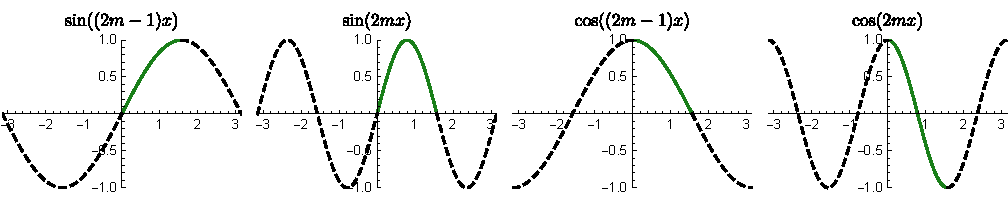
\includegraphics[width=0.8\textwidth]{figures/1.pdf}
    \caption{Графики функция при $m=1$ для Т4}
\end{figure}
И, аналогично, для $k=2$ (рис. 2). 
\begin{figure}[ht]
    \centering
    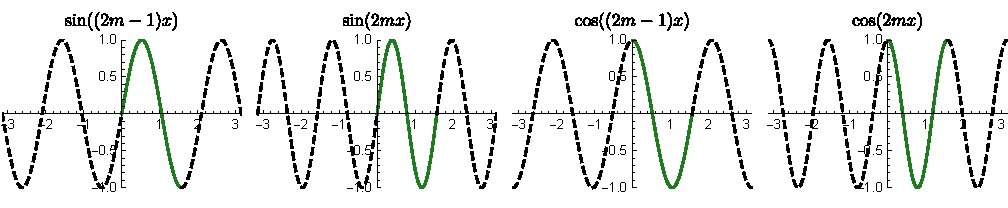
\includegraphics[width=0.8\textwidth]{figures/2.pdf}
    \caption{Графики функция при $m=2$ для Т4}
\end{figure}




\subsubsection*{Т5}

Аналогично Т4, рассмотрим полноту систем некоторых функция в пространстве $C[0, \pi/2]$. В частности покажем, что $\exists \tilde{x} \in C[0, \pi/2]$ и $\exists \varepsilon_0 \ \forall \tau_n$. Все синусы упираются в 0, выберем $\tilde{x}(t) = 1$, тогда
\begin{equation*}
    \|\tilde{x} - \tau_n\|_{\infty} = \sup_{x \in [0, \pi/2]} |\tilde{x}(t) - \tau_n(t)| \geq |\tilde{x} - \tau_n| = |\tilde{x}-\tau_n|(0) = 
    |1-0| = \varepsilon_0.
\end{equation*}
Получается, что ломаются все синусы и косинусы с <<нечётными дугами>> (достаточно взять $t=\frac{\pi}{2}$), что явно видно по построению. 

Итого, единственная хорошая система, -- $\cos(2k\, x)$. 
\subsubsection*{Т6. Функции Эрмита}

Приведем пример счетной системы фукций, полной в $L_2(\mathbb{R})$. В частности, воспользуемся функциями Эрмита:
\begin{equation*}
    \varphi_n (t) = c_n H_n(t) e^{-\frac{1}{2}t^2},
    \hspace{5 mm} 
    H_n (t) = e^{\frac{1}{2}t^2} \frac{d^n}{d t^n} e^{-\frac{1}{2} t^2}.
\end{equation*}
Утверждается, что это базис $L_2(\mathbb{R})$, докажем это. 

Есть система функций
\begin{equation*}
    \mathcal L = \{\varphi_n (t)\} = \{\rho(t) e^{-\frac{1}{2}t^2}, \ \rho \in \mathcal P\}. 
\end{equation*}
Так как $L_2$ -- гильбертово пространство, то достаточно проверить замкнутость системы, то есть показать, что $\mathcal L^\bot = \{0\}$. По определению:
\begin{equation*}
    f \in \mathcal L^\bot,
    \hspace{0.5cm} \Rightarrow \hspace{0.5cm}
    \int_{\mathbb{R}} f(t) t^n e^{-\frac{1}{2}t^2} \d t = 0,
    \hspace{5 mm} n \in \mathbb{N}. 
\end{equation*}
Рассмотрим преобразование Фурье:
\begin{align*}
    F\left[f(t)e^{-\frac{1}{2}t^2}\right](y) &= \int_{\mathbb{R}} \frac{\d t}{\sqrt{2\pi}} f(t) e^{-\frac{1}{2}t^2}, e^{-i y t} = 
    \int_{\mathbb{R}} \frac{\d t}{\sqrt{2\pi}} f(t) e^{-\frac{1}{2}t^2} 
    \sum_{n=0}^{\infty} \frac{(-iy t)^n}{n!} =\\
    &\overset{\encircled{!}}{=} 
    \sum_{n=0}^{\infty}  \frac{(-iy)^n}{n!} \int_{\mathbb{R}} \frac{\d t}{\sqrt{2\pi}} f(t) \underbrace{t^n e^{-\frac{1}{2}t^2}}_{=0 \text{\ по условию}} = 0,
\end{align*}
таким образом мы выяснили, что Фурье функции $\equiv 0$. 

Далее воспользуемся тем, что $f(t) e^{-\frac{1}{2}t^2} \in L_2\left(\mathbb{R}\right)$, а значит работает равенство Парсеваля:
\begin{equation*}
    \int_\mathbb{R} \bigg|f(t) e^{-\frac{1}{2}t^2}\bigg|^2 \frac{\d t}{2 \pi} = 
    \int_{\mathbb{R}} \big|F[\ldots](y)\big|^2 \d y = 0,
    \hspace{0.5cm} \Rightarrow \hspace{0.5cm}
    f(t) e^{-\frac{1}{2}t^2} = 0,
    \hspace{0.5cm} \Rightarrow \hspace{0.5cm}
    f(t) = 0,
\end{equation*}
по крайней мере кроме множества меры нуль. Таким образом функции эрмита составляют базис в $L_2$.



% \encircled{!} -- теоерма Фубини, объяснить, лемма Лебеша о мажорируемой сходимости


\subsubsection*{Т7}


Возьмём функцию, которая лежит в $L_2$, но не лежит в $
\overset{\vspace{-1pt}\scalebox{0.5}{$\circ$}}{C} [-\pi,\pi]$, например, ограничение $\sign x$. И рассмотрим
подпространство $V\subset \overset{\vspace{-1pt}\scalebox{0.5}{$\circ$}}{C} [-\pi,\pi]$, заданное ортогональностью к
ней, то есть заданное формулой
\[
\int_{-\pi}^0 f(x)\; dx = \int_0^\pi f(x)\; dx.
\]

Это $V$ есть замкнутое подпространство в $\overset{\vspace{-1pt}\scalebox{0.5}{$\circ$}}{C}[-\pi,\pi]$ и в нём
можно выбрать какую-то полную систему, и даже её ортогонализовать. Если
начать с тригонометрической системы, то косинусы и чётные синусы и так
лежат в $V$, нечётные синусы надо будет подправить, скомбинировав их с
$\sin x$, а потом ещё ортогонализовать (что может быть неприятно).

В итоге, система не может быть полна в $\overset{\vspace{-1pt}\scalebox{0.5}{$\circ$}}{C}[-\pi,\pi]$, так как её
линейные комбинации не выходят за пределы $V$. А что касается
замкнутости, то переходя в гильбертово $L_2$ видно, что ортогональное
дополнение к замыканию образа $V$ в гильбертовом пространстве одномерно
и натянуто на этот вот $\sign x$, который разрывен и не лежит в образе
$\overset{\vspace{-1pt}\scalebox{0.5}{$\circ$}}{C}[-\pi,\pi]$. Так что замкнутость в терминах $\overset{\vspace{-1pt}\scalebox{0.5}{$\circ$}}{C}[-\pi,\pi]$ есть.

\subsection{Банаховы пространства и их двойственные}





\subsubsection*{Т8}

Здесь, и далее $p(x) = \|x\|$, $q(x) = \|x\|'$. Нормы \textit{эквивалентны}, если
\begin{equation*}
    \exists m, M \ \colon  \ m p(x) \leq q(x) \leq M p(x) \  \ \forall x.
\end{equation*}
% ульянов бахвалов -- Rn, 3,99
% Кудрявцев, том 3
% базис Гамиля есть всегда!
Так вот, всегда есть $\{e_k\}_{k=1}^n$ базис Гамиля, такой что $x = \sum_{k=1}^n x_k e_k$, где естественно ввести норму вида
\begin{equation*}
    p(x) = \sum_{k=1}^n |x_k|.
\end{equation*}
Пусть $q(x)$ -- ещё одна норма на $X$, в качестве мажоранты выберем $M = \max\limits_{i=1, \ldots, n}  q(e_i)$.
Теперь можем оценить сумму сверху:
\begin{equation*}
    q(x) = q\left(
        \sum_{k=1}^n x_k e_k
    \right) \leq \sum_{k=1}^{n} |x_k| q(e_k) \leq M \cdot p(x).
\end{equation*}
И оценить снизу:
\begin{equation*}
    |q(x) - q(y)| \leq q(x-y) \leq M \cdot p (x-y),
\end{equation*}
вообще это значит, что $q$ -- липшецев функционал, -- непрерывный функционал на $X$ с нормой $p$, а тогда и $q(x)$ непрерывный функционал $X$ с нормой $p(x)$. 


\begin{to_lem}
    Шары в пространстве компактны тогда, и только тогда, когда $\dim X < + \infty$.
\end{to_lem}

Рассмотрим сферу $S = \{x \in X \mid p(x) = 1\}$ -- компакт. Но мы знаем, что непрерывный функционал на компакте достигает своего миниимума:
\begin{equation*}
    \min_{x \in S} q(x) = \min_{p(x)=1} q(x) = m > 0.
\end{equation*}
Тогда на сфере $S$ верно, что $q(x) \geq m$. Тогда в $X$ $q(x) \geq m \cdot p(x)$. Действительно,
\begin{equation*}
    q(tx) = |t|q(x), \ \  p(tx) = |t| \, p(x), \hspace{0.5cm} \Rightarrow \hspace{0.5cm}
    q(tx) = \frac{p(tx)}{p(x)} q(x) \geq m\, p(tx).
\end{equation*}
Собственно, $m p(x) \leq q(x) \leq M \cdot p(x)$,  $Q.\, E.\, D.$




\subsubsection*{Т9. Пространство \texorpdfstring{$c$}{с}}

Пространство состоит из некоторых бесконечномерных <<векторов>>  (последовательностей):
\begin{equation*}
    x = \big(x(1), x(2), \ldots, x(k), \ldots\big),
    \hspace{5 mm}
    \bigg|
        \lim_{k \to \infty} x(k)
    \bigg| < + \infty.
\end{equation*}
Норма определена, как
\begin{equation*}
    p(x) = \|x\|_c = \sup_{k \in \mathbb{N}} |x(k)| = \|x\|_{\infty}.
\end{equation*}
Докажем, что это пространство является банаховым, а именно полноту по $\|\cdot\|_{\infty}$ норме. 

Рассмотрим последовательность $x_n$, где 
\begin{equation*}
    x_n = (x_n (1), \ldots, x_n(k), \ldots).
\end{equation*}
Глобально хотим показать, что
\begin{equation*}
    \forall \varepsilon > 0 \ \ 
    \exists N(\varepsilon) \in \mathbb{N} \ \ 
    \forall n \geq N(\varepsilon) \ \ 
    \forall l \in \mathbb{N} \ \  \ 
    \|x_{n+l} -x_{n}\|_{\infty} = \sup_{k \in \mathbb{N}} |x_{n+l} (k) - x_n (k)| < \varepsilon.
\end{equation*}
Попробуем через это продраться: из сходимости следует, что
\begin{equation*}
    \forall k \in \mathbb{N} \ \ |x_{n+l} (k) - x_n (k) | < \varepsilon.
\end{equation*}
Здесь можем выделить $(x_n(k))_{n \in \mathbb{N}}$ -- числовая фундаментальная в $\mathbb{R}$. 
По критерию Коши:
\begin{equation*}
    \forall k \in \mathbb{N} \ \ 
    \lim_{n \to \infty} x_n (k) = y(k) \in \mathbb{R},
\end{equation*}
уставнавливается покомпонентая сходимость. 
Теперь рассмотрим
\begin{equation*}
    \sup_{k\in \mathbb{N}} |x_n (k) - y(k)| = \|x_n - y\|_{\infty} < \varepsilon,
\end{equation*}
что автоматически означает, что $\exists y$ такой, что
\begin{equation*}
    \lim_{n \to \infty} x_n  = y.
\end{equation*}

Следующий этап -- показать, что
\begin{equation*}
    \exists \lim_{k \to \infty} y(k) \in \mathbb{R},
\end{equation*}
то есть показать полноту пространства:
\begin{align*}
    |y(k+q)-y(k)| 
    &= |y(k+q) - x_n (k+q) + x_n (k+q) - x_n (k) + x_n (k) - x_n (k)|\\
    &\leq |y(k+q)-x_n (k+q)| + |y(k) - x_n (k)| + |x_n (k+q) - x_n (k)| \\
    & < \varepsilon/3 + \varepsilon/3 + \varepsilon/3 = \varepsilon.
\end{align*}
Таким образом мы доказали полноту пространства\footnote{
    \red{$c_0, c_{00}, l_\infty$ -- банаховы ли?
    $\encircled{!}$: $c_0$ (сходящиеся к $0$), $c_{00}$ (финитные), $l_\infty$ (ограниченные). 
    }  
} . 


\subsubsection*{Т10. Критерий Йордана-фон Неймана}

% \begin{to_def}
%     Если норма в банаховом пространстве $E$ порождается положительно определенным скалярным произведением 
%     \begin{equation*}
%         \|x\| = \sqrt{(x, x)},
%     \end{equation*}
%     то $E$ называется \textit{гильбертовым пространством}.
% \end{to_def}

Хочется понять, можно ли ввести на пространстве $C[a,b]$ скалярное произведение так, что норма пространства будет получаться из этого скадяного произведения.

\begin{to_thr}[критерий Йордана-фон Неймана]
    Норма $\|\circ\|_X$ порождается скалярным произведением тогда, и тоглько тогда, когда
    $\|\circ\|_X$ удовлетворяет правилу параллелограмма:
    \begin{equation*}
        \forall x, y \in X \ \ \ 
        \|x+y\|^2_X + \|x-y\|^2_X = 2 \|x\|_X^2 + 2 \|y\|_X^2.
    \end{equation*}
\end{to_thr}

\noindent
Выберем $C[0, \pi/2]$, и $x(t) = \cos t$, $y(t) = \sin t $. Заметим, что
\begin{equation*}
    \|x\|_{\infty} = \|y\|_{\infty} = 1,
    \hspace{5 mm}
    \|x+y\|_{\infty} = \sqrt{2}, \hspace{5 mm} \|x-y\|_\infty = 1,
    \hspace{5 mm} 
    2+1 \neq 2+2,
\end{equation*}
таким образом пространство не гильбертово.



\subsubsection*{Т11. Поиск функционала}

Далее будем обозначать за $\mathcal D(A)$ область определения оператора $A$, и $\mathcal R (A)$ -- область значений. Оператор действует $A \colon  X \mapsto Y$, где $X$ и $Y$ -- линейные нормированные пространства. 

\begin{to_def}
    Говорится, что линейный оператор $A \colon  X \mapsto Y$ \textit{непрерывен} а точка $x \in \mathcal D(A)$, если $\forall \, \{x_n\}_{n=1}^{\infty} \subset \mathcal D(A)$, сходящейся к $x$ в $X$, $A x_n \to A x$ в $Y$. Оператор \textit{глобально непрерывен}, если он непрерывен $\forall x \in \mathcal D(A)$. 
\end{to_def}

\begin{to_lem}
    Для того, чтобы линейный оператор $A$ был непрерывен на всей $\mathcal D(A)$, необходимо и достаточно, чтобы он был непрерывен в нуле.
\end{to_lem}

\begin{to_def}
    Линейный оператор $A \colon  X \mapsto Y$ называется \textit{ограниченным}, если $\exists C >0 \colon  \|A x\|_Y \leq C \cdot \|x\|_X$ $\forall x \in \mathcal D(A)$. Наименьшее из чисел $C$ называется \textit{нормой} оператора $A$ и обозначается $\|A\|$. 
\end{to_def}

\begin{to_lem}
    Для того, чтобы линейный оператор был ограниченным, необходимо и достаточно, чтобы он переводил всякое ограниченное в $X$ множество, в ограниченное в $Y$. 
\end{to_lem}

\begin{to_thr}[]
    Оператор $A$ непрерывен тогда, и только тогда, когда он ограничен.
\end{to_thr}

\begin{to_thr}[о норме линейного оператора]
    Верно, что 
    \begin{equation*}
        \|A\| = \sup_{\|x\|=1} \|Ax\| = \sup_{\|x\|\neq 0} \frac{\|Ax\|}{\|x\|}.
    \end{equation*}
\end{to_thr}


Найдём норму функционала
\begin{equation*}
    A \colon  f \mapsto \sum_{k=0}^N (-1)^k f\left(\frac{k}{N}\right),
\end{equation*}
на пространстве $C[0,1]$. 


Вообще нормированным пространством мы называем пару вида $(X, \|\circ\|_X)$. И пусть есть некоторый непрерывный ограниченный оператор из $X$ в $Y$. Если $Y = \mathbb{C}(\mathbb{R})$, 
\begin{equation*}
    A = F \colon  X \to \mathbb{C}(\mathbb{R}),
\end{equation*}
то  $A$ называют \textit{функционалом}. Выберем в качетсве $X = C[0, 1]$, а в качетсве $F \colon C[0, 1] \mapsto \mathbb{C}(\mathbb{R})$.
Функционал вида
\begin{equation*}
    F[f] = \sum_{k=0}^{n}(-1)^k f\left(\frac{k}{n}\right).
\end{equation*}
Что есть норма функционала? Норма функционала есть
\begin{align*}
    \|F\| 
    &= \sup_{\|f\|_{\infty} \leq 1} |F[f]|  
    = \sup_{\|f\|_{\infty} = 1} |F[f]| 
    = \inf \{
        L > 0 \mid |F[f]| \leq L\|f\|_\infty
    \}, 
    \hspace{5 mm} \forall f \in C[0, 1].
\end{align*}
\texttt{Глобально, это доказывается, например, в Константинове очень подробно.} 

\texttt{Всегда легко сверху ограничить.} Тривиальный шаг:
\begin{equation*}
    |F[f]| = \bigg|
        \sum_{k=0}^{n} (-1)^k f\left(
            \frac{k}{n}
        \right)
    \bigg| \leq \sum_{k=0}^{n} \bigg|
        f\left(\frac{k}{n}\right)
    \bigg| \leq \sum_{k=0}^{n} \sup_{x \in [0,1 ]} |f(x)| = (n+1) \cdot \|f\|_{\infty}.
\end{equation*}
Продолжаем, 
\begin{equation*}
    \frac{|F[f]|}{\|f\|_{\infty}} \leq n + 1,
    \hspace{0.5cm} \Rightarrow \hspace{0.5cm}
    \|F\| = \sup_{\|f\|_{\infty} = 1} |F[f]| \leq n+1.
\end{equation*}
Теперь выберем функцию $f_s(x) = f(k/n) = (-1)^k$. На ней мы действительно достигаем супремум, тогда
\begin{equation*}
    \|F\| = |F[f_s]| = n+1.
\end{equation*}
Таким образом нашли норму оператора. 

В более общем случае можем показать, что
\begin{equation*}
F[f] = \sum_{k=1}^{n}  c_k x(t_k),
\hspace{5 mm} 
    |F[f]| \leq \sum_{k=1}^{n} |c_k| \cdot \|f\|_{\infty},
    \hspace{0.5cm} \Rightarrow \hspace{0.5cm}
    \|F\| \leq \sum_{k=1}^{n} |c_k|.
\end{equation*}
Далее, определив схожим образом непрерывную функцию $\tilde{f}$, равную $\sign c_k$ в $t=t_k$ увидим, что $\|\tilde{f}\|=1$, 
\begin{equation*}
    \|F[\tilde{f}]\| \geq |F[\tilde{f}]| = \sum_{k=1}^{n}  |c_k|,
\end{equation*}
таким образом решили чуть более общую задачу. 







\subsubsection*{Т12}


Пусть функция $g$ непрерывна на $[a, b]$. Найдём норму линейного отображения $M_g \colon L_2[a, b] \mapsto L_2[a,b]$, где $A_g(f) = [f]$ -- мультипликативный оператор. Здесь $X=Y=L_2[a,b]$. 

По опредению, норма оператора $\|A_g\| = \sup_{\|f\|_X = 1} \|A_g [f]\|_Y$. Аналогично, ищем ограничение сверху:
\begin{equation*}
    \|A_g [f]\|_2^2 = \|gf\|_2^2 = \int_{[a, b]} |gf|^2 (x) \mu(\d x) \leq 
    \int_{[a, b]} \left\{
        \sup_{x\in[a,b]} |g(x)|
    \right\}^2 |f(x)|^2 \mu(\d x).
\end{equation*}
Вынесенный супремум позволит записать:
\begin{equation*}
    \|A_g[f]\|_2^2 \leq \|g\|_\infty^2 \|f\|_2^2,
    \hspace{0.5cm} \Rightarrow \hspace{0.5cm}
    \|A_g\| = \sup_{\|f\|_2=1} \|A_g[f]\|_2 \leq \|g\|_\infty.
\end{equation*}
Далее покажем, что норма не достигается, но сколь угодно близко приближается.


Есть функция 
\begin{equation*}
    \sup_{x\in[a,b]} |g(x)| = |g(c)|,
\end{equation*}
есть некоторая $f_\varepsilon \in L_2[a, b]$ вида
\begin{equation*}
    f(x) = \left\{\begin{aligned}
        &\alpha_\varepsilon, &x\in[c-\varepsilon, c+\varepsilon], \\
        &0, &x\notin[c-\varepsilon, c+\varepsilon],
    \end{aligned}\right.
    \hspace{0.5cm} \Rightarrow \hspace{0.5cm}
    \|f_\varepsilon\|_2^2 = \int_{[c-\varepsilon, c+\varepsilon]} \hspace{-10mm} \alpha_\varepsilon^2 \mu(d x) =
    \alpha_\varepsilon^2 \cdot 2 \varepsilon = 1,
    \hspace{5 mm} 
    \alpha_\varepsilon = \frac{1}{\sqrt{2\varepsilon}}.
\end{equation*}
В таком случае рассмотрим
\begin{equation*}
    \|A_g [f_\varepsilon]\|_2^2 = \|g f_\varepsilon\|_2^2 = \alpha_\varepsilon^2 \int_{[c-\varepsilon, c+\varepsilon]} \hspace{-10mm} |g(x)|^2 \mu(dx) = \alpha_\varepsilon^2 \cdot 2 \varepsilon |g(x_{c,\varepsilon})|^2 \underset{\varepsilon\to 0}{\to} \|g\|_\infty^2,
\end{equation*}
в силу непрерывности $g$, по теореме о среднем.


Можно пойти другим путем, по определению:
\begin{equation*}
    \forall \varepsilon \in (0, \|g\|_\infty), \hspace{5 mm} 
    \exists x_\varepsilon \subseteq [a, b] \ 
    g(x) \geq \|g\|_\infty - \varepsilon,
\end{equation*}
почти всюду на $X_\varepsilon$. Выберем $h(x)$ вида
\begin{equation*}
    h(x) = \sign g(x) \ \cf{X_\varepsilon} (x),
    \hspace{5 mm} 
    \|h_\varepsilon\|_1 = \|h_\varepsilon\|_2 = \mu(X_\varepsilon), 
\end{equation*}
тогда верно, что
\begin{equation*}
    \|A_g\| \geq \|A_g [h_\varepsilon]\|_1 \cdot \|h_\varepsilon\|_1 = \int_{[a, b]} |g(x)| \cf{X_\varepsilon} (x) \mu(\d x) \geq \left(
        \|g\|_{\infty} - \varepsilon
    \right) \chi \mu(X_\varepsilon),
    \hspace{0.5cm} \Rightarrow \hspace{0.5cm}
    \|A_g\| = \|g\|_\infty.
\end{equation*}
Аналогично в $L_2$:
\begin{equation*}
    \|A_g\|^2 \geq \||g| \cf{X_\varepsilon}\|_2^2 \cdot \|h_\varepsilon\|_2^2 \geq \|g\|_\infty^2 \mu^2(X_\varepsilon),
\end{equation*}
что приводит такому же результату. 


\subsubsection*{Т13}


Сначала  найдём норму оператора $F$, откуда уже получим значение нормы для $J$, где
\begin{equation*}
    F[f] = \int_a^b g(t) f(t) \d t,
    \hspace{5 mm} 
    J[f] = \int_{a}^{b} K(x, y) f(y) \d y,
\end{equation*}
где $g\in C[a,b]$, а $F, \ J$ -- линейные функционалы на $C[a, b]$. 


\textbf{Первая часть}. Функционал $F$ ограничен в силу
\begin{equation*}
    |F[f]| \leq \int_{a}^{b} |g(t) |f(t)| \d t \leq \|f\|_\infty \cdot \int_{a}^{b} |g(t)| \d t.
\end{equation*}
Далее выберем произвольное $\varepsilon  > 0$. По \textit{теореме Кантора} найдётся такое разбиение отрезка $[a, b]$ точками $a=t_0 < t_1 < \ldots < t_n = b$, что колебание $\omega_i(g)$ функции $g$ на $i$-ом отрезке $\Delta_i = [t_{i-1}, t_i]$ удовлетворяет неравенствам 
\begin{equation*}
    \omega_i(g) < \varepsilon, \hspace{5 mm} i = 1,\, 2,\, \ldots,\, n.
\end{equation*}
Разобьём все $\Delta_i$ на две группы. В первую группу отнесем те отрезки, на которых $g$ сохраняет знак. Пусть это будут отрезки $\Delta_1',\ldots,\Delta_r'$. Вторую группу $\Delta_1'', \ldots, \Delta_s''$ образуют отрезки, на которых $g$ меняется знак. В каждом промежутке второго типа существует точка, в которой $g$ обращается в нуль. Ввиду установленных неравенств там $|g(t)|<\varepsilon$. 

На промежутках первого типа положим $\tilde{f}(t) = \sign g(t)$, в остальных точках $\tilde{f}(t)$ -- линейная непрерывная функция, удовлетворяющая неравенству $|\tilde{f}| \leq 1$. Тогда $\|\tilde{f}\|=1$, и 
\begin{align*}
    \|F\| &= \sup_{\|f\|=1} |F[f]| \geq |F[\tilde{f}]| = \bigg|
        \int_a^b g(t) \tilde{f}(t) \d t
    \bigg| = 
    \bigg|
        \sum_{k=1}^{r} \int_{\Delta'_k} |g(t)|\d t + \sum_{i=1}^{s} \int_{\Delta''_i} g(t) \tilde{f}(t) \d t
    \bigg| 
    \geq \\ &\geq
    \sum_{k=1}^{r}  \int_{\Delta'_k} |g(t)| \d t - 
    \sum_{i=1}^{s} \int_{\Delta_i''} = \int_a^b |g(t)| \d t - 
    2 \sum_{i=1}^{s}  \int_{\Delta''_i} |g(t)| \d t \geq \int_{a}^{b} |g(t)| \d t - 2 \varepsilon \cdot \mu[a, b],
\end{align*}
что ввиду произвольности $\varepsilon$ означает, что $\|F\|\geq \int_a^b |g(t)| \d t$, что вместе со знанием супремума позволяет утверждать: $\|f\|=\int_a^b |g(t)| \d t$.


\textbf{Вторая часть}. Переходим к поиску нормы $J$:
\begin{align*}
    \|J[f]\| = \sup_{t\in[a, b]} \bigg| 
        \int_{a}^{b} K(t, s) f(s) \d s
    \bigg| \leq \sup_{t\in[a, b]} \int_{a}^{b}  |K(t, s)| \cdot |f(s)| \d s \leq 
    \|f\| \cdot \sup_{t\in[a, b]} \int_{a}^{b} |K(t, s)| \d s,
\end{align*}
таким образом, по определению
\begin{equation*}
    \|J\| \leq \sup_{t\in[a, b]} \int_{a}^{b} |K(t, s)| \d s \overset{\mathrm{def}}{=}  M.
\end{equation*}
Так как ядро $K$ непрерывно, то непрерывен и интеграл $\int_a^b |K|\d s$, поэтому $\exists t_0 \in [a, b]$ такой, что $M = \int_{a}^{b} |K(t_0, s)|\d s$. 

Как было показано в первой части, $q(x) = \int_{a}^{b}  |K(t_0, s)| f(s) \d s$ -- линейный непрерывный функционал на $C[a, b]$ с нормой равной $M$. Таким образом, выбирая $\tilde{f}$ так, чтобы $\sign \tilde{f(s)} = \sign K(t_0, s)$ может утверждать, что супремум достигается, и 
\begin{equation*}
    \|J\| = M = \sup_{t\in[a, b]} \int_{a}^{b}  |K(t, s)| \d s.
\end{equation*}



\begin{to_thr}[Теоремма Бэра для открытых множеств]
    Счётное семейство открытых всюду плотных подмножеств банахова пространства имеет непустое пересечение.
\end{to_thr}

\begin{to_thr}[Теорема Бэра для замкнутых множеств]
    Если банахово пространство $E$ покрыто счётным семейством замкнутых множеств, то одно из них имеет непустую внутренность. 
\end{to_thr}

\subsubsection*{Т14}

Докажем, что алгебраический базис бесконечномерного банахова пространства не может быть счётным. 

Вводился алгебраический базис Гамиля $\{e_\alpha\}_{\alpha\in A}$, где $\forall x \in E$ представляется в виде
$x \ \sum_{k=1}^{n}  x_k e_{\alpha_k}$. Получается, что нужно показать, что в бесконечномерном банаховом пространстве такой базис не может быть счётным: докажем от противного.


Пусть $\{e_n\}_{n\in \mathbb{N}}$, тогда пространство описывется, как
\begin{equation*}
    E_n = \left\{
        \sum_{k=1}^{n} x_k e_k \mid x_1, \ldots, x_k \in \mathbb{R}
    \right\} = \langle E_1, \ldots, e_n \rangle,
    \hspace{0.5cm} \Rightarrow \hspace{0.5cm}
    E = \bigcup_{n\in \mathbb{N} } E_n.
\end{equation*}
Но по теореме Бэра для замкнутых множеств $E$ не может быть счётным объединением нигде не плотных множеств.

Точнее, это было бы возможно, только с случае непустой внутренности одного из пространств $E_n$, что невозможно. 


% Мы знаем, что $E_n$ -- замкнуто, $E$ -- полно. Тогда, по следствию из теоремы Бэра,
% \begin{equation*}
%     \exists n_0 \in \mathbb{N} \colon \ \ E \subset E_{n_0}, 
% \end{equation*}
% что приводит к противоречию, в силу бесконечности $E$. 


\subsubsection*{Т15}

Приведем пример плотного в $X = C[a,b]$ банахова пространства, со счётным базисом. 

 
По теореме Вейерштрассе система степеней $A$ полна в $C[a, b]$, что равносильно тому, что линейная оболочка системы степеней $A$ плотна на $C[a,b]$. Таким образом, $A$ со счётным базисом, является ответом на задачу.

\begin{to_def}
    Последовательность элементов $\{e_n\}_{n\in \mathbb{N}}$ называется \textit{базисом} в пространстве\footnote{
Если линейное нормированное пространство имеет не более, чем счётный базис, то оно сепарабельно. Однако существуют сепарабельные банаховы пространства без базиса.
    }  $X$, если $\forall x \in X$ существует единственный набор $\{x_i\}_{i \in \mathbb{N}_0}$ таких, что сумма вида (не конечная не при каком $n$)
    \begin{equation*}
        x = \sum_{k=1}^{\infty} x_k e_k = \lim_{n \to \infty} \sum_{k=1}^{n} x_k e_k,
        \hspace{5 mm} \Leftrightarrow \hspace{5 mm} 
        \exists ! \{x_i\}_{i \in \mathbb{N}_0} \ 
        \forall \varepsilon > 0 \ 
        \exists N_\varepsilon \in \mathbb{N}_0 \ 
        \forall n \geq N_\varepsilon \ 
        \|x - \sum_{k=0}^{n} x_k e_k\|_X = \|x-S_n\| < \varepsilon.
    \end{equation*}
\end{to_def}

\begin{to_thr}[Теорема Банаха-Штейнгауза для линейных функционалов]
    Пусть семейство линейный функционалов $Y \subset E'$ ограничено в любой точке банахова пространства $E$, то есть для любого $x \in E$ множество чисел $\{\lambda(x) \mid \lambda \in Y\}$ ограничено. Тогда $Y$ ограничено в смысле нормы в $E'$. 
\end{to_thr}


% см. Конспект Карасева сразу после Банаха-Щтейнгауза

\subsubsection*{Т16}


\begin{to_thr}[Расходимость ряда Фурье в точке]
    Существует непрерывная $2\pi$-периодическая функция, ряд Фурье которой расходится в точке 0.
\end{to_thr}

\begin{proof}[$\triangle$]
На пространстве $\dot{C}[-\pi, \pi]$ непрерывных $2\pi$ -периодических функций с нормой $\|\cdot\|_C$ определим линейный функционал 
\begin{equation*}
    \lambda_n (f) = \int_{-\pi}^{\pi} f(t) D_n(t) \d t,
\end{equation*}
это значение $n$-й частичной суммы ряда Фурье в точке $0,\, T_n(f, 0)$. Можно заметить по определению нормы, что его норма равна
\begin{equation*}
    \|\lambda_n\| = \int_{-\pi}^{\pi} |D_n(t)| \d t.
\end{equation*}
Оценим интеграл модуля ядра Дирихле стандартным способом:
\begin{align*}
    I &= \int_{-\pi}^{\pi} \frac{|\sin(n+1/2)x|}{2 \pi |\sin x/2|} \d x \geq 
    \int_{-\pi}^{\pi} \frac{|\sin(n+1/2)x|}{\pi |x|} \d x =  \int_{-\pi(1+1/2)}^{\pi(1+1/2)} \frac{|\sin u|}{\pi |u|} \d u 
    \geq \\ &\geq 
    \int_{-\pi(1+1/2)}^{\pi(1+1/2)} \frac{\sin^2 u}{\pi |u|} \d u = \int_{-\pi(1+1/2)}^{\pi(1+1/2)} \frac{1-\cos 2u}{2\pi |u|}\d u \to 
    \int_{-\infty}^{\infty} \frac{1 - \cos 2 u}{2\pi |u|} \d u = + \infty,
    \hspace{5 mm} 
    n \to \infty.
\end{align*}
Получается, то нормы функционалов $\lambda_n$ при $n \to \infty$ не являются ограниченными. Следовательно, по теореме Банаха-Штейгауза, примененной в обратную сторону, для некоторой функции $f \in \dot{C}[-\pi, \pi]$ значения $\lambda_n (f) = T_n(f, 0)$ не будут ограничены, и, следоватеьно, расходятся при $n \to \infty$. 


\end{proof}
\subsubsection*{Т17}

Для последовательностей 
\begin{equation*}
    x = (x(1), \ldots, x(k), \ldots),
\end{equation*}
рассмотрим пространство вида
\begin{equation*}
    l_p = \{x \mid \|x\|_p \in \mathbb{R} \},
    \hspace{5 mm} 
    \|x\|_p = \l(
        \sum_{k=1}^{\infty} |x(k)|^p
    \r)^{1/p}.
\end{equation*}
Возьмём пространство $l_p$ как множество, но добавим норму из пространства $l_q$, где $\infty > q > p$. Покажем, что в таком <<дырявом>> пространстве не выполняется теорема Бэра и принцип равномерной ограниченности. 

Рассмотрим шар $A_n$ вида
\begin{equation*}
    A_n = \{x \in l_p \mid \|x\|_p \leq n\},
    \hspace{5 mm}
    l_p = \bigcap_{n=1}^{\infty} A_n.
\end{equation*}
Докажем от противного, что $A_n$ нигде не плотно. 

Пусть существует такой $R > 0$ и $x_0 \in A_n \colon B_R (x_0) \subset \cl A_n = A_n$. 
\begin{equation*}
    \forall x \in l_p \colon  \ \ \ 
    \rho_q (x, x_0) < R,
    \hspace{0.5cm} \Rightarrow \hspace{0.5cm}
    x \in A_n \hspace{0.5cm} \Rightarrow \hspace{0.5cm}
    \|x\|_p \leq n.
\end{equation*}
Рассмотрим некоторую последовательность
\begin{equation*}
    z(k) = \frac{R}{2} \frac{1}{\sum_{\kappa=1}^{\infty} \frac{1}{\kappa^{q/p}}} \frac{1}{k^{1/p}}.
\end{equation*}
Для начала,
\begin{equation*}
    \left(
        \sum_{k=1}^{\infty} (z(k))^{q}
    \right)^{1/q} = \|z\|_q = \frac{R}{2} < + \infty.
\end{equation*}
Далее, видим гармонический ряд
\begin{equation*}
    \sum_{k=1}^{\infty} (z(k))^p = + \infty,
    \hspace{0.5cm} \Rightarrow \hspace{0.5cm}
    \exists N  \colon  \sum_{k=1}^{N} (z(k))^p > (2n)^p.
\end{equation*}
Теперь рассмотрим набор <<частниных последовательностей>>
\begin{equation*}
    y(k) = \left\{\begin{aligned}
        &z(k), \ &k \leq N,
        &0, &k > N.
    \end{aligned}\right.
\end{equation*}
Теперь рассмотрим последовательность $h(k) = (x_0 + y) (k)$, для которой верно, что
\begin{enumerate}
    \item $\rho_q (h, x_0) = \|y\|_q \leq R/2$, откуда следует $\|h\|_p \leq n$.
    \item $\|h\|_p \geq \|y\|_p - \|x_0\|_p > 2n -n=n$, а тогда $\|h\|_p >n$, таким образом пришли к противоречию. 
\end{enumerate}

Полное пространство нельзя представить, как объединение нигде не плотных множеств, получается $l_p$ не полно. Осталось доказать, что $A_n$ замкнуто.

Пусть $t$ -- точка прикосновения. Тогда $\forall \varepsilon > 0$ найдётся 
\begin{equation*}
    \forall\varepsilon > 0 \ \ \ 
    \exists x_\varepsilon \in A_n \colon 
    \rho_q (t, x_\varepsilon) < \varepsilon,
    \hspace{0.5cm} \encircled{\Rightarrow} \hspace{0.5cm}
    \sum_{k=1}^{N} |t(k) - x_\varepsilon(k)|^q < \varepsilon
    \hspace{0.5cm} \Rightarrow \hspace{0.5cm}
    |t(k) - x_\varepsilon (k)|< \varepsilon^{1/q},
\end{equation*}
получается это правда и для
\begin{equation*}
    \encircled{\Rightarrow} \hspace{5 mm}
    \forall N \in \mathbb{N} \ 
    \left(
        \sum_{k=1}^{N} |t(k)|^p
    \right)^{1/p} \leq t(k) - x_\varepsilon (k) + x_\varepsilon(k) 
    \leq
    \left(
        \sum_{k=1}^{N} |t(k) - x_\varepsilon (k)|^p
    \right)^{1/p}  + 
    \left(
        \sum_{k=1}^{N} |x_\varepsilon (k)|^p
    \right)^{1/p} \leq 
    \left(
        N \varepsilon^{p/q}
    \right)^{1/p} + n,
\end{equation*}
что стремится к $n$ при $\varepsilon \to 0$. Таким образом $\|t\|_p \leq n$. 


И, наконец, докажем, что не выполняеся принцип равномерной ограниченности. Рассмотрим функционалы
\begin{equation*}
    F_n [x] = \sum_{k=1}^{n} x(k).
\end{equation*}
Верно, что
\begin{equation*}
    \forall x \in l_1 \ \ 
    |F_n[x]| \leq \|x\|_1.
\end{equation*}
По норме $\|\circ\|_2$ верно, что эти функционалы можно переписать в виде скалярного произведения $(x, e_n)$, где $e_n = (1, \ldots, 1, 0,\ldots,0,\ldots)$:
\begin{equation*}
    F_n [x] = (x, e_n) = \sum_{k=1}^{\infty}  x_{(k)} (e_n)_{(k)} = \sum_{k=1}^{n} x(k),
\end{equation*}
что является проявлением одной из теорем Рисса. Положив $x=e_n$ видим, что норма достигается и $\|F_n\| = n \to \infty$ при $n \to \infty$. Таким образом мы показали, что на таком пространстве не работает принцип равномерной сходимости. 




\subsubsection*{Т18}

Докажем, что в бесконечномерном банаховом пространстве $E$ единичный шар не явяется компактным. 


\begin{to_lem}[Лемма Рисса или лемма о перпендикуляре]
    Если $X_0$ -- замкнутое линейное подпространство в нормированом пространстве $X$, $X_0 \neq X$, тогда
    \begin{equation*}
        \forall \varepsilon > 0, \ \exists x_\varepsilon \in X \colon \|x_\varepsilon\| = 1,
        \hspace{5 mm} 
        \|x_\varepsilon - y\| \geq 1 - \varepsilon \ \ \forall y \in X_0.
    \end{equation*}
\end{to_lem}

\begin{proof}[$\triangle$]
    Найдётся $z \in X \backslash X_0$, положим $\delta = \inf\{
        \|z - u\| \mid y \in X_0
    \} > 0$.
    Тогда выберем
    \begin{equation*}
        \varepsilon_0 > 0 \colon  \frac{\delta}{\delta+\varepsilon_0} > 1 - \varepsilon,
    \end{equation*}
    выберем $y_0 \in X_0$ такой, что $\|z - y_0\| < \delta + \varepsilon_0$.

    Далее, считая
    \begin{equation*}
        x_\varepsilon = \frac{z-y_0}{\|z-y_0\|}, \  \ \forall y \in X_0.
    \end{equation*}
    Теперь оценим
    \begin{equation*}
        \|x_\varepsilon - y\| = \frac{1}{\|z-y_0\|} \|z-y_0-\|z-y_0\|y\| \geq \frac{\delta}{\delta+\varepsilon_0} > 1 - \varepsilon.
    \end{equation*}
    Заметим, что
    \begin{equation*}
        v = y_0 + \|z-y_0\| y \in X_0,
        \hspace{0.5cm} \Rightarrow \hspace{0.5cm}
        \|z-v\| \geq \delta.
    \end{equation*}
\end{proof}



\begin{to_con}
    В $\forall X$  (бесконеномерном, нормированном пространстве) $\exists (x_n) \colon  \|x_n\| = 1$ и
    $\|x_n - x_k\| \geq 1$, $n \neq k$.
    Как следставие все шары $R > 0$ в $X$ некомпактны. 
\end{to_con}

\begin{proof}[$\triangle$]

Всякое бесконечное подмножество компакта имеет предельную точку. 
Последовательность $x_n$ строится по индукции с помошью леммы Рисса. 

\end{proof}




\begin{to_thr}[Теорема Хана-Банаха]
    Пусть $E$ -- банахово пространтво, $F \subset E$ -- его линейное подпространство. Тогда всякий ограниченный линейный функционал $\lambda \in \mathbb{F'}$ продолжается до линейногофункционала на всём $E$ без увеличения его нормы. 
\end{to_thr}

\begin{to_con}
    Для всякого банахова пространства $E$ и его ненулевого элемента $x \in E$ найдётся $\lambda \in E'$, такой что $\|\lambda\|=1$ и $\lambda[x] = \|x\|$.
\end{to_con}

\begin{to_con}
    Естественное отображение банахова пространства в двойственное к его двойственному (второе двойственное) 
    \begin{equation*}
        E \mapsto E'',
        \hspace{5 mm} 
        x \mapsto \left(\lambda \mapsto \lambda(x)\right)
    \end{equation*}
    является вложением, сохраняющим норму. 
\end{to_con}


\begin{to_thr}[Теорема Радона-Никодима в $\mathbb{R}^n$]
    Пусть неотрицательная конечная борелевская мера $\mu$ на $\mathbb{R}^n$ абсолютно непрерывна относительно меры Лебега. Тогда у меры $\nu$ есть плотность, то есть борелевская $f \geq 0$, такая что для всякого борелевского $X$ $\nu(X) = \int_X f(x) \d x$. 
\end{to_thr}



\subsubsection*{Т19}

Выведем из теоремы Хана-Банаха, что всякое конечномерное подпространство $V$ в банаховом постранстве $E$ имеет замкнутое дополнение $W \subseteq E$, такое что $E = V \oplus W$. 

\begin{to_thr}[]
    Для всякого ненулевого элемента $x$ нормированного пространства $X$ найдётся такой функционал $l$, что $\|l\|=1$ и $l[f]=\|f\|$. 
\end{to_thr}

\begin{proof}[$\triangle$]
На одномерном пространствеЮ порожденном $x$Ю положим $l_0(tx) = t \|x\|$. Тогда $l_0 (x) = \|x\|$ и $\|l_0\|$ =1. Остается продолжить $l$ на $x$ с сохранением нормы. 
\end{proof}

Из этой теоремы можно получить, что в случае бесконечномерного пространства $X$ для всякого $n$ найдутся такие векторы $x_1, \ldots, x_n \in X$ и функционалы $l_1, \ldots, l_n \in X^*$, что $l_i (x_j) = \delta_{ij}$. В частности поэтому, сопряженное пространство тоже бесконечномерно. 

\begin{to_con}
    Пусть $X_0$ -- конечномерное подпростанство нормированного пространства $X$. Тогда $X_0$ топологически дополняемо в $X$, т.е. существует такое замкнутое линейное подпространство $X_1$, что $X$ является прямой алгебраической суммой $X_0$ и $X_1$, а естественные алгебраические проекции $P_0$ и $P_1$ на $X_0$ и $X_1$ непрерыны. 
\end{to_con}

\begin{proof}[$\triangle$]
    \textit{Можно} найти базис $x_1, \ldots, x_n$ пространства $X_0$ и элементы $l_i \in X^*$ с $l_i (x_j) = \delta_{ij}$. Положим
    \begin{equation*}
        X_1 \overset{\mathrm{def}}{=}  \bigcap_{i=1}^{n} \Ker l_i,
        \hspace{5 mm} 
        P_0 [x] \overset{\mathrm{def}}{=} \sum_{i=1}^{n} l_i (x) x_i,
        \hspace{5 mm} 
        P_1[x] \overset{\mathrm{def}}{=} x - P_0 x.
    \end{equation*}
    Для всякого $j$ имеем $P_0 [x_j] - l_j (x_j) x_j = x_j$. В таком контексте становится понятно, что $P_0 |_{X_1} = 0$, и $X_0 \cap X_1 = \{0\}$, $X = X_) \oplus X_1$, ибо $x - P_0 x \in X_1$ ввиду равенств $l_j (x-P_0 x) = l_j(x) - l_j (x) l_j(x_j) = 0$. Непрерывность $P_0$ и $P_1$ понятна из опредления, более того сопадают с алгебраическими проектированиями на $X_0$ и $X_1$.
\end{proof}




\subsubsection*{Т20}


Приведем пример замкнутого в топологии нормы множества $X \subset E'$ (двойственное к некоторому банахову пространству), которое не замкнутое в его *-слабой топологии. 


Ответ -- \textit{сфера}, докажем это. Покажем, что для $X \subset E'$ $\cl X = X$ и $w. \cl X \neq X$. Что есть сфера? Сфера есть
\begin{equation*}
    S = \{f \in E' \mid \|f\| = 1\}, 
    \hspace{5 mm} \cl S = S, 
    \hspace{5 mm} w. \cl S = \bar{B},
    \hspace{5 mm} 
    \bar{B} = \{F \in E' \mid \|f\|\leq 1\}.
\end{equation*}
Введём дополнение $S_C \overset{\mathrm{def}}{=} E\backslash S$, и покажем, что оно открыто. 


Выберем $g \in S_c$ с $\|g\|<1$ и $\varepsilon = 1- \|g\|> 0$. Пусть $h \in B_\varepsilon(g)$, более того
\begin{equation*}
    \|h\| = \|g + h - g\| \leq \|g\| + \|h-g\| < 1,
    \hspace{0.5cm} \Rightarrow \hspace{0.5cm}
    B_\varepsilon (g) \subseteq S_c. 
\end{equation*}
Далее, пусть $g \in S_c$ и $\|g\|>1$, тогда $\varepsilon = \|g\|-1 > 0$. Выберем $h \in B_\varepsilon (g)$, тогда 
\begin{equation*}
    \|g\| =  \|h+g-h\| \leq \|h\| + \|g-h\|,
    \hspace{0.5cm} \Rightarrow \hspace{0.5cm}
    \|h\| \geq \|g\|-(\|g\|-1) = 1,
\end{equation*}
получается $\|h\| > 1$ и $B_\varepsilon (g) \subseteq S_c$. Таким образом $S_c$ открыто, $S$ замкнуто. 


Докажем теперь, что $w, \cl S = \bar{B}$. Во-первых $\forall g_0 \notin B$ верно, что
\begin{equation*}
    \|g_0\| > 1,
    \hspace{5 mm} 
    \exists x_0 \in E, \ 
    \exists \varepsilon_0 > 0 \ 
    \forall g \in U_{x_0, g_0, \varepsilon_0} \ \ \|g\|>1,
    \hspace{0.5cm} \Rightarrow \hspace{0.5cm}
    w.\cl S \subseteq B. 
\end{equation*}
В чатсности, покажем, что
\begin{equation*}
    \|g\| \geq |g[x_0]| = |g[x_0] - g_0[x_0] + g_0[x_0]| \geq 
    |g_0[x_0]| - |g[x_0] - g_0[x_0]|,
\end{equation*}
что уже можно сделать строго больше:
\begin{equation*}
    \|g\| > |g_0 [x_0]| - \varepsilon_0 = 1,
\end{equation*}
где $\varepsilon_0 = |g_0[x_0]|-1$. 


Пусть теперь $\forall$ фиксированного $g_0 \in \bar{B}$ с $\|g_0\|<1$. Тогда 
\begin{equation*}
    \exists U(g_0) \colon  g_0 \in \bigcap_{k=1}^N U_{x_k, g_k, \varepsilon_k} \subset U(g_0).
\end{equation*}
Утверждается, что существует ненулевой $g$ такой, что $\forall t \in \mathbb{R}$ с $g_0 + t g \in U(g_0)$. 

Осталось построить цилиндрическое множество по которому <<прогуляемся>> до  нужной нам области.  Пусть
\begin{equation*}
    \varphi(t) = \|g_0 + tg\| \in C(\mathbb{R}),
    \hspace{5 mm} 
    |\varphi(t_1) - \varphi(t_2)| \leq |t_1 - t_2|  \cdot \|g\|.
\end{equation*}
Понятно, что $\varphi(0) = \|g_0\| < 1$. Тогда $\varphi(t) \geq |t| \cdot \|g\|-\|g\|_0 \to \infty$ при $t \to \infty$. По теореме о промежуточных значениях непрерывной функции
\begin{equation*}
     \exists t_0 \in \mathbb{R} \colon  \varphi(t_0) = 1,
     \hspace{0.5cm} \Rightarrow \hspace{0.5cm}
     g_0 +t_0 g \in S.
 \end{equation*} 
 Получается, что взяв точку из шара, и взяв её слабую окрестность, мы находим непустое пересечение этой окрестности со сферой. Из этого следует, что $g_0 \in w. \cl S$, а тогда и $\bar{B} \subseteq w. \cl S$, которое содержится в замкнутом шаре. Вывод: $\bar{B} = w. \cl S$. 







\subsubsection*{Т21}

Докажем, что $*$-слабой топологии $E'$ компактность некоторого множества влечет его замкнутость. 

\begin{to_lem}
    Слабая топология хаусдорфова.
\end{to_lem}


Пусть $K$ -- компакт в ХТП $X$. Пуcть $x \in X \backslash K$. Для $\forall y \in K$ $\exists U_y,\, V_y$ (открытые) такие, что $U_y \cap V_y = \varnothing$, где $x \in U_y$ и $y \in V_y$. 

Рассмотрим систему $S = \left\{V_y \mid y \in K\right\}$
-- открытое покрытие компакта $K$. Также $S_0 = \{V_y \mid y \in F\}$, $F$ -- конечное подмножество $K$ (т.к. $K$ -- компакт). 

Рассмотрим множество $U = \cap_{y\in F} U_y$ -- открытая окрестность точки $x$. Утверждается, что $U \cap K = \varnothing$. Перебирая все точки $x \in K$ получаем доказательство исходного утверждения.  
\subsubsection*{Т22}


Хочется найти такое топологическое пространство, в котором есть компактные, но не замкнутые подмножества. 
В качестве такого  \sout{хаусдорфова} топологического пространства можем выбрать $X = \{a, b\}$, базой топологии $\tau = \{\varnothing, \{a\}, \{a, b\}\}$. 

Пример выглядит искуственным, но, на мой взгляд, большинство примеров нехаумдорфовых пространств выглядят очень искуственно. 
% пропускается начало семинара 
% https://www.youtube.com/watch?v=bXpmoUzjm3k&t=361s&ab_channel=%D0%A1%D1%82%D0%B0%D0%BD%D0%B8%D1%81%D0%BB%D0%B0%D0%B2%D0%9B%D0%B5%D0%BE%D0%BD%D0%B8%D0%B4%D0%BE%D0%B2%D0%B8%D1%87%D0%9E%D0%B3%D0%B0%D1%80%D0%BA%D0%BE%D0%B2


\subsection{Распредления (обобщенные функции)}

Работать будем с $\mathcal D (X) \overset{\mathrm{def}}{=} C_0^{\infty} (X)$, $X \subseteq \mathbb{R}$.  Функция называется \textit{финитной}, если $\supp \varphi = K \subset X$, 
\begin{equation*}
    \supp \varphi \overset{\mathrm{def}}{=} \bar{Y},
    \hspace{5 mm} 
    Y = \{x \in X \mid \varphi(x) \neq 0\}.
\end{equation*}
Далее будем считать $\DS \equiv \mathcal D$. 

Вспомним, что $\varphi_n \dto \varphi$ означает $\exists [a, b] \supset \supp \varphi_n$ и $\supp \varphi$, а также $\varphi_n^{(k)} \overset{[a, b]}{\rightrightarrows}  \varphi^{(k)}$, и тогда пишут, что $\lim_{n\to\infty} \varphi_n \overset{\mathcal D}{=}  \varphi$. 

Хочется определить пространство линейный непрерывных функционалов. Далее, договоримся обозначать $f(\varphi) \equiv f[\varphi] \overset{\mathrm{def}}{=} \langle f \,|\, \varphi \rangle$. 

\begin{to_def}
    Функционал $f \colon \mathcal D \mapsto \mathbb{C}(\mathbb{R})$ \textit{непрерывен} в $\mathcal D'$, если
    \begin{equation*}
        \lim_{n\to\infty} \varphi_n \overset{\mathcal D}{=}  \varphi,
        \hspace{0.5cm} \Rightarrow \hspace{0.5cm}
        \lim_{n\to\infty} \langle f \,|\, \varphi_n \rangle  = \langle f \,|\, \varphi \rangle.
    \end{equation*}
\end{to_def}

\begin{to_def}
    Всякий линейный функционал из $\mathcal D'$ называют \textit{обобщенной функцией} на $\mathcal D$. 
\end{to_def}

Каждая локально-интегрируемая функция порождает некоторую обобщенную, их назовём \textit{регулярными}. Если не существует такой локально-интегрируемой функции в $D$ для функционала из $\mathcal D'$, то это \textit{сингулярная обобщенная функция}. Стоит заметить, что регулярные обобщенные функции плотны в $\mathcal D'$, а их пополнением являются сингулярные. 

Например, $\delta(x)$ можно представить как предел РОФ, где под пределом имеется ввиду
\begin{equation*}
    f_n \dto f \hspace{5 mm} 
    (f_n)_{n\in \mathbb{N}} \subset \mathcal D', \ f \sin \mathcal D',
    \hspace{5 mm} 
    \forall \varphi \in \mathcal D \ \ \lim_{n \to \infty} \langle f_n \,|\, \varphi \rangle  = \langle f \,|\, \varphi \rangle,
\end{equation*}
в частности тогда пишут
\begin{equation*}
    \lim_{n \to \infty} f_n \dseq f 
    \hspace{5 mm} \Leftrightarrow \hspace{5 mm} 
    *w. \lim_{n \to \infty} f_n = f. 
\end{equation*}


% зорич, глава 17, параграф 4, свёртка функци, п.4 -- начальные сведения. 


\subsubsection*{Т23}

Найдём пределы последовательностей регулярныъ элементов пространства $\mathcal D'$, при
\begin{equation*}
    \lim_{n \to \infty} \langle \cos(nx) \,|\, \varphi \rangle  = \lim_{n\to \infty} 
    \int_{-\infty}^{+\infty} \cos(nx) \varphi(x) \d x = \lim_{n\to \infty} 
    \Re \int_{-\infty}^{+\infty} \d x e^{i nx} \varphi(x) = 
    \lim_{n\to \infty} \Re \hat{\varphi}(n) =  \langle 0 \,|\, \varphi \rangle \dseq 0.
\end{equation*}
По той же причине 
\begin{equation*}
    * w. \lim_{n\to \infty} n \sin (nx) - 0.
\end{equation*}
Найдём некоторые пределы в терминах обобщенных функций. В частности,
\begin{equation*}
    * w \lim_{a\to+0} \frac{a}{\pi (a^2+x^2)} = * w \lim_{\mathcal B_a} \frac{a}{\pi (a^2+x^2)},
\end{equation*}
где $\mathcal B_a$ -- база, состоящяя из всех последовательностей, стремящихся к $0$. 
В частности, при $a=1/n$, перейдём к Т24(а). Прямым вычислением, находим
\begin{equation*}
    \bigg\langle \frac{a}{\pi(a^2+x^2)} \,\bigg|\, \varphi \bigg\rangle  = 
    \int_{-\infty}^{+\infty} \frac{a \varphi(x)}{\pi (a^2+x^2)} \d x = 
    \left(
    \lim_{\Lambda_+ \to +\infty} \int_{0}^{\Lambda_+} + 
    \lim_{\Lambda_+ \to -\infty} \int_{\Lambda_-}^{0}  
    \right) \frac{a \varphi(x)}{\pi (a^2+x^2)} \d x,
\end{equation*}
что интегрируя по частям можем свести  к $\arctg x$:
\begin{align*}
    \frac{1}{\pi} \lim_{\Lambda_+ \to +\infty} \left\{
        \arctg \frac{x}{a} \varphi(x) \bigg|_{0}^{\Lambda_+} - 
        \int_{0}^{\Lambda_+} \left(\arctg \frac{x}{a}\right) \varphi' (x) \d x
    \right\} + \frac{1}{\pi} \lim_{\Lambda_- \to -\infty} \left\{
        \arctg \frac{x}{a}\varphi(x) \bigg|_{\Lambda_-}^{0} - \int_{\Lambda_-}^{0}  
        \left(\arctg \frac{x}{a}\right) \varphi' (x) \d x
    \right\}
     = \\ = 
     - \frac{1}{2} \varphi(x) \bigg|_{0}^{\infty}  + \frac{1}{2} \varphi(x) \bigg|_{-\infty}^{0} = \varphi(0) = \langle \delta(x) \,|\, \varphi \rangle,
\end{align*}
таким образом мы нашли, что
\begin{equation*}
    \bigg\langle \frac{a}{\pi(a^2+x^2)} \,\bigg|\, \varphi \bigg\rangle  =  
     \langle \delta(x) \,|\, \varphi \rangle.
\end{equation*}

Второй пункт сводится к интегрированию
\begin{equation*}
    \frac{1}{\pi} \int_{0}^{x}  \frac{1}{t} \sin \frac{t}{a} \d t = \frac{1}{\pi} \int_{0}^{x/a} \frac{d \sin y}{d y}  \d y = \frac{1}{\pi} \si\left(\frac{x}{a}\right).
\end{equation*}
Вспоминая, что
\begin{equation*}
    \frac{1}{\pi}\si(+\infty) = \frac{1}{\pi} \frac{\pi}{2} = \frac{1}{2},
    \hspace{5 mm}   
    \frac{1}{\pi} \si(-\infty) = \frac{1}{\pi} \left(-\frac{\pi}{2}\right),
    \hspace{0.5cm} \Rightarrow \hspace{0.5cm}
    \lim_{n\to \infty} \frac{1}{\pi} \frac{\sin nx}{x} \dseq \delta(x). 
\end{equation*}




\subsubsection*{Т25}

Теперь найдём предел вида
\begin{equation*}
    * w. \lim_{n\to \infty} \frac{n^3 x}{(1+n^2 x^2)^2} = 
    * w. \lim_{a \to +0} \frac{x a}{(x^2+a^2)^2} = F,
\end{equation*}
для этого 
\begin{equation*}
    \bigg\langle \frac{xa}{(x^2+a^2)^2} \,\bigg|\, \varphi \bigg\rangle  = 
    \int_{-\infty}^{+\infty} \frac{xa}{(x^2+a^2)^2} \varphi(x) \d x = \int_{-\infty}^{+\infty} 
    \left(-\frac{1}{2}\right)\left(
        \frac{\partial }{\partial x} \frac{a}{x^2 + a^2}
    \right) \varphi(x) \d x = 
    \frac{1}{2} \int_{-\infty}^{+\infty}  \frac{a \varphi'(x)}{x^2 + a^2} \d x \underset{a\to+0}{\to} \frac{\pi}{2} \varphi'(0),
\end{equation*}
что, учитывая предыдущую задачу, позволяет записать
\begin{equation*}
     \frac{\pi}{2} \langle \delta(x) \,|\, \varphi' \rangle = \bigg\langle \left(-\frac{\pi}{2}\right)\delta'(x)   \,\bigg|\, \varphi \bigg\rangle,
     \hspace{0.5cm} \Rightarrow \hspace{0.5cm}
     w. \lim_{a \to +0} \frac{x a}{(x^2+a^2)^2}  = -\frac{\pi}{2}\delta'(x), 
\end{equation*}
\subsubsection*{Т26}

Алгоритмично, обработаем выражение
\begin{equation*}
    \langle d \,|\, \varphi \rangle = \langle g \cdot \delta \,|\, \varphi  \rangle  = 
    \langle \delta \,|\, g \cdot \varphi \rangle  = g(0) \varphi(0) = \langle g(0_ \delta) \,|\, \varphi \rangle ,
\end{equation*}
так приходим к упрощенному выражению вида
\begin{equation*}
    g(x) \delta(x) \dseq g(0) \delta(x).
\end{equation*}

Во втором пункте $f = g \delta'$, упростим выражение
\begin{align*}
    \langle f \,|\, \varphi \rangle  &= \langle g \delta' \,|\, \varphi \rangle = 
    \langle \delta' \,|\, g \varphi \rangle  = - \langle \delta \,|\, (g\varphi)' \rangle = -
    \langle \delta \,|\, g' \varphi + g \varphi' \rangle  
    = \\ &=
    -g'(0) \varphi(0) - g(0) \varphi'(0) = - g'(0) \langle \delta \,|\, \varphi \rangle - g(0) \langle \delta \,|\, \varphi' \rangle = \langle g(0) \delta' - g'(0) \delta \,|\,  \rangle,
\end{align*}
таким образом приходим к равенству в $\mathcal D'$:
\begin{equation*}
    g(x) \delta'(x) \dseq - g'(0) \delta(x) + g(0) \delta'(x).
\end{equation*}


\subsubsection*{Т27}

\begin{to_lem}
    В $\mathcal D'$ верно, что
    \begin{equation*}
        (g \cdot f)^{(m)} = \sum_{k=0}^{m} C_m^k g^{(k)} f^{(m-k)}.
    \end{equation*}
\end{to_lem}

Найдём производные отдельных <<строительных блоков>>:
\begin{equation*}
    H(x) = \left\{\begin{aligned}
        &1, &x\geq 0, \\
        &0, &x<0,
    \end{aligned}\right.
    \hspace{5 mm}
    \tilde{H} (x) = \left\{\begin{aligned}
        &1,   &x>0, \\
        &1/2, &x=0, \\
        &0,   &x<0. \\
    \end{aligned}\right. 
\end{equation*}
Докажем, что
\begin{equation*}
    \sign x = 2 \tilde{H}(x) - 1,
    \hspace{0.5cm} \Rightarrow \hspace{0.5cm}
    \sign'(x) = 2 \tilde{H}'(x) = 2 \delta(x).
\end{equation*}
Первый шаг, по определению,
\begin{align*}
    \big\langle \sign'(x) \,\big|\, \varphi  \big\rangle  = -\langle \sign x \,|\, \varphi' \rangle = - \int_{-\infty}^{+\infty} \sign x \varphi'(x) \d x =   
    \int_{-\infty}^{0} \varphi'(x) \d x - \int_{0}^{+\infty} \varphi'(x) \d x = 2 \varphi(0) = 
    \langle 2 \delta(x) \,|\, \varphi \rangle.
\end{align*}


Теперь покажем, что
\begin{equation*}
    |x|' = (x \sign x)' = \sign x + x \sign' x = \sign x + x 2 \delta(x) = \sign x.
\end{equation*}
Также можем найти вторую производную
\begin{equation*}
    |x|'' = \sign'(x) = 2 \delta(x). 
\end{equation*}


\textbf{Пункт а}. Теперь легко посчитать, что
\begin{equation*}
    \left(g(x) \sign x\right)' = g'(x) \sign x + g(x) \sign' (x) = g'(x) \sign x + 2 g(0) \delta(x),
\end{equation*}
где равенства подразумеваются в пространстве $\mathcal D'$. Для второй производной, находим
\begin{align*}
    \left(g(x) \sign x\right)'' &= g'' \sign x + 2 g'(x) \sign'x + g(x) \sign''(x) = 
    g''(x) \sign x + 4 g'(0) \delta(x) + 2 g(x) \delta'(x) 
    = \\ &=
    g''(x) \sign x + 4 g'(0) \delta(x) + 2\left(
        -g'(0) \delta(x) + g(0) \delta'(x)
    \right) = g''(x) \sign x + 2 g'(0) \delta(x) + 2 g(0) \delta'(x).
\end{align*}


\textbf{Пункт б}. Сразу подставим значение $g(x) = (x+1)e^{|x|}$:
\begin{align*}
    g' &= e^{|x|}\left(1+(x+1)\sign x \right), \\
    g'' &= 
    e^{|x|} \left(
        1 + \sign x + 2 \delta(x) (x+1) + \sign x + x + 1
    \right) = 2 e^{|x|} \left(
        1 + x/2 + \sign x + \delta(x)
    \right).
\end{align*}
\subsubsection*{Т28}

Докажем, что слабая сходимость $\delta_{x_n} \to \delta_{x_0}$ эквивалентна обычной сходимости $x_n \to x_0$. Другими словами есть набор $f_n (x) = \delta(x-x_n)$ которые в пределе сходится к $f(x) = \delta(x-x_0)$. 

По определению,
\begin{equation*}
    \forall \varphi \in \mathcal D \ \ 
    \lim_{n\to \infty} \langle \delta(x-x_n) \,|\, \varphi \rangle = \langle \delta(x-x_0) \,|\, \varphi \rangle.
\end{equation*}
В силу непрерывности функций в $\mathcal D$:
\begin{equation*}
    \forall \varphi \in D \ \ \lim_{n\to \infty}   \varphi(x_n) \varphi(x_0).
\end{equation*}
Наконец, это можно переписать в виде
\begin{equation*}
    \forall \varphi \in \mathcal D \ 
    \forall \varepsilon > 0 \ 
    \exists N(\varphi, \varepsilon) \in \mathbb{N} \ 
    \forall n \geq N(\varphi. \varepsilon) \ \ 
    |\varphi(x_n) - \varphi(x_0)| < \varepsilon.
\end{equation*}
Это было дано. Хочется показать, что из этого следует $x_n \to x_0$, или
\begin{equation*}
    \lim_{n\to \infty} x_n = x_0 
    \hspace{5 mm} 
    \forall \varepsilon > 0 \ 
    \exists N_\varepsilon \in \mathbb{N} \forall n \geq N_\varepsilon \ \ 
    |x_n - x_0| < \varepsilon.
\end{equation*}
Докажем от противного, пусть $x_n \to x_1 \neq x_0$. Тогда пусть $\varkappa = |x_1-x_0|/3$, выберем функцию $\varphi = \cf{X_0} (x)+ -\cf{X_1} (x)$,  где $X_0 = [x_0-\varkappa, x_0 + \varkappa]$, $X_1 = [x_1-\varkappa, x_1 + \varkappa]$. В таком случае, в пределе, $\langle f_n (x) \,|\, \varphi \rangle = -1$, при этом по условию $\langle f(x) \,|\, \varphi \rangle = 1$, что приводит нас к противоречию. 





\subsubsection*{Пример (К3, 21.75)}


Найдём 
\begin{equation*}
    I = \langle (\ln x)' \mid \varphi \rangle = - \langle \ln|x| \mid \varphi \rangle = 
    - \int_{-\infty}^{+\infty} \ln |x| \varphi'(x) \d x = \langle \text{smth} \mid \varphi \rangle,
\end{equation*}
однако просто вернуть производную на лоагрифм будет нехорошо. Запишем это так:
\begin{equation*}
    I =  - \lim_{\varepsilon \to + 0} \left(
        \int_{\infty}^{-\varepsilon} + \int_{\varepsilon}^{+\infty}
    \right) \ln |x| \varphi'(x) \d x = \lim_{\varepsilon \to +0}\left[
        \ln \varepsilon \cdot (\varphi(\varepsilon)-\varphi(-\varepsilon))
    \right] + \int_{|x|>\varepsilon} \frac{\varphi(x)}{x} \d x.
\end{equation*}
Здесь заметим, что
\begin{equation*}
    \ln \varepsilon \cdot (\varphi(\varepsilon) - \varphi(-\varepsilon)) = 2 \varepsilon \ln \varepsilon \cdot \frac{\varphi(\varepsilon)-\varphi(-\varepsilon)}{2 \varepsilon} = 0 \cdot \varphi'(0) = 0,
\end{equation*}
тогда 
\begin{equation*}
    I = \lim_{\varepsilon \to +0} \int_{|x|>\varepsilon} \frac{\varphi(x)}{x}\d x,
\end{equation*}
но $1/x$ -- не является локально интегрируемой в $0$ функцией. Итого
\begin{equation*}
    I = \text{v. p. } \int_{-\infty}^{+\infty} \frac{\varphi(x)}{x} \d x = 
    \left\langle  
                \mathcal P \frac{1}{x} \bigg| \varphi
            \right\rangle.
\end{equation*}
Другими словами мы установили, что
\begin{equation*}
    (\ln |x|)' \overset{D'}{=} \mathcal P \frac{1}{x}, \ 
    \Leftrightarrow \ 
    (\ln |x|)' \overset{* w.}{=} \mathcal P \frac{1}{x},
    \ 
    \Leftrightarrow \ 
    \big\langle (\ln |x|)' \big| = \bigg\langle \mathcal P \frac{1}{x} \bigg|.
\end{equation*}

\subsubsection*{Пример (К3, 21.84)}

Уместен вопрос: когда верно, что
\begin{equation*}
    \langle \lambda_f' \mid \varphi\rangle = \langle  \lambda_{f'} \mid \varphi\rangle.
\end{equation*}
Далее пусть $\frac{d }{d x}$ -- классическая производная, $f'$ -- производная обобщенной функции, тогда наш вопрос будет выглядеть, как
\begin{equation*}
    \langle f' \mid \varphi \rangle = \bigg\langle 
        \frac{d f}{d x} \ \bigg|\ \varphi
    \bigg\rangle + \sum_{k=1}^{n} \Delta f(x_k) \langle \delta(x-x_k) \,|\, \ldots \rangle ,
\end{equation*}
где $x_k$ -- точки разрыва классической функции $f$, а
\begin{equation*}
    \Delta f (x_k) = f(x_k + 0) - f(x_k - 0) \in \mathbb{R}.
\end{equation*}
В частности рассмотрим  случай с $x_k = 0$. Тогда
\begin{equation*}
    \langle f' \mid \varphi \rangle = - \langle f \,|\, \varphi' \rangle = - \int_{-\infty}^{+\infty} f(x) \varphi'(x) \d x,
\end{equation*}
что удобно расписать в виде
\begin{equation*}
    - \left(\int_{- \infty}^{0} + \int_0^\infty\right) f(x) \varphi'(x) = 
    - f(x) \varphi(x) \bigg|_{+0}^{+\infty} - f(x) \varphi(x) \bigg|_{-\infty}^{-0} + 
    \int_{-\infty}^{+\infty} \frac{d f(x)}{d x} \varphi(x) \d x =  \Delta f(0) \langle \delta(x) \,|\, \varphi \rangle + \bigg\langle \frac{d f}{d x}  \,\bigg|\, \varphi  \bigg\rangle.
\end{equation*}



% \begin{hw1}
%     Найти $(\ln x_+)'$ и $\frac{1}{x + i \cdot 0}$, где 
%     \begin{equation*}
%         \ln x_+ = \left\{\begin{aligned}
%             &\ln x, &x > 0, \\
%             &0, &x < 0.
%         \end{aligned}\right.
%         \hspace{10 mm} 
%         \bigg\langle \frac{1}{x \pm i \cdot 0} \,\bigg|\, \varphi \bigg\rangle  = \lim_{\varepsilon \to +0} \int_{-\infty}^{+\infty}  \frac{\varphi(x)}{x \pm i \varepsilon} \d x,
%         \ \ \Rightarrow 
%         \frac{1}{x \pm i \cdot 0} \overset{\mathcal D'}{=}  \mp i \pi \delta(x) + \mathcal P \frac{1}{x}.
%     \end{equation*}
% \end{hw1}





\subsubsection*{Т29 и Т30}


Сначала доакажем, что всякое распределение $\lambda \in \mathcal D'(\mathbb{R})$  имеет первообразную, то есть такую $\mu \in \mathcal D' (\mathbb{R})$, что $\mu' = \lambda$ в смысле дифференцирования обобщенных функций. Потом
докажем, что любые две первообразные одного и того же распределения отличаются на константу. 



\begin{to_lem}
    Пусть  $f \in \mathcal D' \left(\mathbb{R}\right)$ и так оказалось, что $f' =0$, тогда $f$ имеет вид $\langle f | \varphi \rangle = c \int_{-\infty}^{\infty} \varphi(x) \d x$.
\end{to_lem}

\begin{proof}[$\triangle$]
    Утверждается, что $c = \langle f \,|\, \varphi_0 \rangle $ годится, где
    \begin{equation*}
        \varphi_0 \in \mathcal D \left(\mathbb{R}\right) \colon  
        \int_{-\infty}^{+\infty}  \varphi_0(x) \d x = 1.
    \end{equation*}
    Итак, любую функцию $\varphi \in \mathcal D$ можно представить в виде
    \begin{equation*}
        \varphi = - \theta \cdot \varphi_0 + \theta \cdot \varphi_0,
        \hspace{10 mm} 
        \theta = \int_{-\infty}^{+\infty}  \varphi(x) \d x.
    \end{equation*}
    Зададим функцию от вида
    \begin{equation*}
        \psi(x) = \int_{\infty}^{x} \left(
            \varphi(t) - \theta \varphi_0 (t)
        \right) \d t \ \ \in \DS.
    \end{equation*}
    Собирая всё вместе находим
    \begin{equation*}
        \psi' = \varphi - \theta \cdot \varphi_0,
        \hspace{0.5cm} \Rightarrow \hspace{0.5cm}
        \langle f \,|\, \varphi \rangle = \langle f \,|\, \psi' + \theta \varphi_0 \rangle = 
        \langle f \,|\, \psi' \rangle + \theta \langle f \,|\, \varphi_0 \rangle,
    \end{equation*}
    где $- \langle f' \,|\, \psi \rangle =0$ по условию. Также $\langle f \,|\, \varphi_0 \rangle  = c$, тогда верно, что
    \begin{equation*}
        \psi' = c \cdot \theta = c \int_{-\infty}^{+\infty}  \varphi(x) \d x, 
        \hspace{5 mm} 
        \QED
    \end{equation*}
\end{proof}


\begin{to_thr}[]
    Для всякой обобщенной функции $f$ из $\DS$ существует $g \in \mathcal D' (\mathbb{R})$ такая, что $g' \overset{D'}{=}  f$. Для всякой другой $h \in \mathcal D'\left(\mathbb{R}\right)$ верно, что  если $h' \overset{\mathcal D'}{=} f$, то $g - h \overset{\mathcal D'}{=} c$.
\end{to_thr}

\begin{proof}[$\triangle$]
    Точно также берем некоторую $\varphi$, $\psi$. Положим, по определению, что 
    \begin{equation*}
        \langle g \,|\, \varphi \rangle \overset{\mathrm{def}}{=} - \langle f \,|\, \Psi \rangle ,
    \end{equation*}
    для которого хотелось бы показать линейность и непрерывность. 

Для этого рассмотрим
\begin{equation*}
    \langle g \,|\, \varphi_1 + \varphi_2 \rangle = - \langle f \,|\, \psi_1 + \psi_2 \rangle =
    - \bigg\langle f \,\bigg|\, \int_{-\infty}^{x} (\varphi_1 + \varphi_2 - (\theta_1 + \theta_2) \varphi_0) \d t \bigg\rangle = - \langle f \,|\, \psi_1 \rangle- \langle f \,|\, \psi_2 \rangle.
\end{equation*}
Осталось показать непрерывность, точнее показать, что линейной отображение $\varphi \to \psi$ непрерывно на $\DS$.

Рассмотрим в частности $\varphi_k \dto 0$, для них $\theta_k \to 0$  при $k \to \infty$. Построим теперь $\varphi_k - \theta_k \varphi_0 \in \mathcal D(\mathbb{R})$ и имеют нулевые интегралы. Более того 
\begin{equation*}
    \hat{l} (\varphi_k) = \psi_k = \int_{-\infty}^{x} \left(
        \varphi_k (t) - \theta_k \varphi_0 (t)
    \right) \d t \in \DS.
\end{equation*}
Итого $\psi_k \to 0$ при $k \to \infty$, что и завершает доказательство непрерывности. 

\end{proof}
 %+T30
\subsubsection*{Т31}
 
\begin{to_thr}[]
    Для $\forall$ СОФ $g$ $\in \mathcal D'$, с носителем в открытом шаре, существует такая РОФ $f$ и $k \in \mathbb{N}$, что $f^{(k)} = g$.
\end{to_thr}

\begin{to_def}
    \textit{Носитель обобщенной функции} $\supp f$ -- дополнение к объединению всех открытых множеств $U$, на которых $f$ равна нулю.  Обобщённая функция $f$ равна нулю на $U$, если $\langle f \,|\, \varphi \rangle =0$ для всех $\varphi$ таких, что $\supp \varphi$ содержится в $U$. 
\end{to_def}

Примером такой функции (которая не является $m$-й производной РОФ), носитель которой не помещается в открытый шар, может служить распределение вида
\begin{equation*}
    f = \sum_{k=1}^{\infty} \delta^{(k)} (x-k).
\end{equation*}
Докажем от противного, пусть $g^{(m)} = f$ и $g$ -- РОФ.  %-


\subsection{Преобразование Фурье обобщенных функций}


% \subsubsection*{Т32}


Найдём преобразование Фурье в $S'$ некоторых функций.

\textbf{Синус}. Найдём преобразование Фурье вида
\begin{align*}
    \big\langle F^{-1}[\delta(x-x_0)] \,\big|\, \varphi \big\rangle &=
    \big\langle \delta(x-x_0) \,\big|\, F^{-1}[\varphi] \big\rangle  = 
    F^{-1} [\varphi] (x_0) = \int_{-\infty}^{+\infty} \frac{\d t}{\sqrt{2\pi}} \varphi(t) e^{i x_0 t}  = \\
    &= \int_{-\infty}^{+\infty} \d t  f(t) \varphi(t) = \bigg\langle \frac{e^{i x_0 t}}{\sqrt{2\pi}} \,\bigg|\,  \varphi\bigg\rangle ,
    \hspace{0.5cm} \Rightarrow \hspace{0.5cm}
    F^{-1}[\delta(x-x_0)] (t) = \frac{e^{i x_0 t}}{\sqrt{2\pi}}.
\end{align*}
Отсуюда следует, что
\begin{equation*}
    \big\langle F[e^{i x_0 t}] \,\big|\, \varphi \big\rangle = \big\langle F\left[\sqrt{2\pi} F^{-1} [\delta(x-x_0)]\right] \,\big|\, \varphi \big\rangle,
\end{equation*}
тогда можем перегрупировать, и найти
\begin{equation*}
    \big\langle F[e^{i x_0 t}]  \,\big|\, \varphi \big\rangle = \langle \sqrt{2\pi} \delta(x-x_0) \,|\, \varphi \rangle.
\end{equation*}
Нас, правда, интересует Фурье от синуса
\begin{align*}
    \langle F[\sin(x_0 t)] \,|\, \varphi \rangle &=
    \bigg\langle F\left[\frac{e^{i x_0 t}-e^{-i x_0 t}}{2 i}\right] \,\bigg|\, \varphi \bigg\rangle  = 
    \bigg\langle \sqrt{\frac{\pi}{2}} i \left(
        \delta(x+x_0) - \delta(x-x_0)
    \right) \,\bigg|\,  \varphi \bigg\rangle.
\end{align*}
Тогда $\mathcal D'$ справедливо равенство вида
\begin{equation*}
    F[\sin (x_0 t)] \dseq \sqrt{\frac{\pi}{2}} i \big( 
        \delta(x+x_0) - \delta(x-x_0)
    \big).
\end{equation*}


\textbf{Дельта-функция}. Пользуясь формулой $n$-й производной
\begin{align*}
    \big\langle F[\delta^{(n)}(x)] \,\big|\, \varphi \big\rangle  &= \big\langle \delta^{(n)} (x) \,\big|\, F[\varphi] \big\rangle = 
    (-1)^n F^{(n)} [\varphi] (0) = \frac{(-1)^n}{i^n} F[x^n \varphi] (0) = 
    \bigg\langle \frac{(-1)^n}{i^n} \delta(x) \,\bigg|\, F[x^n \varphi] \bigg\rangle 
    = \\ &= 
    i^n \big\langle F[\delta(x)] \,\big|\, x^n \varphi \big\rangle = \langle (ix)^n F[\delta(x)] \,|\, \varphi \rangle = \bigg\langle \frac{(ix)^n}{\sqrt{2\pi}} \,\bigg|\, \varphi \bigg\rangle,
\end{align*}
таким образом пришли к равенству вида
\begin{equation*}
    F[\delta^{(n)} (x)] \dseq \frac{(ix)^n}{\sqrt{2\pi}}.
\end{equation*}


\textbf{Фунция Хевисайда}. Для начала найдём преобразование Фурье функции $\theta(x) e^{-tx}$ при $t>0$
\begin{equation*}
    F[\theta(x) e^{-tx}] = \frac{1}{\sqrt{2\pi}} \int_{0}^{\infty} e^{-x(t+iy)}\d x = \frac{-i}{\sqrt{2\pi} (y-it)}.
\end{equation*}
Покажем теперь, что в $S'$
\begin{equation*}
    \lim_{t\to+0} \theta(x) e^{-tx} = \theta(x).
\end{equation*}
Действительно, для каждой функции $\varphi \in S$ и любого числа $A$ имеем
\begin{equation*}
    |
        \langle \theta(x) \,|\, \varphi(x) \rangle - 
        \langle \theta(x) e^{-tx} \,|\, \varphi(x) \rangle 
    | = \bigg| \int_{0}^{\infty} (1-e^{-tx}) \varphi(x) \d x \bigg| \leq 
    \bigg| \int_{0}^{A} (1-e^{-tx}) \varphi(x) \d x \bigg| + 
    \bigg| \int_{A}^{\infty} (1-e^{-tx}) \varphi(x) \d x \bigg|.
\end{equation*}
Теперь зафиксируем $\sigma \in S$ и какое-либо число $\varepsilon >0$. В силу абсолютной интегрируемости $\varphi$, существует $A > 0$ такео, что $\int_A^{+\infty} < \varepsilon/2$ , тогда
\begin{equation*}
    \bigg| \int_{A}^{\infty}  (1-e^{-tx}) \varphi(x) \d x \bigg| \leq \frac{\varepsilon}{2}.
\end{equation*}
Выберем теперь $t_0 > 0$ так, чтобы при $0 < t < t_0$ было справедливо неравенство
\begin{equation*}
    (1 - e^{-t A}) \int_{0}^{A}  |\varphi(x)| \d x < \frac{\varepsilon}{2},
    \hspace{0.5cm} \Rightarrow \hspace{0.5cm}
        |
        \langle \theta(x) \,|\, \varphi(x) \rangle - 
        \langle \theta(x) e^{-tx} \,|\, \varphi(x) \rangle 
    | < \varepsilon.
\end{equation*}
Таким образом утверждение про $\lim_{t\to+0} \theta(x) e^{-tx} = \theta(x)$ верно. 


В силу непрерывности преобразования Фурье
\begin{equation*}
    \lim_{t\to +0} F\left[
        \theta(x) e^{-tx}
    \right] = F[\theta(x)],
    \hspace{0.5cm} \Rightarrow \hspace{0.5cm}
    F[\theta(x)] = -\frac{1}{\sqrt{2\pi}} \lim_{t\to +0} \frac{i}{y-it},
\end{equation*}
причём  мы сразу утверждаем, что $S'$ предел существует, и, кстати, обозначается за $\frac{i}{y-i 0}$. Тогда
\begin{equation*}
    F[\theta(x)] = - \frac{1}{\sqrt{2\pi}} \frac{i}{y-i0}.
\end{equation*}
% \subsubsection*{Т33}

Докажем, что если $f \in \DS$ и преобразование Фурье $F[f] \in \DS$, то $f \equiv 0$. 


По Зоричу, если есть некоторое преобраование сигнала
\begin{equation*}
    \hat{f} (\omega) \equiv F[f] (\omega) = \frac{\sqrt{2\pi}}{2a} \sum_{k=-\infty}^{+\infty} f\left(\frac{\pi}{a}k\right) \exp\left(-i \frac{\pi k}{a} \omega\right),
\end{equation*}
где $\hat{F}(\omega) = 0$ за пределами $|\omega| > a$, то мы приходим ряду с некоторыми отсчётными значениями. Но, так как $f \in \mathcal D$, то можем записать тригонометрический полином вида
\begin{equation*}
    \hat{f} (\omega) = \frac{\sqrt{2\pi}}{2a} \sum_{k=-N}^{N} f\left(\frac{\pi}{a}k\right) \exp\left(
        -i \frac{\pi k}{a} \omega
    \right) = 0,
\end{equation*}
ведь у конечного полинома не может быть континуально нулей. 


\subsubsection*{Теорема Котельникова}

Рассмотрим получаемый сигнал $f(t)$ с финитным спектром, отличный от нуля только для $\omega < a > 0$. Итак, $\hat{f}(\omega) \equiv 0$ при $|\omega| > a$, поэтому представление
\begin{equation*}
    f(t) = \frac{1}{\sqrt{2\pi}} \int_{-\infty}^{+\infty} \hat{f} (\omega) e^{i \omega t} \d \omega
\end{equation*}
для функции с финитным спектром сводится к интегралу лишь по промежутку $[-a, a]$. На этом отрезке функцию $\hat{f} (\omega)$ разложим в ряд Фурье
\begin{equation*}
    \hat{f} (\omega) = \sum_{-\infty}^{\infty} c_k (\hat{f}) \exp\left(i \frac{\pi \omega}{a} k\right),
\end{equation*}
по полной и ортогональной система на этом отрезке. Для коэффициентов этого ряда можем получить простое выражение вида
\begin{equation*}
    c_k (\hat{f}) = \frac{1}{2a} \int_{-a}^{a} \hat{f} (\omega)  \exp\left(i \frac{\pi \omega}{a} k\right) \d \omega = \frac{\sqrt{2\pi}}{2a} f\left(-\frac{\pi}{a}k\right). 
\end{equation*}
Собирая всё вместе находим, что
\begin{equation*}
    f(t) = \frac{1}{2a} \sum_{k=-\infty}^{\infty} f\left(\frac{\pi}{a} k\right) \int_{-a}^{a}  \exp\left(
        i \omega \left(t- \frac{\pi}{a}k \right) 
    \right) \d \omega.
\end{equation*}
Вычисляя эти интегралы и приходим к \textit{формуле Котельникова}:
\begin{equation*}
    f(t) = \sum_{k=-\infty}^{\infty}  f\left(\frac{\pi}{a}k\right) \frac{\sin a\left(t- \frac{\pi}{a}k \right)}{a \left(t - \frac{\pi}{a} k\right)}.
\end{equation*}
Таким образом, для восстановления сообщения, опиописываемого функцией с финитным спектром, сосредоточенным в
полосе частот $|\omega| < a$ достаточно передать по каналу связи лишь значения $f(k \Delta)$ (называемые \textit{отсчетными} значениями) данной функции через равные промежутки времени $\Delta = \pi/a$. 
% \subsubsection*{Т34}

Докажем, что преобразование Фурье в $S'$ переводит распределение
\begin{equation*}
    \sum_{n=-\infty}^{\infty} \delta_{2\pi n} \hspace{5 mm} 
    \mapsto
    \hspace{5 mm} 
    \frac{1}{\sqrt{2\pi}} \sum_{n=-\infty}^{+\infty} \delta_n.
\end{equation*}


\begin{to_thr}[Формула Пуассона]
    Так называется следующее соотношение:
    \begin{equation*}
        \sqrt{2\pi} \sum_{n=-\infty}^{\infty}  \varphi(2 \pi n) = \sum_{n=-\infty}^{\infty} \hat{\varphi} (n).
    \end{equation*}
\end{to_thr}

\begin{proof}[$\triangle$]
Формула получается при $x= 0$ из равенства вида
\begin{equation*}
    \sqrt{2\pi} \sum_{m=-\infty}^{\infty} \varphi(x + 2 \pi n) = \sum_{n=-\infty}^{\infty}  \hat{\varphi} (n) e^{i n x},
\end{equation*}
которое мы и докажем. 

Поскольку $\varphi,\, \hat{\varphi} \in S$, ряды сходятся абсолютно и равномерно по $x$ на $\mathbb{R}$. Также чтоит заметить, что
\begin{equation*}
    f(x) = \sum_{n=-\infty}^{\infty}  \varphi(x + 2 \pi n)
\end{equation*}
бесконечно гладкая и $2\pi$-периодическая. Пусть $\{\hat{c}_k (f)\}$ -- её коэффициенты Фурье по ортонормированной  системе $\left\{\frac{1}{\sqrt{2\pi}} e^{ikx}, \ \ k \in \mathbb{Z}\right\}$. Тогда 
\begin{equation*}
    \hat{c}_k (f) = \frac{1}{\sqrt{2\pi}} \int_0^{2\pi} f(x) e^{ikx} \d x = 
    \sum_{n=-\infty}^{\infty} \frac{1}{\sqrt{2\pi}} \int_{2 \pi n}^{2p(n+1)} \varphi(x) e^{ikx} \d x = 
    \frac{1}{\sqrt{2\pi}} \int_{-\infty}^{+\infty} \varphi(x) e^{ikx} \d x \overset{\mathrm{def}}{=}  \hat{\varphi}(k). 
\end{equation*}
Но ряд фурье $f$ сходится к ней в любой точке $x \in \mathbb{R}$, значит в любой точке $x \in \mathbb{R}$ справедливо соотношение
\begin{equation*}
    \sum_{n=-\infty}^{\infty} \varphi(x+2\pi n) = f(x) = \sum_{n=-\infty}^{\infty} \hat{c}_n (f) \frac{e^{inx}}{\sqrt{2\pi}} = \frac{1}{\sqrt{2\pi}} \sum_{n=-\infty}^{\infty}  \hat{\varphi} (n) e^{ikx}, \QED
\end{equation*}

\end{proof}


Тогда в пределах задания можем переписать это в терминах обобщенных функций
\begin{equation*}
    \sqrt{2\pi} \sum_{n=-\infty}^{\infty}  \langle \delta(x-2\pi n) \,|\, \varphi \rangle  = \sum_{n=-\infty}^{\infty} 
    \langle \delta(x-n) \,|\, F[\varphi] \rangle  = \sum_{n=-\infty}^{\infty} \langle F[\delta(x-n)] \,|\, \varphi \rangle.
\end{equation*}
Тогда приходим к выражению вида
\begin{equation*}
    F\left[\frac{1}{\sqrt{2\pi}} \sum_{n=-\infty}^{\infty} \delta(x-n)\right] = \sum_{n=-\infty}^{\infty}  \delta(x-2 \pi n).
\end{equation*}
Вообще $\sum_{n=-\infty}^{\infty}  \delta(x-n) = G$ называют \textit{решеткой Дирака}. 


Утверждается, что $G_N$ сходится в $S'$ к $G$ $\forall \varphi$. В частности,
\begin{equation*}
    \lim_{N \to \infty} \langle G_N (x) \,|\, \varphi \rangle  = \lim_{N \to \infty} \sum_{n=-N}^{N} \varphi(n) = 
    \sum_{n=-\infty}^{\infty}  \varphi(n) = \bigg\langle \sum_{n=-\infty}^{\infty} \delta(x-n) \,\bigg|\, \varphi \bigg\rangle,
\end{equation*}
так что ряд дейтсвительно сходится и всё хорошо. 







